%% ----------------------------------------------------------------
%% Thesis.tex -- MAIN FILE (the one that you compile with LaTeX)
%% ---------------------------------------------------------------- 

% Set up the document
\documentclass[a4paper, 11pt, oneside]{Thesis}  % Use the "Thesis" style, based on the ECS Thesis style by Steve Gunn
\newcommand{\setimp}{\newif \ifimp \imptrue}
\newcommand{\unsetimp}{\newif \ifimp \impfalse}

% change the below line to \setimp to switch to implementation phase template
\unsetimp

% Include any extra LaTeX packages required
\usepackage[square, numbers, comma, sort&compress]{natbib}  % Use the "Natbib" style for the references in the Bibliography
\usepackage[nottoc]{tocbibind} % bind bibliography to the table of contents
\usepackage{verbatim}  % Needed for the "comment" environment to make LaTeX comments
\usepackage{vector}  % Allows "\bvec{}" and "\buvec{}" for "blackboard" style bold vectors in maths
\usepackage[table]{xcolor}
\hypersetup{urlcolor=black, colorlinks=true}  % Colours hyperlinks in black, can be distracting if there are many links and colored blue.
\usepackage{graphicx}
\graphicspath{{Figures/}}  % Location of the graphics files (set up for graphics to be in PDF format)
\usepackage{longtable}

%% ----------------------------------------------------------------
\begin{document}
\frontmatter      % Begin Roman style (i, ii, iii, iv...) page numbering

% Set up the Title Page
\title  {Event Manager for Large Scale Enterprise Events}
\authors  {Graeme Hosford}
            
\addresses  {\groupname\\\deptname\\\univname}  % Do not change this here, instead these must be set in the "Thesis.cls" file, please look through it instead
\date       {\today}
\subject    {}
\keywords   {}

\maketitle
%% ----------------------------------------------------------------

\setstretch{1.3}  % It is better to have smaller font and larger line spacing than the other way round

% Define the page headers using the FancyHdr package and set up for one-sided printing
\fancyhead{}  % Clears all page headers and footers
\rhead{\thepage}  % Sets the right side header to show the page number
\lhead{}  % Clears the left side page header

\pagestyle{fancy}  % Finally, use the "fancy" page style to implement the FancyHdr headers

%% ----------------------------------------------------------------
% Declaration Page required for the Thesis
\Declaration{

\addtocontents{toc}{\vspace{1em}}  % Add a gap in the Contents, for aesthetics

I, Graeme Hosford, declare that this thesis titled, `Event Manager for Large Scale Enterprise Events' and the work presented in it are my own. I confirm that:

\begin{itemize} 
\item[\tiny{$\blacksquare$}] This work was done wholly or mainly while in candidature for an undergraduate degree at Cork Institute of Technology.
 
\item[\tiny{$\blacksquare$}] Where any part of this thesis has previously been submitted for a degree or any other qualification at Cork Institute of Technology or any other institution, this has been clearly stated.
 
\item[\tiny{$\blacksquare$}] Where I have consulted the published work of others, this is always clearly attributed.
 
\item[\tiny{$\blacksquare$}] Where I have quoted from the work of others, the source is always given. With the exception of such quotations, this project report is entirely my own work.
 
\item[\tiny{$\blacksquare$}] I have acknowledged all main sources of help.
 
\item[\tiny{$\blacksquare$}] Where the thesis is based on work done by myself jointly with others, I have made clear exactly what was done by others and what I have contributed myself.
\\
\end{itemize}
 
 
Signed:\\
\rule[1em]{25em}{0.5pt}  % This prints a line for the signature
 
Date:\\
\rule[1em]{25em}{0.5pt}  % This prints a line to write the date
}
\clearpage  % Declaration ended, now start a new page

%% ----------------------------------------------------------------

% The Abstract Page
\addtotoc{Abstract}  % Add the "Abstract" page entry to the Contents
\abstract{
\addtocontents{toc}{\vspace{1em}}  % Add a gap in the Contents, for aesthetics

% The Thesis Abstract is written here (and kept just one page long or less). The page is kept centered vertically so can expand into the blank space above the title too\ldots Briefly, write in 3-4 paragraphs on what your project is about. This is a more precise version of your project abstract submitted on week 1 updated with developments between then and the submission time. Try to include the main features and functional requirements provided. As the title suggests this section is normally the only thing an executive would read so it MUST get across the main elements of the project.

The organisation of events on the scale of hundreds of people inside a company comes with some serious difficulties such as managing accommodation, keeping track of times and venues. 

These problems are magnified further when there are multiple events which need to be handled and multiple different pieces of software are required to keep track of all the relevant data, maybe an app for managing accommodation bookings, a website for organising flights for remote workers, and more again on potentially different platforms for organising venues and entertainment and so on.

Upon completion this app will act as a single source of truth for managing these events and provide massive benefits to companies allowing for such functionality as tracking the required stats for each worker attending an event, where they are staying, which events they are attending if there are multiple, and so on, as well as allowing the direct management of event details by whichever part of the company is organising an event and keeping organisers and attendees up to date on changes through relevant notifications.


}

\clearpage  % Abstract ended, start a new page
%% ----------------------------------------------------------------

\setstretch{1.3}  % Reset the line-spacing to 1.3 for body text (if it has changed)

% The Acknowledgements page, for thanking everyone
\acknowledgements{
\addtocontents{toc}{\vspace{1em}}  % Add a gap in the Contents, for aesthetics

Thanks to my semester one research supervisor Mary Davin.

}
\clearpage  % End of the Acknowledgements
%% ----------------------------------------------------------------

\pagestyle{fancy}  %The page style headers have been "empty" all this time, now use the "fancy" headers as defined before to bring them back


%% ----------------------------------------------------------------
\lhead{\emph{Contents}}  % Set the left side page header to "Contents"
\tableofcontents  % Write out the Table of Contents

%% ----------------------------------------------------------------
\lhead{\emph{List of Figures}}  % Set the left side page header to "List if Figures"
\listoffigures  % Write out the List of Figures

%% ----------------------------------------------------------------
\lhead{\emph{List of Tables}}  % Set the left side page header to "List of Tables"
\listoftables  % Write out the List of Tables

%% ----------------------------------------------------------------
\setstretch{1.5}  % Set the line spacing to 1.5, this makes the following tables easier to read
\clearpage  % Start a new page
\lhead{\emph{Abbreviations}}  % Set the left side page header to "Abbreviations"
\listofsymbols{ll}  % Include a list of Abbreviations (a table of two columns)
{
% \textbf{Acronym} & \textbf{W}hat (it) \textbf{S}tands \textbf{F}or \\
\textbf{App} & \textbf{App}lication\\
\textbf{AS} & \textbf{A}ndroid \textbf{S}tudio\\
\textbf{POJO} & \textbf{P}lain \textbf{O}ld \textbf{J}ava \textbf{O}bject\\
\textbf{OS} & \textbf{O}perating \textbf{S}ystem\\
\textbf{Admin} & \textbf{Admin}istrator\\
\textbf{Info} & \textbf{Info}rmation\\
\textbf{IJTC} & \textbf{I}nternational \textbf{J}ournal of \textbf{T}echnology and \textbf{C}omputing\\
\textbf{HTML} & \textbf{H}yper\textbf{T}ext \textbf{T}ransfer \textbf{P}rotocol\\
\textbf{DI} & \textbf{D}ependency \textbf{I}njection\\
\textbf{SDK} & \textbf{S}oftware \textbf{D}evelopment \textbf{K}it\\
\textbf{JSON} & \textbf{J}ava\textbf{S}cript \textbf{O}bject \textbf{N}otation\\
\textbf{SQL} & \textbf{S}tructured \textbf{Q}uery \textbf{L}anguage\\
\textbf{REST} & \textbf{Re}presentational \textbf{S}tate \textbf{T}ransfer\\
\textbf{NoSQL} & \textbf{N}ot \textbf{O}nly \textbf{SQL}\\
\textbf{MVC} & \textbf{M}odel \textbf{V}iew \textbf{C}ontroller\\
\textbf{FCM} & \textbf{F}irebase \textbf{C}loud \textbf{M}essaging\\
\textbf{MVP} & \textbf{M}inimum \textbf{V}iable \textbf{P}roduct\\
\textbf{UI} & \textbf{U}ser \textbf{I}nterface\\

}

%% ----------------------------------------------------------------
% End of the pre-able, contents and lists of things
% Begin the Dedication page

\setstretch{1.3}  % Return the line spacing back to 1.3

\pagestyle{empty}  % Page style needs to be empty for this page
\dedicatory{For/Dedicated to/To my\ldots}

\addtocontents{toc}{\vspace{2em}}  % Add a gap in the Contents, for aesthetics

%% ----------------------------------------------------------------
\mainmatter	  % Begin normal, numeric (1,2,3...) page numbering
\pagestyle{fancy}  % Return the page headers back to the "fancy" style

\chapter{Introduction}
\label{chap:intro}
\lhead{\emph{Introduction}}
% This chapter should comprise around 1000 words and introduces your project. Here you are setting the scene, remember the reader may know nothing about your project at this stage (other than the abstract). N.B. The sections outlined in this document are suggested, some projects will have a greater or lesser emphasis on different sections or may change titles and some will have to add other sections to provide context or detail.
% Putting in comments within the TeX file can be really useful in making notes for yourself and dumping text that you intend to edit later

\section{Motivation} \label{motivation}
% Why is it important to do a project on this topic? This should cover your key motivation for this. For example an excellent student from 2016 noticed a large number of homeless sleeping rough in Cork and was motivated to develop a system that load balanced the homeless shelters to try to accommodate the maximum number of homeless. This section can include the personal pronoun but the rest of the report should be third person passive, this is the case with most technical reports! For example here it is fine to say "... I decided to develop and app to help ...".
It is important to do a project on this topic as the organisation of events is a time consuming and tedious process particularly when the details for a large scale event must be handled along with the needs of potentially hundreds of people. I decided to develop this app after witnessing these issues occur first hand in the SaaS company Teamwork. 

Each Summer, around June or July, Teamwork organises a week long get together for the whole company, including flying in remote workers to the main offices, with the goal of promoting team building and cross team communication. This week culminates in an activity day followed by a party later that evening.

The organisation of this week took months of work from the HR team to organise flights, accommodation, venues and entertainment for all employees. The initial idea for this app came from the Mobile team lead after a member of the HR team suggested it to him that a single piece of software which would let them track all the required info for these events would have made their task of organising and tracking information much easier. 

While this approach would still require they use different software to organise the individual elements such as a flight booking website, hotel website, etc, they would now be able to enter all this info into a single source of truth thus allowing the easy retrieval of information and preventing any potential confusion which may arise between people checking potentially out of sync information from different sources

% \section{Executive Summary} \label{execsummary}
% The aim of this project is to provide an event management system with a focus on large scale events provided through a mobile application. This will tackle specific problems associated with these types of events such as tracking accommodation for employees, flights and entertainment among other issues.

% The proposed mobile app will allow users to create/sign into an account using their email, this will just include a basic email sign up, any additions to the user profile such as adding a profile picture or contact info can be added later in the users own time.

% Once the sign up is complete the user can either create a new company or join an existing one. Once this is completed the user can access the main features of the app. Upon the creation of a new company the user who created it will automatically be given the status of admin allowing them the ability to create and edit events and add event specific info to a users profile, any subsequent users who join will have the options to respond to events but cannot create or edit them unless given the status of admin by another who already holds these privileges. A regular user may also edit their own profile info but not that of others. Whether or not a regular user can update info such as hotel bookings will depend on if the admins who manage the event allow for this or if they have decided all details such as this are admin managed only.

% % Need to  decide whether a regular user can view other people's details or not, they should be able to view name, profile picture, contact details etc but unsure about allowing to view specific event details such as where a person is staying, what their flight number is etc

% The main feature will be event creation and management, this includes setting the basic event details such as time, location and description along with inviting and tracking who is attending the event. Also included is the management of people within a particular company, this will include very basic management such as removing people from a company or granting them admin privileges thus allowing them to directly manage events. Most of the focus on people will be on their details in relation to specific events. Looking at a user's profile will show details of the upcoming events that person is invited to or scheduled to attend and include any relevant info such as their accommodation details or flights, if any.

\section{Contribution} \label{contribution}
% Enumerate the main contributions. Here try to zoom out, to talk from the perspective of a Computer Science graduate. In other words, imagine you are talking to a job panel, and you want to show your computer science skills by enumerating how they are reflected in your project work. A good guide here is to look back over the modules you have covered as an undergrad from 2/3rd year, how many tools and techniques from these modules do you have in the project and to what extent? How have you advanced beyond the module content? Do you have anything new?

From the point of view of a company, for both admins and regular employees using this application the benefits are obvious. 

For company admins all relevant info related to events are kept in one place which limits potential miscommunication when pulling info from different sources and this info can be tightly managed by said admins therefore company events can be created and managed in a more efficient way by reducing the potential for human error.

For the average employee within the company it makes getting the info about an upcoming event far easier, particularly if this employee is a remote worker who is travelling or the event itself is remote. Rather than having to contact whomever is organising an event to get the required info such as location, hotel booking and so on, or vice versa the organiser having to contact each employee to do the same thing, the needed info can be added to this app and employees can check it whenever is convenient and the need for a time consuming back and forth about arbitrary details is removed.

\section{Structure of This Document} \label{docstructure}
% notice how I cross referenced the chapters through using the \label tag --> LaTeX is VERY similar to HTML and other mark up languages so you should see nothing new here!
% This section is quite formulaic. Briefly describe the structure of this document, enumerating what does each chapter and section stands for. For instance in this work in Chapter \ref{chap:background} the guidance in structuring the literature review is given. Chapter \ref{chap:problem} describes the main requirements for the problem definition and so on ...

% Chapter \ref{chap:intro} - Introduction

% \begin{itemize}
%     \item Section \ref{motivation} \textbf{Motivation} -  This section discusses the motivation behind choosing this project.

%     \item Section \ref{execsummary} \textbf{Executive Summary} - This section discusses the broad details of how the project will operate with a brief overview of the expected functionality by the time it is completed.

%     \item Section \ref{contribution} \textbf{Contribution} - This section discusses the contribution this project will make to any potential users in terms of how they organise events.

%     \item Section \ref{docstructure} \textbf{Structure of This Document} - This section outlines the structure used in this report.
% \end{itemize}

% These will be filled out as I work on them

Chapter \ref{chap:background} - Background

\begin{itemize}
    \item Section \ref{thematicarea} \textbf{Thematic Area with Computer Science} - This section contains an overview of the core goals of the project and how they relate to computer science.

    % \item Section \ref{projectscope} \textbf{Project Scope} - This section outlines the scope of the project detailing which areas of knowledge a reader of this report should be familiar with and to what degree.

    \item Section \ref{thematicreview} \textbf{Review of the Thematic Area} - This section contains an overview of some already existing products which are similar in scope to this project, including their perceived pros, cons and how this project can improve on it. This section also goes through a review of the thematic area outlined in section \ref{thematicarea}.
\end{itemize}

Chapter \ref{chap:problem} - Problem - Event Enterprise Manager

\begin{itemize}
    \item Section \ref{section:problemdefinition} \textbf{Problem Definition} - This section outlines the problem definition being tackled in this project.
    
    \item Section \ref{section:objectives} \textbf{Objectives} - This section outlines the objectives of this project.
    
    \item Section \ref{section:functionalreq} \textbf{Functional Requirements} - This section outlines the functional requirements for each facet of this project, mobile app, Firebase backend and Ruby backend.
    
    \item Section \ref{section:nonfunctionalreq} \textbf{Non-Functional Requirements} - This section outlines the non-functional requirements of this project giving a broad outline of how it will work.
\end{itemize}

Chapter \ref{chap:implementation} - Implementation Approach

\begin{itemize}
    \item Section \ref{sec:Arch} \textbf{Architecture} - This section outlines the proposed architecture of the project including the libraries and frameworks to be used, the different aspects of the system, and how all of these will work together.
    
    \item Section \ref{section:risks} \textbf{Risk Assessment} - This section outlines the risks which could be faced throughout the development of this project as well as steps which can be taken to mitigate them.
    
    \item Section \ref{section:methodology} \textbf{Methodology} - This section outlines the plan to learn any unknown technology and also outlines the agile approach taken to development.
    
    \item Section \ref{section:implementationplan} \textbf{Implementation Plan Schedule} - This section outlines the sprint plan for how this project will be developed over the course of semester 2.
    
    \item Section \ref{section:evaluation} \textbf{Evaluation} - This section discusses the steps which will be taken to evaluate how well this project achieves its aims.
    
    \item Section \ref{section:prototype} \textbf{Prototype} - The prototype section shows a proposed prototype of the entire system.
\end{itemize}

Chapter \ref{chap:conclusions} - Conclusions and Future Work

\begin{itemize}
    \item Section \ref{section:discussion} \textbf{Discussion} - The discussion section outlines some of the problems faced during the research phase of this report along with some ideas on how these issues can be reduced for the implementation phase.
    
    \item Section \ref{section:conclusion} \textbf{Conclusion} - The conclusion section goes through the main conclusions gained from the problem definition, the background research and the solution approach which has been devised for the implementation phase.
    
    \item Section \ref{section:futurework} - \textbf{Future Work} - The section on future work details further work which could have been achieved in this report if not for time constraints during the research phase.
\end{itemize} % Introduction
\chapter{Background}
\label{chap:background}
\lhead{\emph{Background}}
% The key question to answer in this chapter is: "What has been done/is being done". 

% This chapter comprises around 4000 words and should put your project into context within Computer Science. Your focus here should be on the final section "Current State of the Art". This should be at least 2500 of the 4000 words of this section.

\section{Thematic Area within Computer Science}
\label{thematicarea}
% Position your topic within Computer Science. This activity will aid you in your literature review also. We zoom out to see three levels:

% notice the enumerate structure to create itemized lists
% \begin{enumerate}
    % \item What is the core topic your project is about? e.g., Mobile app for online voting.
    % \item What core area(s) does the project fall under? e.g., Mobile applications, Social Networking, Service Providers. 
    % \item What main area(s) of Computer Science does the project fall under? e.g. Software Development, Cloud Computing.
% \end{enumerate}

The core goal of this project is to provide an easy to use mobile app which allows organisers to create and manage large scale events and to deal with the issues that arise, with a focus on company issues such as organising travel and accommodation.

This system will consist of an Android mobile app front end supported by a Firebase back end to handle most necessary server side features such as database management and sending notifications. This will be supplemented by a Ruby server to handle the few things Firebase cannot do such as scheduling when a notification should be sent and assigning an ID to a company.

The Android app will be the user facing side of the system, allowing for all the features outlined in section \ref{section:functionalreq}.

Firebase will act as the engine to the app by using Firebase Cloud Storage to save all new users, new companies and adding events and their related details, as well as keeping track of all edits done to each of these. Firebase will also take charge of sending notifications to a users device and authenticating new accounts which sign up to the app.

The Ruby server will play a relatively minor but important role in this system. It will be in charge of generating a unique ID for new companies to allow users to easily join them and will be in charge of scheduling when notifications will be sent to users.

% The ACM Computing Classification System (http://www.acm.org/about/class) will aid you in this, use the 2012 categories. Make sure to use figures and illustrations were appropriate. LaTeX will take care of the formatting of these. Do not try to get fancy here, you should concentrate on the content and not the formatting, this is why we are specifying LaTeX.

% Again take note of the structure, simply copy and paste this for future single figures
% \begin{figure}[ht]
%   \centering
%       \includegraphics[width=0.7\textwidth]{successkid.jpg}
%   \caption[A picture of the success kid!]{A picture of the success kid!\cite{Reference1}}
%   \label{fig:successkid}
% \end{figure}

% You can specify the width and label for a figure which allows you to reference the figure and you can attribute a source in the figure caption as is done for figure \ref{fig:successkid}. Make sure you reference all external figures (i.e. figures you did not create yourself). Also use references for all figures e.g. use "... in figure \ref{fig:successkid} ..." NOT "... in the figure above ...".

% \section{Project Scope}
% \label{projectscope}
% At a generic high level the scope of this project falls under the following areas:

% \begin{enumerate}
%     % \item \label{softwareengineering} \textbf{Software Engineering} - A solid knowledge of software engineering is a must for this project. More specifically the reader should be aware of the following languages - Kotlin, Java and Ruby. The reader should also have some knowledge of Android but an in depth understanding of the system is not required
%     \item \textbf{Mobile Applications} - The mobile app used in this project requires knowledge of Android, Kotlin, Java and communicating with a back end server.
%     \item \textbf{Cloud Computing} - Knowledge of Ruby and communication with server-side APIs is required for this project. The Firebase aspect of this project is mostly self-contained within the provided library which handles all network communications and caching while providing a simple to use API, therefore only a basic knowledge of Firebase  should be more than enough for this project.
% \end{enumerate}

\subsection{User Roles}

For the use of this app there will be two roles a user can play the role of an attendee and the role of an admin.

\begin{longtable}{ |p{4cm}|p{10cm}|  }
		\hline
		\hline
		\textbf{Role} & \textbf{Description} \\
		\hline
		Attendee & An attendee is a user who will use this app purely for responding to events, they will not have permissions to create events\\
		\hline
		Admin & An admin will be able to do all the same things attendee can however they will also have permission to create events, invite potential attendees to these events and add info to an attendee regarding specific event(s)\\
		\hline
    \caption{User Roles}
	\label{table:userroles}
\end{longtable}

% Develop these further when outlining functional requirements in chapter 3
% \begin{itemize}
%     \item \textbf{Attendee} - An attendee is a user who will use this app purely for responding to events, they will not have permissions to create events
%     \item \textbf{Admin} - An admin will be able to do all the same things attendee can however they will also have permission to create events, invite potential attendees to these events and add info to an attendee regarding specific event(s)
% \end{itemize}

The example functionality of each user role stated in table \ref{table:userroles} is not extensive. A far more detailed overview can be found in section \ref{section:functionalreq}.

\section{A Review of the Thematic Area}
\label{thematicreview}
% The focus of this section is at the heart of the project research phase. You must identify the main sources of information you should be aware of within your chosen area and pay regular attention to so as to strengthen your knowledge in the core topic you are working at. So here you should develop an knowledge of not only your core topic but also about the area of computer science the topic falls under. More specifically you should research the following:
% \begin{itemize}
%     \item The top 5 International Conferences and Journals most related to your topic. This is crucial, as it represents the main source for keeping you aware of what the state-of-the-art in your topic is.
%     \begin{itemize}
%         \item In particular it will make you aware of what other projects related to yours have been already done (so that you can compare/position your project w.r.t. these).
%         \item What new techniques are being developed, so that you can apply them in your work. e.g. new frameworks for data visualization
%     \end{itemize}
%     \item The top 3 most recent books/texts related to your topic. There are many free resources from which you may download a relevant text on the topic of your project. Try to either download or borrow 3 recent (no older than 10 years) texts relating to the topic your project is on which you will use throughout the project as reference material and to aid in tackling a number of the technical problems you may encounter. Any PhD/MSc thesis that have published in the last 5 years relating to the topic are also invaluable resources as they will contain a state of the art and references in your project topic. Approach these only after reading/viewing the wikis/Youtube videos you find as a certain level of knowledge will be assumed about the topic.
%     \item The top 5 companies/organizations potentially interested in the product you are developing. Finally, this is also crucial, as it forces you extend to purely programmer view of the project to a wider view considering the market, potential stakeholders and niches where your product can become useful. Moreover, Computer Science is a huge topic with loads of different works and roles. If you pick a project in the area you feel passionate about, and you identify what the market in this area is about, then you can drive your future professional career (from the very beginning) towards the path that makes you happier. I know that this does sound as a very technical reason, but I suppose we all agree is probably the most important of all reasons for choosing a particular project focus. 
%     \item The top 5 wiki/forums/blogs/Youtube channels most related to your topic. This is crucial to you as well, as it represents a more accessible, personal and less informal way of communication with people working/interested on the same topic as you are. This communication is extremely helpful for improving your skills, solving potential doubts and increase the interest/relevance of the topic/area itself.
% \end{itemize}

% You should begin your journey of discovery in reverse order to the listing above (which is given in order of academic importance/significance). So when you are researching your topic first look up some TedX talks or youtube tutorials, then research what companies are doing in the area, then get a handful of very good texts on the core topics of your area (anything older than 5 years usually is not helpful here) and finally start reading conference or journal papers (again newer is better here). In particular during this section you may need to use tables to list resources. These are also automatically formatted in latex thus allowing you to concentrate on content. for example table \ref{tab:Mylar}.

% \begin{table}[ht]
% 	\centering
% 		\begin{tabular}{ c  c  }
% 		\hline
% 		\hline
% 		Parameter & PET \\
% 		\hline
% 		Youngs Modulus & 2800-3100MPa \\
% 		Tensile Strength & 55-75MPa \\
% 		Glass Temperature & 75$^\circ$C \\
% 		Density & 1400kg/m$^3$ \\
% 		Thermal Conductivity & 0.15-0.24Wm$^{-1}$K$^{-1}$ \\
% 		Linear Expansion Coefficient & $7\times10^-5$ \\
% 		Relative Dielectric Constant @ 1MHz & 3\\
% 		Dielectric Breakdown Strength & 17kVmm$^{-1}$\\
% 		\end{tabular}
% 	\caption{PET Physical Properties}
% 	\label{tab:Mylar}
% \end{table}

% What has been done before in your community w.r.t. your topic? Once you have gotten an understanding of the topic and technologies and have identified the top 5 formal conferences/journals, wiki/forums/blogs/Youtube channels and companies/organizations the next step is to research in depth on them! And here in depth means in depth. Make sure you cite\cite{Reference1} a number of papers \cite{Reference3}, luckily Latex will take care of the ordering of the citations \cite{Reference2} for you.

% The aim here is that you find the trends in your topic (3), and more in general in the area in which your topic resides (2) your project falls under and from these trends you develop your initial project question further and begin to get insights into how others have solved/approached similar problems. Think of this section as colouring in your initial idea. Before you approach this section you should read at least 4/5 good literature reviews (a selection of last years projects will be posted on blackboard to aid you but you should find other sources also).

% In particular in this section, you must find and analyze at least 5 (ideally around 10) works belonging to, or at least related to, your work. You must describe these works and position your project w.r.t. them (i.e., clearly identify the similarities and differences between your project and each of these works). Also remember if you find that you are detailing topics that you have not introduced already here you need to add something to the earlier Scope section.

There are many Event Manager systems available for use. Here a few of the more popular will be listed along with their perceived merits and faults and how this project will improve upon those faults. 

It should be noted here that while suggested improvements will be offered on the perceived faults of a particular product this does not mean this finished project will be an equal in every way to the pros listed for each product below. These products have had years on the market to grow and change while being backed by a team of developers, neither of which are options in this individually produced fixed term project.

Among this list will also be systems which may not be as popular but are similar in scope to what this project is envisioned to be and will therefore be included for comparison purposes.

\subsection{Eventbrite}
\label{eventbritesubsection}

\begin{figure}[ht]
  \centering
      
\includegraphics[width=0.7\textwidth]{eventbrite_logo.jpg}
  \caption[Eventbrite Logo]{Eventbrite Logo\cite{eventbritelogo}}
  \label{fig:eventbritelogo}
\end{figure}

First up is Eventbrite, stating that "Our mission is to bring the world together through live experiences"\cite{eventbritemissionstatement}. Eventbrite is an Event Manager which allows for organising events quite simply through either their main website (\url{https://www.eventbrite.com}) or through a dedicated mobile solution on both iOS\cite{eventbriteorganiseriosapp} and Android\cite{eventbriteorganiserandroidapp}.

From investigation into Eventbrite I have gathered the following list of pros and cons. It should be kept in mind however, that this list is not 100\% extensive and is merely some of the more obvious points which came to mind after an hour or so of using the product. There are certainly elements both positive and negative missing here.

\subsubsection{Eventbrite Pros}

\begin{itemize}
    \item Easy to follow yet extensive event setup process allowing for the expected input such as Event Title, location, Description, etc. but also allowing for a great deal of control over details listed in later points.
    \item All events created using this product must have tickets for attendees whether it be a free or paid event, this allows for managing attendance based on confirmed numbers.
    \item Both public and private events are supported.
    \item Tickets have different sale options, they are either sold online through Eventbrite or "on the day" at the event itself.
    \item The ticket booking process can be heavily customised to suit the needs of the event organiser allowing for such changes as buying timeout when ordering tickets online, whether or not group bookings are allowed and if so whether information should be collected from every group member or just the member booking the tickets.
    \item Discount codes can be created for people to use when buying tickets.
    \item The screen for a successfully booked ticket(s) and confirmation email can both be customised to add extra information which attendees may need to be aware of.
    \item Eventbrite integrates with Facebook to allow people to buy event tickets through their Facebook account.
    \item Event organisers can choose to pay to have ads shown on both Facebook and Instagram.
    \item Affiliate programs can be utilised to encourage people to buy tickets to an event through the use of rewards.
    \item Event analytics can be viewed to get information on how many tickets have been sold and how much profit made.
\end{itemize}

\subsubsection{Eventbrite Cons}

\begin{itemize}
    \item No integration with social media other than Facebook and Instagram, while these services certainly have many users and allow for a large awareness campaign other social media giants such as Twitter are completely left out.
    \item While an event having mandatory tickets is good for tracking attendance it is not well suited to free events open to the public as a ticket really isn't necessary in that scenario. In this case Eventbrite may be used simply as a way of advertising an event and the use of tickets may go unused this is basically ignoring a major feature of this product and also means attendance analytics are much harder to track if attendees have no need of a ticket and can just turn up without one.
    \item In the same scenario listed in the previous point the attendee analytics may also be skewed the other direction by online campaigns of reserving tickets with no intention of attending the event, reports of such false reservation campaigns have been well noted in recent years.
    \item The Eventbrite Mobile App, on both iOS and Android, does not provide an all-in-one solution for using Eventbrite as a service. The main Eventbrite app is used for seeing what events are on, buying tickets and so forth but an entirely separate app called Eventbrite Organiser must be used if one wants to create and manage an event. Furthermore, while the Android version of this app seems a well made piece of software, the iOS version on the other hand holds a rating of 3.0 stars on the AppStore\cite{eventbriteorganiseriosapp} at the time of writing with common complaints relating to a lack of what users consider to be important features and unexpected behaviour.
\end{itemize}

\subsubsection{How This Project Improves on Eventbrite}

Eventbrite does not contain specific attendee detail management as is currently envisioned for this project. From a specifically mobile point of view its main features, event attendance and creation/management, are also split across multiple apps. 

As outlined previously, the intention behind this project is to provide an all-in-one solution for Event Management including viewing events, responding to invites, and creating/managing events all in one app. Beyond this it is also envisioned that an admin managing an event will be able to input attendee specific details for an event such as accommodation, meals and so forth, a feature which Eventbrite is lacking on all of its platforms.

\subsection{SocialTables}
\label{socialtablessection}

\begin{figure}[ht]
  \centering
      
\includegraphics[width=0.7\textwidth]{socialtables_logo.jpg}
  \caption[SocialTables Logo]{SocialTables Logo\cite{socialtableslogoresource}}
  \label{fig:socialtableslogo}
\end{figure}

The next example to look at is Social Tables. On their About Us page SocialTables describes what they do as "We are connecting the hospitality industry through effortless group management solutions that create successful face-to-face events"\cite{socialtablesaboutus}. SocialTables takes a much higher focus on attendee detail management in comparison to Eventbrite which makes it a good example to look at here for this project. 

A list of perceived pros and cons are again listed below. Once again these lists are not 100\% extensive and are only the perceived good and bad points from this author's point of view.

\subsubsection{SocialTables Pros}

\begin{itemize}
    \item Guest management is far more comprehensive in comparison to Eventbrite. Details such as whether a guest will be bringing additional people with them, whether they require wheelchair access, as well as extra fields to indicate their choice of meal at an event. Input for additional custom notes on a guest is also available which could cover any other required information.
    \item The seating arrangements and associated meal choices can be set out for guests.
    \item Diagrams for venues can be created to show the size and shape of the venue and including the previously mentioned seating arrangement. This diagram creator also comes with some templates to allow for creating certain types of venue diagrams easier, such as classrooms, conferences halls and so forth. This feature also includes the type of seating that will be used at a venue - round tables, rows, benches, etc.
\end{itemize}

\subsubsection{SocialTables Cons}

\begin{itemize}
    \item Based on experience using the service and their own description of themselves\cite{socialtablesaboutus} SocialTables seems to cater exclusively to the management of formal sit down events. Many of the highlight features of this product, such as seating arrangements, wouldn't be useful for a casual or informal event which doesn't fit specific criteria.
    \item Diagram creation measurements can only be done in inches or feet. This comes off as an odd choice as surely a venue, for example a conference hall, would be measured in either feet or metres and not inches.
    \item Another issue raised by the previous point is that measurements cannot be supplied using the metric system. All input given by a user who uses metric would therefore require them to either convert from metres to feet/inches themselves or input the metre measurement and assume guests will take it to be metres but it would technically be incorrect.
    \item Having used the diagram creator a few different times on reliably fast connections it can be said with some confidence that it is a frustratingly slow feature to use. While it is relatively simple to create the diagrams themselves it frequently becomes unresponsive for a few seconds at a time and leaves the user in this case wondering if it has crashed and even when it does not freeze it typically gives sluggish performance at best.
    \item SocialTables mobile presence is quite poor with no Android app at the time of writing. To use this product one is constrained to either the website or iOS. In a world which is becoming increasingly mobile first and with Android being the most dominant OS on the market currently this comes off as a massive issue for potential and existing users alike.
\end{itemize}

\subsubsection{How This Project Improves on SocialTables}

The main area this project will improve upon in regard to SocialTables is their lack of an Android mobile app. 

Though the areas this product covers in regard to guest management are certainly impressive as outlined in section \ref{mobileapplicationsstateoftheart} Android by far makes up the majority of worldwide smartphone usage and with people increasingly going mobile first in their way of accessing the internet, and its related services, the lack of an Android app comes off as a massive oversight on the part of SocialTables

\subsection{Eventzilla}
\label{eventzillasection}

\begin{figure}[ht]
  \centering
      
\includegraphics[width=0.7\textwidth]{eventzilla_logo.png}
  \caption[Eventzilla Logo]{Eventzilla Logo\cite{eventzillalogosource}}
  \label{fig:eventzillalogo}
\end{figure}

Eventzilla defines what they do, based on their About Us page of their website as "Eventzilla helps people organize successful events"\cite{eventzillaaboutus}. Eventzilla is an event management solution meant to cover both formal and informal event types and can be accessed through \url{www.eventzilla.net} or by use of dedicated mobile apps on both iOS\cite{eventzillaiosapp} and Android\cite{eventzillaandroidapp}.

Once again laid out below are the perceived pros, cons and potential improvements to be made on Eventzilla during the course of this project.

\subsubsection{Eventzilla Pros}

\begin{itemize}
    \item Covers event types of both formal and informal settings. This is already something of an improvement over SocialTables which provided a solution for formal events only.
    \item Reserved seating plans can be made for paid events.
    \item Seating plans can cover many potentially very different venues from sectioned seating in a stadium to the non-sectioned seating of the type found in most casual event settings.
    \item Seating plans can be generated by uploading an existing image and tracing the plan over this.
    \item Seats can be reserved specifically for users of wheelchairs or other people requiring certain accessibility options be made for them.
    \item Overall the seating tool is far easier to use than the similar tool available from SocialTables. While they provide almost identical functionality there were no instances of unresponsiveness or slowness while testing Eventzilla.
    \item Eventzilla provides integration with social media and email marketing providers.
\end{itemize}

\subsubsection{Eventzilla Cons}
\label{eventzillacons}

\begin{itemize}
    \item Specific parts of the seating tool can become tedious to use. Laying out rows of seats provides a simple to use shortcut which allows for any number of rows and columns to be set out at once. However, when setting positions of tables in the layout they must be set one at a time. This quickly becomes frustrating, especially when one considers that a small movement before setting a position would result in an incorrect position being set and thus require further editing to fix.
    \item When attempting to save the created reserved seating plan there was no save button on the dialog being used. Once the close button was clicked a message was displayed saying that the seating plan had been saved. However when attempting to move onto the next step in event creation an error message was shown saying that the created seating plan must be saved before proceeding. After searching for the option to save to no avail the process could only be continued after reserved seating was disabled completely.
    \item The dialog which allows a user who is creating an event to create ticket types seems to have some bugs in how it handles errors. Firstly when adding a new ticket, even when all required information is filled in there is an error stating "Please add at least one standalone ticket type to add a merchandise ticket type". There is no provided definition of what either standalone ticket type or merchandise ticket type mean and neither is there any link which could take the user to the screen which adds a standalone ticket type.
    \item The social integration provided only extends as far as Facebook, while it is not stated this could potentially include Instagram as well. However this goes back to the same issue which Eventbrite had where major social platforms such as Twitter or LinkedIn are completely left out.
    \item Once again similarly to Eventbrite the efforts at a mobile app from Eventzilla are not an all-in-one solution, instead offering two separate apps, one for event creation and management, and the other for attendees going to an event. As noted by some of the reviews\cite{eventzillaandroidapp} on the attendee app this is not a choice many users are happy with and leads to the somewhat disappointing score of 3.6 at time of writing. Although it should be noted that at the time of writing there is only 7 reviews made by users.
    \item From testing the Android mobile app some usability issues have been noticed. When attempting to scroll through a list of options rather than scroll, or do nothing if scrolling is not possible, whichever option is under the scrolling finger when it is lifted acts as if it has been clicked on and opens unwanted screens. 
    \item Again, as noted in the Play Store reviews\cite{eventzillaandroidapp}, there are issues with unresponsiveness.From this author's own experience clicked items can take an estimated 1 - 2 seconds to open. While this may not seem like a long wait compared to a website which may take that long to load a new page, this is relatively poor performance for mobile apps where opening a new screen should be more or less immediate. i.e. less than 1 second.
\end{itemize}

\subsubsection{How this Project Improves on Eventzilla}

Similarly to SocialTables the main area where this project can improve on Eventzilla is on their efforts at a mobile experience. As outlined in section \ref{eventzillacons} Eventzilla does not provide a mobile app which acts as an all-in-one solution, instead forcing users to download separate apps to get the same functionality as if they were using the website. These apps then have some usability problems which make them frustrating to use.

The issues outlined in regards to the reserved seating and adding tickets can also be addressed. While a feature of creating seat graphs and generating tickets will almost certainly not appear in this project as they would be far too large in scope to complete in the allotted time frame they do speak to a more general issue of usability. 

Not including a save button on the seat layout and the error messages on adding tickets which give no usable hints as to how the problem should be fixed are both fairly major violations of Nielsen's Heuristics\cite{heuristics}. The error messages for the seating and tickets, both outlined in section \ref{eventzillacons}, which do not point out a clear path on how to fix the problem is an obvious failure to take into account the ideas behind the following heuristics.

\begin{itemize}
    \item \textbf{Visibility of system status} - "The system should always keep users informed about what is going on, through appropriate feedback within reasonable time"\cite{heuristics}.
    \item \textbf{Error prevention} - "Even better than good error messages is a careful design which prevents a problem from occurring in the first place. Either eliminate error-prone conditions or check for them and present users with a confirmation option before they commit to the action"\cite{heuristics}.
    \item \textbf{Help users recognize, diagnose, and recover from errors} - "Error messages should be expressed in plain language (no codes), precisely indicate the problem, and constructively suggest a solution"\cite{heuristics}.
\end{itemize}

These issues of poor mobile experience and usability concerns are both areas of potentially major improvement. While a slow website may be excusable in some contexts this is not the case for mobile apps which are so easily discarded from a users device if they deem it not up to standard.

\subsubsection{State of the Art Summary}

In table \ref{stateoftheartsummarytable} is a summary of sections \ref{eventbritesubsection}, \ref{socialtablessection} and \ref{eventzillasection} containing the main points outlined in those sections.

\begin{longtable}{ |p{4cm}|p{10cm}|  }
		\hline
		\hline
		\textbf{Product} & \textbf{Summary} \\
		\hline
		Eventbrite & Eventbrite provides an easy to follow event creation process with almost every tool one might need to manage their event. The main downsides of Eventbrite are their mobile apps which do not provide an all-in-one solution for organisers and attendees and certain features which are not always useful depending on the type of event.\\
		\hline
		SocialTables & SocialTables is more suited to formal events with options to set seating arrangements and provide extra details for attendees - wheelchair access, food restrictions, etc. The main con of SocialTables is the poor attempt at a mobile experience which does not include an Android app at all.\\
		\hline
		Eventzilla & Eventzilla gives event management which covers both formal and informal events and like Eventbrite provides all the expected options an organiser could want in basic event setup. However, there are some major usability issues as outlined in section \ref{eventzillasection}.\\
		\hline
    \caption{State of the Art Summary}
	\label{stateoftheartsummarytable}
\end{longtable}

\subsection{Technical Review}
\label{technicalreview}

At a generic high level the scope of this project falls under the following areas:

\begin{enumerate}
    % \item \label{softwareengineering} \textbf{Software Engineering} - A solid knowledge of software engineering is a must for this project. More specifically the reader should be aware of the following languages - Kotlin, Java and Ruby. The reader should also have some knowledge of Android but an in depth understanding of the system is not required
    \item \textbf{Mobile Applications} - The mobile app used in this project requires knowledge of Android, Kotlin, Java and communicating with a back end server.
    \item \textbf{Cloud Computing} - Knowledge of Ruby and communication with server-side REST APIs is required for this project. The Firebase aspect of this project is mostly self-contained within the provided library which handles all network communications and caching while providing a simple to use API, therefore only a basic knowledge of Firebase  should be more than enough for this project.
\end{enumerate}

In relation to these core areas, the sources listed in tables \ref{conferencesandjournalstable}, \ref{blogsandforumstable} and \ref{bookstable} have been chosen as points of research.

Aside from the sources listed in these tables others may also be referenced for minor points but are not listed for the sake of conciseness and readability.

\begin{longtable}{ |p{4cm}|p{10cm}|  }
		\hline
		\hline
		\textbf{Source} & \textbf{Description} \\
		\hline
		International Journal of Technology and Computing & IJTC\cite{ijtcref} is a monthly journal which publishes papers containing the latest in cutting edge research and innovation. \\
		\hline
		Evolution of Android Operating System: A Review & This paper presents a study of how the Android OS has improved over the years with each major release\cite{evolutionofandroidreview}. \\
		\hline
		Characterizing the Transition to Kotlin of Android Apps & This paper covers a study on the transition from Android development being 100\% Java to the gradual emergence of Kotlin\cite{androidkotlinstudy}.\\
		\hline
		Review Study of New Era of Android Kotlin & This paper studies the differences between Java and Kotlin and the potential benefits which can be gained from using Kotlin\cite{reviewonandroidkotlin}.\\
		\hline
		Architectural Styles and the Design of Network-based Software Architectures & This paper written by Roy Fielding as his Ph.D thesis outlines his concept of a RESTful web architecture which tackled the issues of scalability the web faced at the time\cite{restphdthesis}.\\
		\hline
    \caption{Research Sources - Conferences, Journals and Academic Papers}
	\label{conferencesandjournalstable}
\end{longtable}

\begin{longtable}{ |p{4cm}|p{10cm}|  }
		\hline
		\hline
		\textbf{Source} & \textbf{Description} \\
		\hline
		Android Developers Blog & The official Android developers blog from Google\cite{androiddevblogref}\\
		\hline
		Android Authority & Android Authority\cite{androidauthorityref} is a blog following all things Android and is a major source of Android news\\
		\hline
		\url{Kotlinlang.org} & The official website of the Kotlin language containing invaluable resources such as documentation and examples\cite{Kotlinref}.\\
		\hline
    \caption{Research Sources - Blog/Forums/Video Resources}
	\label{blogsandforumstable}
\end{longtable}

\begin{longtable}{ |p{4cm}|p{10cm}|  }
		\hline
		\textbf{Source} & \textbf{Description} \\
		REST API Design Rulebook 1st Edition & REST API Design Rulebook by Mark Masse\cite{restapidesignrulebook} is a book focusing on the design and implementation of web-based REST APIs.\\
		\hline
		RESTful API Design 1st Edition & RESTful API Design by Matthias Biehl\cite{restfulapidesign} offers an insight into the best practices of API design for the modern day web.\\
		\hline
		Mastering Android Development with Kotlin: Deep dive into the world of Android to create robust applications with Kotlin & Mastering Android Development with Kotlin by Milos Vasic\cite{androidkotlindevbook} gives a rundown on developing for Android using Kotlin and why Kotlin has become the language of choice for Android developers.\\
		\hline
    \caption{Research Sources - Books}
	\label{bookstable}
\end{longtable}

% \subsubsection{Software Engineering}
% The first topic to look at from the point of view of technology is Software Engineering. Software Engineering is commonly defined as "the application of principles used in the field of engineering, which usually deals with physical systems, to the design, development, testing, deployment and management of software systems"\cite{softwareengineeringdefinitionref} or somewhat more simply "Software engineering is an engineering discipline that is concerned with all aspects of software production."\cite{softwareengineeringdefinitionref2}.

% The software engineering process according to Software Engineering by Ian Sommerville\cite{softwareengineeringbook} is described as containing the following steps\cite{softwareengineeringdefinitionref2}:

% \begin{enumerate}
%     \centering
%     \item Software Specification
%     \item Software Development
%     \item Software Validation
%     \item Software Evolution
% \end{enumerate}

% This book goes on to list the "essential attributes for good software"\cite{softwareengineeringgoodsoftwareattributes} as follows:

% \begin{itemize}
% 	\centering
% 		\item \textbf{Maintainability} - "Software should be written in such a way so that it can evolve to meet the changing needs of customers. This is a critical attribute because software change is an inevitable requirement of a changing business environment"\cite{softwareengineeringgoodsoftwareattributes}.
% 		\item \textbf{Dependability and Security} - "Software dependability includes a range of characteristics including reliability, security, and safety. Dependable software should not cause physical or economic damage in the event of system failure. Malicious users should not be able to access or damage the system"\cite{softwareengineeringgoodsoftwareattributes}.
% 		\item \textbf{Efficiency} - "Software should not make wasteful use of system resources such as memory and processor cycles. Efficiency therefore includes responsiveness, processing time, memory utilization, etc"\cite{softwareengineeringgoodsoftwareattributes}.
% 		\item \textbf{Acceptability} - "Software must be acceptable to the type of users for which it is designed. This means that it must be understandable, usable, and compatible with other systems that they use"\cite{softwareengineeringgoodsoftwareattributes}.
% \end{itemize}

% As we can see from this table the entire process encompasses a lot more than just sitting at a computer and writing some code. Before any code is looked at the system must first be specified, only then can the process of creating it begin which is then followed by testing that the system works correctly and later coming back to the software to add any necessary changes whether they be new features or bug fixes.

\subsubsection{Mobile Applications}
\label{mobileapplicationsstateoftheart}

\begin{figure}[ht]
  \centering
      
\includegraphics[width=0.7\textwidth]{android-versions.jpg}
  \caption[Android Logo and Version Icons]{The Main Android Logo and Logos for Different Versions\cite{androidlogowithversionsresource}}
  \label{fig:androidlogo}
\end{figure}

% Make summary for other products in table format
% Flesh out personas from user roles
% Risks on non-functional requirements on Android compatibility

The history of mobile application development is far longer than most people would assume. Most people today think of iOS and Android when they hear “mobile app” but the field goes back far earlier to include development for many distributions of mobile system, Symbian OS being the most prolific of these. These days Symbian is a dead project, having been truly supplanted by both Android and iOS, with the latest release being October 2012 and with no newly manufactured devices supporting the system. An excellent description of why Symbian lost favour compared to modern phone operating systems is "... its story perhaps illustrates the brutal fate that [a]waits any technology that cannot keep pace with modern demands"\cite{symbianfailureref}

The modern day idea of mobile app development really came to fruition with the release of iOS and Android.

From this point onward only Android development will be looked at as this project does not contain any iOS development.

Android is a mobile operating system initially developed by Android Inc. who were later bought out by Google\cite{evolutionofandroidgooglebuyoutref}. Designed to be the engine behind modern smartphone devices, a quote from one of the founders of Android Inc outlines the goal of Android as developing "smarter mobile devices that are more aware of its owner’s location and preferences"\cite{androidauthorityinitialdescriptionref}.

Throughout its development Android has gone through a significant evolution, going from what would today be considered a bare-bones OS to being one which for many people easily acts as a replacement to a laptop or desktop computer. Below in table \ref{androidevolutionrable} is a summary of the major changes each iteration of Android has brought. This table will only include the changes from version 21 and upward as this version introduced major changes to Android and previous versions are generally no longer supported by most new projects.

\begin{longtable}{ |p{3cm}|p{2cm}|p{8cm}|  }
		\hline
		\textbf{OS Name} & \textbf{Version} & \textbf{Major Features} \\
		\hline
		Lollipop & 21 & New Material Design for system and apps, 3D views, 64-bit MIPS, Support for a range of new sensors\cite{evolutionofandroidoschangesref}\\
		\hline
		Marshmallow & 23 & New power saving mode, New device permission restrictions, Fingerprint detection, Added shortcuts to quickly access device camera from lock screen\cite{evolutionofandroidoschangesref}\\
		\hline
		Nougat & 25 & Major improvements on power saving mode introduced in version 23, support for multi-language input, device boot time improvements\cite{evolutionofandroidoschangesref}\cite{androidnougatchanges}\\
		\hline
		Oreo & 26 & Faster boot speed, Limits on apps which are rarely used doing background work, Improved text suggestion, System wide form auto-fill, Picture-in-picture mode\cite{androidoreochanges}\\
		\hline
		Pie & 28 & Adaptive battery, Predictive app actions, New gesture controls, App time limits\cite{androidpiechanges}\\
		\hline
		Android 10 & 29 & Dessert codenames dropped, System wide live caption, System wide dark theme, More fine grained location and privacy controls, new system wide gesture navigation\cite{android10ref}\\
		\hline
    \caption{Android Version History}
	\label{androidevolutionrable}
\end{longtable}

As of 2019 Android holds the majority in worldwide smartphone market share, while exact figures are hard to find, even the lowest estimates put its share at over 75\%\cite{androidmarketshare1ref}, and some sources as high as roughly 85\%\cite{androidmarketshare2ref}\cite{evolutionofandroidmarketshareref} of devices around the world.

Android applications are developed using either Java, Kotlin or a combination of the two allowed by Kotlin’s Java compatibility features. Android development is done primarily through Android Studio, the officially developed and supported IDE from Google based on the IntelliJ IDE from JetBrains. There are also other options available such as IntelliJ with the Android plugin, Eclipse with the Android plugin or various tools such as Xamarin or Appcelerator which allow for code to be written in JavaScript and compiled to create cross platform apps for both Android and iOS.

Android Studio comes conveniently packaged with little additional setup overhead while including all a developer needs for Android development. From Android specific features such as a layout editor and device emulator, which is particularly useful for detecting compatibility issues across different versions of Android, as well as built-in support for running instrumentation tests and UI tests which all comes together to offer a robust easy to use IDE. More standard IDE features are also offered such as lint checks, unit tests and code highlighting.

When it comes to getting apps on an Android device the Google Play Store is the main option as it comes pre-installed on all Android devices, as well as being officially supported by Google, it also includes various protections against potential malware, in the form of Play Protect, whereas third party app sources may not have a comparable protection, these factors make the Play Store the most convenient source of new apps. 

Besides the Google Play Store the Amazon App Store provides basically the same functionality but even its nearly 500,000 app selection\cite{amazonappstoreappcount} pales in comparison to the roughly 2.7 million available from the Google Play Store\cite{playstoreappcount}. Aside from these two major options there are also various other third party sources for mobile apps available which won't be discussed for the sake of conciseness.

\subsubsection{Kotlin}

\begin{figure}[ht]
  \centering
      
\includegraphics[width=0.7\textwidth]{kotlin_logo.png}
  \caption[Kotlin Logo]{Kotlin Logo\cite{kotlinlogoresource}}
  \label{fig:kotlinlogo}
\end{figure}

Kotlin is a newer language and not currently as well known as many other languages such as Java. While it is not specifically tied to Android development it is heavily used by Android developers around the world with "More than 50\% of professional Android developers now use the language to develop their apps"\cite{googlekotlinfirstref}. Besides just this, statistics on Google Play apps have found that "nearly 60\% of the top 1,000 Android apps contain Kotlin code"\cite{60percentkotlinref}. Google themselves have even announced "If you’re starting a new project, you should write it in Kotlin"\cite{googlekotlinfirstref}\cite{androidkotlindevbookkotlinfirst}.

Furthermore according to the conclusions found in "Characterizing the Transition to Kotlin of Android Apps: A Study on F-Droid, Play Store, and GitHub"\cite{androidkotlinstudy}, the uptake of Kotlin in Android projects is summarised by the words "the transition from Java to Kotlin was most of the times fast and unidirectional"\cite{androidkotlinuptake}. In effect, from the 1200+ projects looked at in this study those which featured Kotlin generally had its use growing rather than diminishing and doing so at a relatively quick pace. This is hardly unexpected given the reduction in code that Kotlin allows with "estimates indicate approximately a 40\% cut in the number of lines of code"\cite{kotlinlesscode} among its many other improvements over the Java language.

Aside from these benefits Kotlin also comes with Java compatibility which allows all Kotlin projects to include Java if the developers wish to do so but importantly, means that all existing libraries which work with Java will also work with Kotlin\cite{androidkotlindevbookkotlinjavacompat}.

Additionally, Google has also announced that Android Jetpack, their suite of libraries designed to reduce boilerplate Android code and make working with difficult features easier\cite{androidjetpackref}, will also become increasingly Kotlin first\cite{googlekotlinfirstref}\cite{androidkotlindevbookkotlinfirst}.

% With this background out of the way, here is a brief comparison between Kotlin and Java, which has traditionally been used in Android development in tables \ref{kotlinjavacomparisontable1} and \ref{kotlinjavacomparisontable2} below.

% \begin{table}[ht]
% 	\centering
% 		\begin{tabular}{ |p{4cm}|p{10cm}|  }
% 		\hline
% 		Kotlin Feature & Description \\
% 		\hline
% 		\textbf{Extension Functions} & Extension functions allow for adding functionality to a class without the need for using traditional class extending. This includes third party classes for which the developer may not have access to the code\cite{kotlinextensions}\cite{reviewonandroidkotlindifferences}.\\
% 		\hline
% 		\textbf{Null safety} & One of the biggest changes in Kotlin is the inbuilt null safety. This makes it far more difficult than normal to get a NullPointerException in code. In fact, NullPointerException is generally only thrown in Kotlin when some Java code it is used in conjunction with throws the error\cite{kotlinnullsafety}\cite{reviewonandroidkotlindifferences}.\\
% 		\hline
% 		\textbf{Data Classes} & Data Classes are the Java equivalent of POJO classes but they automatically take care of overriding the equals, hashcode and copy methods as well as some others\cite{kotlindataclasses}\cite{reviewonandroidkotlindifferences}.\\
% 		\hline
% 		\end{tabular}
%     \caption{What Kotlin has that Java does not}
% 	\label{kotlinjavacomparisontable1}
% \end{table}

% \begin{table}[ht]
% 	\centering
% 		\begin{tabular}{ |p{4cm}|p{10cm}|  }
% 		\hline
% 		Java Feature & Description \\
% 		\hline
% 		\textbf{Primitive Types} & The regular primitive type which exists in Java (int, long, boolean, etc.) does not exist in Kotlin. As Kotlin does not have the concept of primitive data types all types exist only as classes (Int, Long, Boolean, etc)\cite{kotlinbasictypes}.\\
% 		\hline
% 		\textbf{Static Members} & While Kotlin does not have static members in the same sense that Java does, the same effect can be obtained by using Kotlin companion objects\cite{kotlincompanionobjects}\cite{reviewonandroidkotlindifferences}.\\
% 		\hline
% 		\textbf{Ternary if operator} & The use of the '?' character or "Elvis Operator" is not used in Kotlin as part of if statements typical in Java as a similar syntax is used as part of the null safety in Kotlin to assign values when one is null. For example 'return object1 ?: object2' means return object1 if it is not null but if it is then return object2.\\
% 		\hline
% 		\end{tabular}
%     \caption{What Java has that Kotlin does not}
% 	\label{kotlinjavacomparisontable2}
% \end{table}

% The lists outlined in tables \ref{kotlinjavacomparisontable1} and \ref{kotlinjavacomparisontable2} are by no means extensive. Further differences in the languages can be seen here: \url{https://kotlinlang.org/docs/reference/comparison-to-java.html}

\subsubsection{Cloud Computing/Server-side Programming}

These days one can rarely hear about anything tech related without the word "cloud" being involved somehow. indeed in recent years the tech industry has begun to move away from the business model of standalone applications which are downloaded and reside on a users computer and there is now a major focus on online services which provide the same functionality as any desktop application could. 

While there is a long history behind how we got to this point, this project will not have a web based user interface and any cloud computing used will focus entirely on a server-side, backend which the user has no direct access to. Therefore this summary will focus on that side of things and leave out any discussion on Web applications as they are not of any relevance here.

Originally developed at CERN by scientist Tim Berners Lee\cite{restapidesigntimebernersleereference} the idea of the World Wide Web began initially as a tool for scientists and other academics to rapidly share data with one another\cite{cernwebbirth}. Aside from the initial concept and creation of the web Lee is also credited with the invention of HTML, the first web browser and the first web server amongst many others\cite{restapidesigntimebernersleereference}.

Note here that the World Wide Web and the internet are not the same thing despite being incredibly similar. The internet refers to a series of computers linked together worldwide while the World Wide Web refers to the information accessed on the internet. In essence "the Internet is infrastructure while the Web is service on top of that infrastructure"\cite{webinternetdifference}.

These days this idea of instantly accessible information has exploded in popularity, this is hardly surprising given the web as we know it today but even in its infancy there was a popularity to it that was rarely seen in many historical innovations. At one point the number of web users was doubling every two months\cite{restapidesignwebusersreference}. 

The backbone of the web, and its associated popularity, is the server. A server exists to act as a link in the massive network that is the internet and typically hosts some piece of information.

In this project there will technically be two server backends. One of these will be Google Firebase which requires very little setup from the developer. Firebase provides services such as cloud database storage, sending notifications to devices and authenticating users among other things, all with no need to create login forms or database tables. It simply works as an out-of-the-box solution once the minimal setup is completed. Firebase will be discussed in more detail in section \ref{sec:Arch}.

The other server backend to be used in this project will be a Ruby language server. While this will require more setup than Firebase it will be used far less often and only for some small scenarios in which Firebase is unsuited. 

These scenarios include generating an ID for each company which is created and scheduling a point in time when notification should be sent to a device. While Firebase does create unique IDs for each entry added to a database, these IDs are made up of hex strings typically 30+ characters in length which makes them unsuitable to use as human readable text as is intended for this project. Again more on this in section \ref{sec:Arch}.

The Ruby server in this project will work as a REST API which sends data in the form of JSON. This will allow for sending data which is as descriptive as needed due to the hierarchical structure of JSON. Key-value pairs are used to make up the JSON data but the 'value' can be anything from lists to nested JSON data rather than just simple text or numbers.

More importantly than the data structure however is the use of a RESTful API to achieve this. By using an API developed on the REST principles there are great gains made in terms of scalability. As described in "RESTful API Design"\cite{restfulapidesign} by Matthias Biehl, REST APIs "are used for building distributed software systems, whose components are loosely coupled"\cite{restfulapidesignbenefits} and when correct standards are followed they are further described as "simple, clean, clear and approachable"\cite{restfulapidesignbenefits}.

This REST system was initially developed by Roy Fielding. In 1993 he set about tackling the issues cropping up in regard to scalability in the web\cite{restapidesignwebusersreference}\cite{restphdthesisscaleproblem}. In addressing this problem he came up with 6 key areas in which the web architecture of that time was not fit for purpose. 

The proposals Fielding came up with are as follows:

\begin{itemize}
    \item \textbf{Client-Server} - The web should work based on a client-server relationship in which "client and servers have distinct parts to play. They may be implemented and deployed independently, using any language or technology, so long as they conform to the Web's Uniform Interface"\cite{restapidesigwebstandardsreference}. The enforcement of a client-server type relationship in web-based applications essentially amounts to separation of concerns\cite{restphdthesisrestoutline}
    \item \textbf{Uniform Interface} - "The interactions between the webs components\dots depend on the uniformity of their interfaces. If any of the components stray from the established standards, then the Web's communication system breaks down"\cite{restapidesigwebstandardsreference}. Through a uniform interface between otherwise relatively unrelated components "overall system architecture is simplified"\cite{restphdthesisrestoutline} and "implementations are decoupled from the services they provide, which encourages independent evolvability"\cite{restphdthesisrestoutline}. The downside to this is that "information is transferred in a standardized form rather than one which is specific to an application’s needs"\cite{restphdthesisrestoutline} this in turn leads to a degradation in efficiency
    \item \textbf{Layered System} - "The layered system constraints enable network-based intermediaries\dots to be transparently deployed between a client and server\dots Network-based intermediaries are commonly used for enforcement of security, response caching and load balancing"\cite{restapidesigwebstandardsreference}
    \item \textbf{Cache} - "Caching response data can help reduce client-perceived latency, increasing the overall availability and reliability of an application"\cite{restapidesigwebstandardsreference}. In a RESTful system "the data within a response must be implicitly or explicitly labelled as cacheable or non-cacheable"\cite{restphdthesisrestoutline}
    \item \textbf{Stateless} - "The stateless constraint dictates that a web server is not required to memorize the state of its client applications"\cite{restapidesigwebstandardsreference}. In essence this means all communications "from client to server must contain all the information necessary to understand the request"\cite{restphdthesisrestoutline}
    \item \textbf{Code-On-Demand} - The Code-On-Demand constraint "enables web servers to temporarily transfer executable programs, such as scripts or plug-ins to clients"\cite{restapidesigwebstandardsreference}
\end{itemize}

This new web architecture with a focus on scalability was then detailed by Fielding in his Ph.D thesis "Architectural Styles and the Design of Network-based Software Architectures"\cite{restphdthesis} in 2000. % Background Theory 
\chapter{Problem - Enterprise Event Manager}
\label{chap:problem}
\lhead{\emph{Problem Statement}}
% The key question to be addressed in this chapter is: "What do I want to achieve".

% This chapter should comprise around 1500 words and describe the problem you are trying to solve. Try to be as specific here as you can, this will help you to anticipate possible risks such as lack of support from APIs.

\section{Problem Definition}
\label{section:problemdefinition}
% Describe the problem you are trying to solve in this project. There will sometimes be a need at some point during the report to display an equation that may be core to your project. For example if the project is on gait detection what equation are you using to determine gait? If the project is on localization what is the method/formula? The formatting of these is reliably done in Latex also as we can see in equation \ref{eq:Legrange}.

% \begin{equation}
% \frac{d}{dt}(\frac{\partial L}{\partial \dot{c_i}})-\frac{\partial L}{\partial c_i}+\frac{\partial P}{\partial \dot{c_i}} = F_i,
% \label{eq:Legrange}
% \end{equation}

% Rephrase with focus on problems in process

The problem being tackled in the development of this project stems from the fact that to organise an event many details must be managed by whomever the event organiser is. In the case of large scale event planning, such as with a company, issues which may seem trivial and considered once off problems are magnified tenfold and can now become serious, time-consuming tasks.

To take a seemingly trivial example, if organising an event which includes a sit-down meal. the organiser must gather information on food allergies among the event attendees and pass this on to catering staff. In the worst case the organiser would have to ask all attendees individually if they have any allergies, which granted is an unlikely scenario. However, even in the far better case where each attendee with allergies contacts the organiser to let them know, the event organiser must still go through responses one by one which is a time consuming task.

The best scenario in this case is obviously that there is some online form made available for attendees to put in their allergies. This then acts as a single source of information on food allergies which the organiser can gather the information from. This approach still holds some drawbacks however. 

Firstly a major potential issue is that the following series of events could take place:

\begin{enumerate}
    \item An online form is provided for attendees of an event to add their allergy information
    \item All attendees enter their allergy information correctly
    \item This first event takes place with no problems
    \item A second event is scheduled and allergy information is required again. The previous information cannot be reused as this event has some new attendees
    \item It may be assumed that all attendees know how and where to enter their allergy information and so a reminder may not be provided. It could also be the case that an older version of this allergy information is used by mistake through human error
    \item Believing that they have the correct information the event organiser passes this on to the catering service for the event
    \item Attendees of this second event who did not attend the first event do not have their allergy information recorded correctly. This could pose a serious health risk to these people if they are given the wrong food
\end{enumerate}

% Firstly the information gathered from this form can only be reused when it is 100\% certain that there are no new attendees at any future event, in the far more likely case that this is not certain these new attendees would also need to enter their allergy information. This could lead to a scenario in which an older version of this information may be used when preparing food and a new attendee may inadvertently come into contact with something that is potentially a serious health risk for them.

Secondly, unless the information from this form is saved and in some way associated with the person who entered it then for a future event it may be required that attendees enter this information all over again. For multiple events this would quickly become a tiresome, repetitive task for attendees to complete.

This is something that many would likely have considered a trivial detail to get sorted, but as outlined here the task of asking people if they have any food allergies quickly becomes tedious for both organisers and attendees and can potentially have serious consequences for people if the newest information is not used at all times. 

This is obviously a serious issue in the process being used here. A potentially far better solution is one which allows the attendees to input their allergy information within their own profile. Once this is entered the attendee most likely will never have to think about it again thus removing their need to enter the same information over and over. Tied to this could be an option for the event organiser to simply add attendees to an event then with the click of a button be given a list of all attendees and their associated allergies. As long as the event organiser clicks this button to get allergy information on each event, out-of-date information will not be used and each attendee is saved from entering the same information repeatedly. 

While this is still open to human error if the organiser forgets to click the button for the allergy list, when this is done correctly it solves both problems outlined above. Besides this, it would be a lot less likely that an event organiser forgets the allergies when they are provided in the same system as event organisation. It is certainly less likely they will forget in this scenario when compared to them needing to get this information from a separate system.

This is just one detail of many involved in event organisation. Now imagine the many hours of work that must go into organising dozens of other seemingly trivial details for dozens or more people at an event. This time quickly adds up. This workload is not helped by having many sources of information which an organiser must sort through and put together in a clear way in order to make sure mistakes are not made.

\section{Objectives}
\label{section:objectives}
% Enumerate the objectives you want to achieve in your project. Again as this is an early stage these will tend to change but there should be a rational explanation for this change. Always document your work, keep a lab book during the term that you only use for FYP!

The objectives behind the development of this mobile-first event management system can be classified under the following points:

\begin{itemize}
    \item Develop an Android based mobile app which allows users to manage their events and related details.
    \item Develop a backend Ruby based server which handles notification scheduling and creating IDs for a company.
    \item Perform the required setup steps for including Firebase in the project such that the Firebase instance successfully integrates with both the Ruby server and the mobile app to allow both to complete their requirements.
\end{itemize}

The requirements of each of these are outlined in section \ref{section:functionalreq}.

\section{Functional Requirements}
\label{section:functionalreq}
% Enumerate the functional requirements you want your project to have. 

% Please, do not include the use cases here. If you want to create a one-to-one mapping between functional requirements and use cases (which does not necessarily need to be the case, indeed most likely this will not be the case) do it elsewhere. Here should purely describe what do you want to do. In no case should you use this section to provide a description of how to implement them, that is for later. For people doing projects that are not heavy implementation projects (e.g. deploying an architecture or testing a novel tool in specific conditions) this structure can still be used as it will force you to think about what you plan to achieve and what possible metrics you may need to measure success.

% Let me explain this with more detail. A common mistake is that people confuse the problem description with the solution approach. This is a common mistake by confusing the \emph{what} with the \emph{how}. Here we are purely focused on the what: What is this project about? What are the objectives? What are the functional and non-functional requirements? 

% How are we going to do all these things? Well, this is a question for next chapter. Provided a problem, an objective or a functional requirement, obviously there will usually be many ways of doing it, thus there will be many \emph{hows}, but the definition, the \emph{what} we want to achieve will be unique.

% One other display structure you may wish to use at some stage during the report is a figure array. This can also be easily done with Latex and is shown in figure \ref{fig:twosuccesskid}

% \begin{figure}
% \centering     %%% not \center
% \subfigure[Figure A]{\label{fig:a}\includegraphics[width=0.48\textwidth]{successkid.jpg}}
% \subfigure[Figure B]{\label{fig:b}\includegraphics[width=0.48\textwidth]{successkid.jpg}}
% \caption{Two Success kids}
% \label{fig:twosuccesskid}
% \end{figure}

The requirements of this project are broken down here between the three different parts which make up this project, the mobile app, the Firebase backend and the Ruby server backend.

\subsection{Mobile App Functional Requirements}

Some features in the mobile app are available to admin users only, these are highlighted as such along with an explanation of why. All features with no such highlight will be available to all users.

\subsubsection{Functional Requirement No. 1}

\textbf{Description}

A user can sign up for an account.

\textbf{Reason}

A user will need to sign up for an account in order to use the system.

\textbf{Fit Criterion}

A new user account is created with the email and password the user entered.

\subsubsection{Functional Requirement No. 2}

\textbf{Description}

A user can sign into their account.

\textbf{Reason}

A user will need to be signed into their already existing account in order to use the system.

\textbf{Fit Criterion}

When successfully signed in a user will have access to the main features of the app (seeing events, creating events, etc).

\subsubsection{Functional Requirement No. 3}

\textbf{Description}

A user can create a new company.

\textbf{Reason}

The idea of a company containing users will need to exist in this app so that the correct users are grouped together and receive the correct information.

\textbf{Fit Criterion}

Once the company is created the user can see and create events. The user who created the company will automatically be an admin user.

\subsubsection{Functional Requirement No. 4}

\textbf{Description}

A user can join a company.

\textbf{Reason}

A user will need to join a company in order to see that company's events.

\textbf{Fit Criterion}

Once a company has been joined the user can see the events being organised by that company.

\subsubsection{Functional Requirement No. 5}

\textbf{Description}

A user can see the list of events they are invited to.

\textbf{Reason}

A user will want to see what events they are invited to and be able to see the details of these events such as time and location. This will include events the user has declined an invitation to attend so that they can change their response later.

\textbf{Fit Criterion}

When a user opens the app and is signed into their account and has joined a company they can see a list of events they are invited to.

\subsubsection{Functional Requirement No. 6}

\textbf{Description}

\textbf{Admin Only Feature} - A user can create an event.

\textbf{Reason}

An admin will want to create an event for the company. 

This is an admin only feature as events which will be considered an official company event should not be open to just anyone to create.

\subsubsection{Functional Requirement No. 7}

\textbf{Description}

\textbf{Admin Only Feature} - A user can add attendees to an event.

\textbf{Reason}

An admin will want to add people to an event.

This is an admin only feature as events intended to have specific attendees should not allow new attendees to be added by unauthorised users.

\textbf{Fit Criterion}

Once added to the event the chosen people are shown in the list of invited attendees.

\subsubsection{Functional Requirement No. 8}

\textbf{Description}

A user can respond to an event invite.

\textbf{Reason}

A user should be able to inform event organisers whether or not they can attend the event.

\textbf{Fit Criterion}

Once a response - either Going or Not Going - has been sent the list of invited attendees will be updated to reflect this response.

\subsubsection{Functional Requirement No. 9}
% Unsure about this one
\textbf{Description}

A user can see the list of people within their own company.

\textbf{Reason}

A user will want to see who is in their own company.

\textbf{Fit Criterion}

A user will be able to see a list of all other members of their company.

\subsubsection{Functional Requirement No. 10}

\textbf{Description}

A user can see their own profile.

\textbf{Reason}

A user will want to review the details of their own profile in order to verify the information is correct and inform any decisions on editing their profile information.

\textbf{Fit Criterion}

When the user chooses to see their own profile the correct information as stored in the Firebase backend database is displayed to them.

\subsubsection{Functional Requirement No. 11}

\textbf{Description}

A user can edit their own profile.

\textbf{Reason}

A user will want to edit their own profile and update any desired information such as name, contact details or picture.

\subsubsection{Functional Requirement No. 12}

\textbf{Description}

A user can see the profile of other users

\textbf{Reason}

A user will want to see who else is in their company and also see the provided contact details of that user.

% This is not an admin only feature as regular users may need each others contact details in order to discuss details not strictly relating to the event itself, for example organising a group taxi to and from the event amongst themselves.

\textbf{Fit Criterion}

A user can click on another user from the list of company members and is shown that person's profile.

\subsubsection{Functional Requirement No. 13}

\textbf{Description}

A user receives a notification when invited to an event or as an event reminder.

\textbf{Reason}

A user will want to be kept informed on events they are invited to and will also want appropriate reminders when getting near the time of an event they are attending.

\textbf{Fit Criterion}

When invited to an event a user receives a notification shortly after informing them of this invite. When approaching an upcoming event reminder notifications are pushed to the users device at a selected amount of time before the event starts.

\subsubsection{Functional Requirement No. 14}

\textbf{Description}

\textbf{Admin Only Feature} - An admin can set event specific details for other users.

\textbf{Reason}

An admin will want to set extra information specific to a single event on certain users. For example, times and flight number of flights, location and check-in time at a hotel.

This is an admin only feature as event related expenses which are being paid for by the company should be inputted only by a chosen company representative. Any such expense which is being paid for by the attendee in question is their responsibility and therefore this person should not be allowed to enter those expenses alongside company expenses as this would cause confusion.

\textbf{Fit Criterion}

Once an admin has entered some information for an attendee  of a specific event this information will become visible to the attendee in question.

\subsubsection{Functional Requirement No. 15}

\textbf{Description}

\textbf{Admin Only Feature} - An admin can approve or deny a users request to join a company.

\textbf{Reason}

The system of joining a company will involve entering a simple human-readable series of digits which represent a company on the system. As these IDs will be generated as simple integer values they would be far too easy for a user to guess and join a company they should not.

This is an admin only feature as only admins should be able to approve new company members.

\textbf{Fit Criterion}

Once a user enters the ID in order to join a company they will not have access to company event information until they are approved by an admin.

% Sign up/ sign in - FirebaseAuth takes care of this
% Create a company
% Input name, description, choose picture (choose with intents not custom gallery view)
% Join a company
% Enter a company ID to join it
% See list of events I am invited to
% Create an event
% Input title, description, location (just text at first, choose from map later)
% Add attendee(s) to an event
% Respond to an event - Going or not going
% Optional provide reason for not going
% See list of people in my company
% See my own profile
% Change name, enter job title, enter contact details, choose/take a picture, enter food requirements (allergies)
% See profile of other people
% See name, job title, picture and contact details not including address, food requirements
% Receive notification when invited to an event
% Maybe notification actions built in to respond quickly
% Receive notifications for upcoming events
% Reminders set by admin(s), too complicated to do custom times so remind options for 1 day before, 1 and 4 hour(s) before and at event start
% Set event specific user info
% Set event specific info such as flights, accommodation, etc through list of attendees of an event
% These options only set by admins

\subsection{Firebase Functional Requirements}

\subsubsection{Functional Requirement No. 16}

\textbf{Description}

FirebaseAuth can create and verify a new user account when one is created through the sign-up process in the mobile app.

\textbf{Reason}

Once an account is created it will need to be verified as containing a valid email and password and also be persisted to allow for repeated use.

\textbf{Fit Criterion}

Once sign up is complete on the mobile app an account with the user specified email and password is created by FirebaseAuth. This account is persisted and a user will not have to create an account again.

\subsubsection{Functional Requirement No. 17}

\textbf{Description}

Event manager information will be persisted to Firebase Cloud Storage.

\textbf{Reason}

Information on user profile, events and company members will need to be persisted to allow for constant access and always with the most up-to-date information.

\textbf{Fit Criterion}

When any information in the mobile app is changed this will be updated on the Firebase Cloud Storage database to reflect these changes. Any other user viewing this information after the changes are applied will see the new information displayed.

\subsection{Ruby Server Functional Requirements}

\subsubsection{Functional Requirement No. 18}

\textbf{Description}

A unique ID is generated for each company created.

\textbf{Reason}

A company will need a unique human-readable ID generated to allow for users to join this company as joining simply by the company name would not be secure or scalable.

\textbf{Fit Criterion}

Once a company has been created a unique ID is returned. When joining a company this ID should successfully allow the user to access the main features of the mobile app once entered.

\subsubsection{Functional Requirement No. 19}

\textbf{Description}

The server will schedule the exact time a notification will be sent.

\textbf{Reason}

Notifications which are event reminders will need to be sent at specific times.

\textbf{Fit Criterion}

A notification which has been scheduled will arrive on a users device at the time specified.

\section{Non-Functional Requirements}
\label{section:nonfunctionalreq}
% Enumerate the non-functional requirements you want to achieve in your project (i.e. broadly speaking how your system will operate).

Same as with functional requirements the non-functional requirements are broken down between the various parts of this project.

\subsection{Mobile App Non-Functional Requirements}

\subsubsection{Non-Functional Requirement No. 1}

\textbf{Description}

Setting up a user account should be a quick and easy process.

\textbf{Reason}

Potential users are unlikely to use the app if the initial setup process is slow.

\textbf{Fit Criterion}

A user should be able to create their account within 2 minutes.

\subsubsection{Non-Functional Requirement No. 2}

\textbf{Description}

Creating or joining  a new company should be a quick and easy process.

\textbf{Reason}

Similarly to creating a user account, creating or joining a company should be a quick process as a lengthy setup will leave users frustrated with the experience of using the app.

\textbf{Fit Criterion}

A user should be able to create or join a company within 2 minutes.

\subsubsection{Non-Functional Requirements No. 3}

\textbf{Description}

The app should be easy to navigate.

\textbf{Reason}

A confusing and non-intuitive navigation will leave users frustrated when using this app if they have trouble accessing basic features.

\textbf{Fit Criterion}
% Should not be much issue as long as standard navigation components and obvious icons and text are used

A user should know how to navigate to any given part of the app after 10 minutes of usage.

\subsubsection{Non-Functional Requirement No. 4}

\textbf{Description}

The user should always see information relevant to the current screen being viewed even during network failure.

\textbf{Reason}

Network failures are unavoidable but showing an empty screen to a user is not at all helpful to them.

\textbf{Fit Criterion}

When new data can not be loaded, previously saved cache data should be displayed instead.

\subsubsection{Non-Functional Requirement No. 5}

\textbf{Description}

Data should be loaded as quickly as possible.

\textbf{Reason}

Slow load times will not provide the user with an enjoyable experience in using the app.

\textbf{Fit Criterion}

It should take no longer than 5 seconds to load data when on a reliable internet connection.

\subsubsection{Non-Functional Requirement No. 6}

\textbf{Description}

The app will work in the same way across all versions of Android from API version 21 and upward.

\textbf{Reason}

Android is an ever changing and evolving system. As part of its continued development there are occasionally non-backward-compatible or breaking changes introduced on new version releases, Google does not have the best track record on informing developers of changes made to existing classes which change how they work on certain versions of the OS.

% An example of this is the Drawable class which is used to handle basic forms of image manipulation in Android development. On the release of version 23 of the SDK this class was no longer backward-compatible with versions 22 and earlier and the class had to be replaced with a new backward-compatible version to continue working as before.

It is therefore important to be careful when using certain classes provided by the Android SDK to ensure that all users have the same experience using the Android app.

\textbf{Fit Criterion}

There should be no difference in look or functionality when using the app on a device with Android version 21 compared to a device using Android version 28.
% Comparison between these OS versions of 21 and any after 23 are easiest to spot differences in

\subsection{Firebase Non-Functional Requirements}

Firebase is group of third-party libraries providing backend database and authentication support among other features. All non-functional requirements which may exist related to uptime and availability requirements as well as constraints on how quickly the system is updated with newly provided data, are handled by Google and are therefore not under the control of the developer of this project.

\subsection{Ruby Server Non-Functional Requirements}

Similarly to Firebase the server in this case will be one provided by a third-party host therefore constraints on uptime and availability are outside the control of the developer of this project. 

\subsubsection{Non-Functional Requirement No. 7}

\textbf{Description}

The ID generated for a new company will be human-readable and easy to remember.

\textbf{Reason}

The ID which is generated by the server for a new company allowing members to join should be a short and simple to remember sequence allowing for a user to quickly enter it on the Android app. A lengthy string of random characters would not be suitable for this but a numeric sequence of values would. e.g. 00001, 00002, 00003 and so forth.

\textbf{Fit Criterion}

A user should be able to see the ID associated with the company they wish to join and be able to enter it on the Android app without needing to double check that the ID is correct. % Problem
\chapter{Implementation Approach}
\label{chap:implementation}
\lhead{\emph{Implementation Approach}}
% The key question to be addressed in this chapter is: "How do I plan to achieve what I have outlined in the previous chapter".

% This chapter should comprise around 5000 words and specify your planned implementation approach. Again all sections below are suggestions and will vary significantly from project to project, the key element to be addressed is the core question of the chapter.

\section{Architecture} \label{sec:Arch}
% Describe the architecture of the solution that you have in mind, including:
% \begin{itemize}
%     \item Technologies involved (e.g., frameworks, programming language). 
%     \item The hardware needed to develop the project (and to support at deployment stage)
% \end{itemize}

% Provide a high level view of the system you have in mind, including any package of classes, what is it responsible for and what other packages it communicates to. Provide a high level view of the database (or structure) needed to support the project, including what each table/document is responsible for and the hierarchy among them. You need to be as specific here as you can, why? Because this will aid you in identifying parts of the project you are vague on, this may be fine for some components but cause problems in term 2 for others. If you have hardware element in your project this is also where you provide a high level view of how these elements integrate into the project. So for a project that is cyber-physical you will have both a hardware and software architectural diagram. N.B. This is NOT a full system design but a high level overview of what you can credibly develop. This architecture should be informed by prototyping activity. 

% Some of the implementation focused projects may describe how do you envision tackling the functional requirements of your project via a set of use-cases. DFDs are also helpful here to understand elements of your project that may cause problems. You should describe the role of the different parts of the architecture of the solution, and the interaction among them.

\begin{figure}[ht]
  \centering
      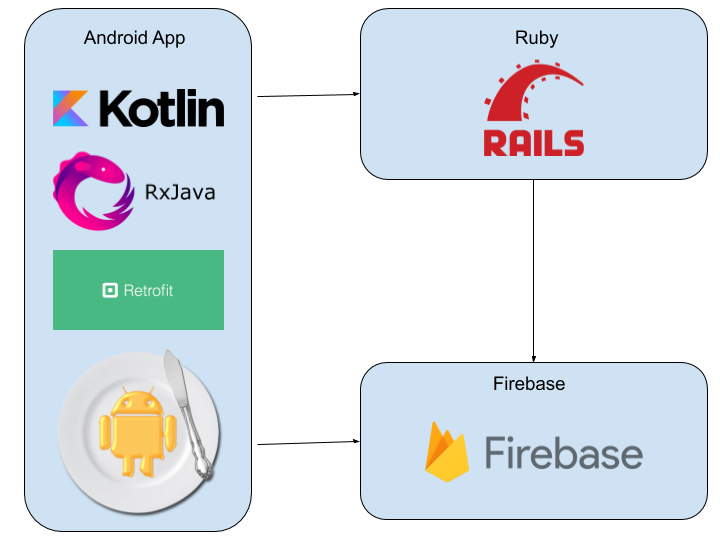
\includegraphics[width=0.7\textwidth]{SystemOverview.png}
  \caption[Overview of the Proposed System]{Overview of the Proposed System}
  \label{fig:systemoverview}
\end{figure}

As shown in Figure \ref{fig:systemoverview} the system consists of three parts, the Android mobile app, the Firebase backend and the Ruby backend.

The mobile app will communicate with both Firebase and the Ruby server as denoted by the arrows in the figure. The Ruby server will also have a communication to the Firebase backend in order to facilitate particular functionality such as notification scheduling as mentioned previously. 

It should be noted that the logos in Figure \ref{fig:systemoverview} represent the libraries used in each part of the system but this is not extensive, as some libraries simply do not have logos. A more complete list and their associated functionality is given in sections \ref{section:mobiletechused}, \ref{section:firebasetechused} and \ref{section:rubytechused}.

\subsection{Mobile App Technologies Used}
\label{section:mobiletechused}

\subsubsection{Language - Kotlin}
\label{arch:kotlin}

As outlined in section \ref{mobileapplicationsstateoftheart} Kotlin is now the language Google recommends for Android development. For this reason, and others outlined in section \ref{mobileapplicationsstateoftheart} Kotlin will be the language used for the Android app development aspect of this project rather than Java.

\subsubsection{Code Structure - Clean Architecture}
\label{section:cleanarch}

For the Android application aspect of this project the code will be using Clean Architecture, a code architecture developed by Robert Martin in his book "Clean Architecture: A Craftman's Guide to Software Structure and Design"\cite{cleanarchitecturebook}.

\begin{figure}[ht]
  \centering
      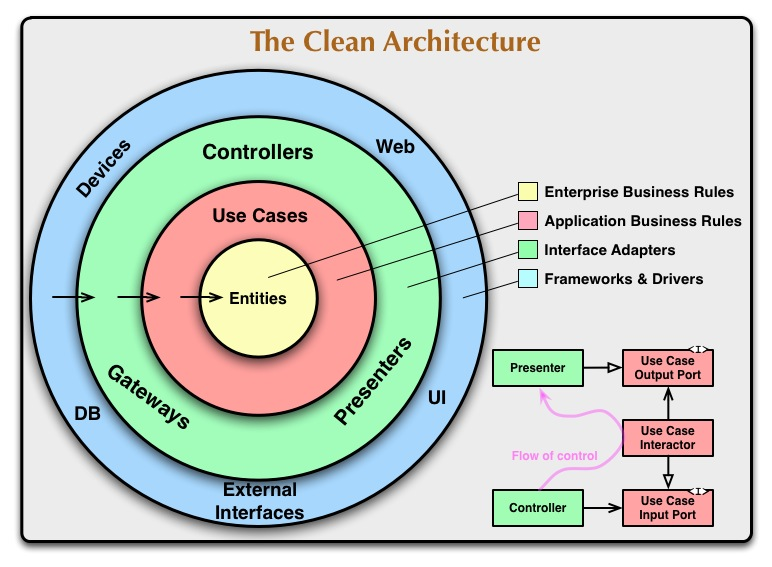
\includegraphics[width=0.7\textwidth]{cleanarchitecturemartinmodel.jpg}
  \caption[Clean Architecture Diagram]{Clean Architecture Diagram\cite{cleanarchitecturemartindiagram}}
  \label{fig:cleanarchitecturediagram}
\end{figure}

Figure \ref{fig:cleanarchitecturediagram} shows the approach to clean architecture as devised by Robert Martin. In this diagram the outer layers know about their immediate inner layer but holds no reference to any layer inside that. A layer also knows nothing of its outer layers.

This project will be using a slightly modified version of clean architecture which has been devised by the Android development team at the company Teamwork in order to handle some Android specific issues which this base version of clean architecture does not address.

\begin{figure}[ht]
  \centering
      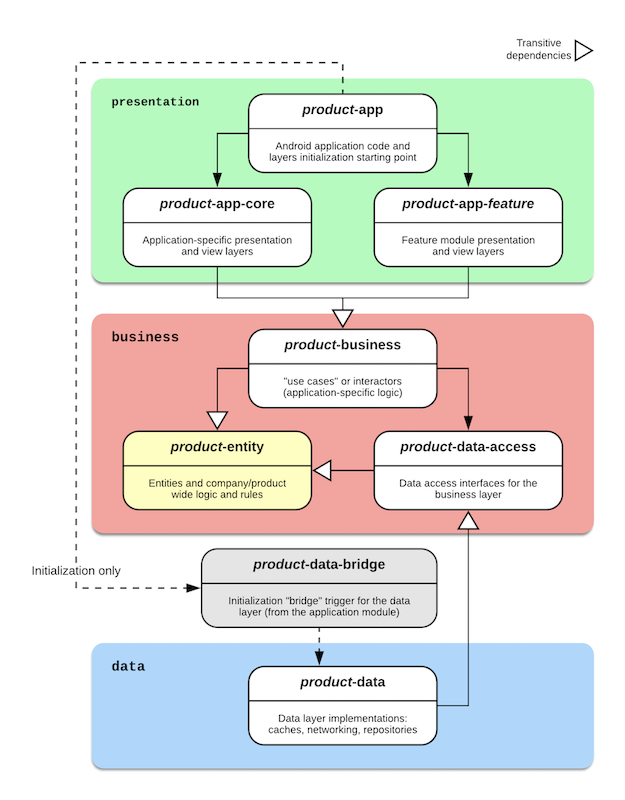
\includegraphics[width=0.7\textwidth]{clean_architecture_android_structure.png}
  \caption[Android Specific Clean Architecture Diagram]{Android Specific Clean Architecture Diagram\cite{teamworkcleanarchitecture}}
  \label{fig:teamworkcleanarchitecture}
\end{figure}

As seen in figure \ref{fig:teamworkcleanarchitecture} there are three distinct parts to this clean architecture setup, Data, Business and Presentation. In this implementation there are extra modules included to deal with Android specific problems in relation to clean architecture.

%The business-injection module is in place to allow the DI framework to successfully build a dependency graph in a multi-module project. 
The data-bridge modules exists only to initialise the DI graph for the data layer and contains no specific application logic.

The data layer covers operations related to network requests and database storage. In this project Firebase is used as the backend storage service and the Android libraries to access the Firebase API automatically handle caching. Therefore the data layer in this project will be used mainly for accessing Firebase but any extra work related to caching or threading will be unnecessary as the Firebase libraries handle these internally. The data layer will also be used to access the Ruby backend server but this will be in only limited circumstances given the relatively limited functionality of this server when compared to the Firebase backend.

The business layer is in charge of accessing the data layer functionality and applying any necessary application level business rules to the result obtained. This typically amounts to checking the validity of the data received and either just passing it on to the presentation layer when it is valid or passing some default value to the presentation layer when this data is not valid.

The presentation layer of this setup is in charge of calling the appropriate business layer methods when needed and obtaining a result. The presentation layer is also responsible for performing any transformations to the result obtained in order to make it suitable to show to the user.

While there are some clear cut differences between the presentation and business layers some functionality may seem like it could fall into either category. A common way of distinguishing responsibilities is to think of the presentation layer deciding the when and the business layer deciding the how. The presentation layer decides when something should be done, such as at the click of a button. The business layer decides how it should be done, for example whether it should happen asynchronously or not.

More in-depth detail on this exact clean architecture implementation can be found at \url{https://github.com/Teamwork/android-clean-architecture}. The only changes this project will make to this base setup is the conversion of any Java classes to Kotlin.

Clean Architecture will be employed extensively in this project as all classes in the mobile app will conform to  the layering and restrictions set on this layers by the Clean Architecture code structure.

\subsubsection{Dependency Injection - Dagger2}

This mobile app will use Dagger2 as the dependency injection framework of choice. While there are many DI frameworks available Dagger2 is maintained by Google and as seen in figure \ref{fig:androiddi} it is the only DI framework recommended for all sizes of Android app. 

\begin{figure}[ht]
  \centering
      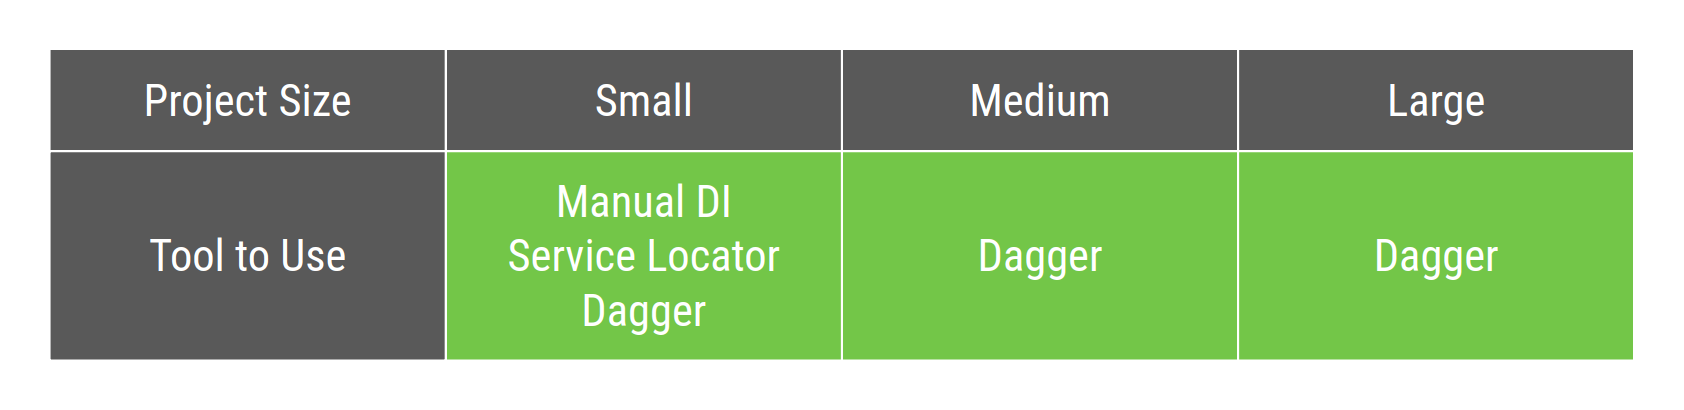
\includegraphics[width=0.7\textwidth]{androiddirecommendation.png}
  \caption[Android DI Framework Recommendations]{Android DI Framework Recommendations\cite{androiddi}}
  \label{fig:androiddi}
\end{figure}

The size of an Android app is based approximately on how many different screens it has. These approximate size definitions are outlined in figure \ref{fig:androidappsizes}.

\begin{figure}[ht]
  \centering
      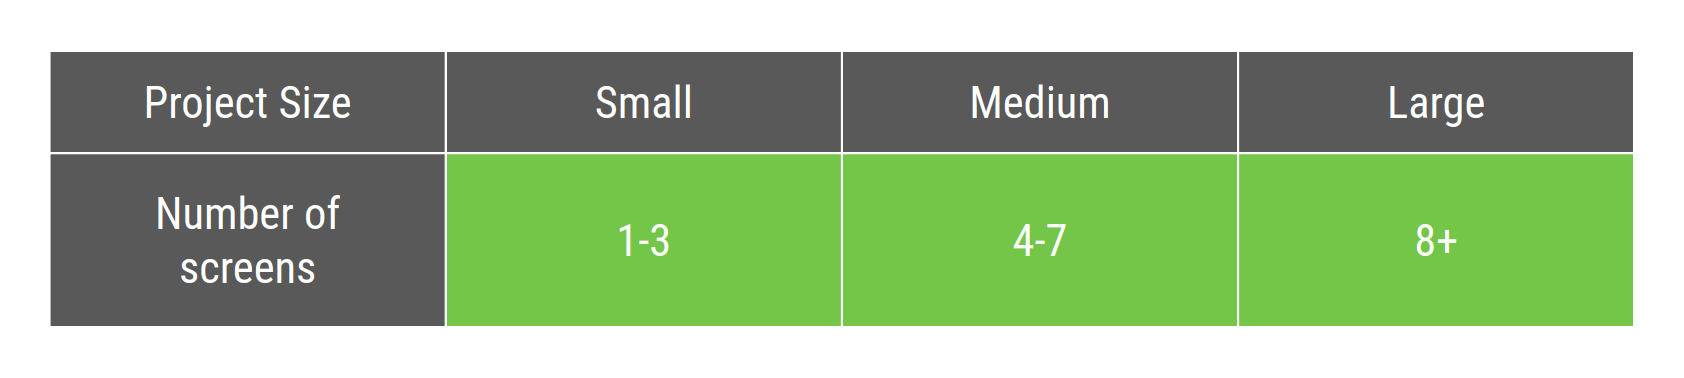
\includegraphics[width=0.7\textwidth]{appsizedef.png}
  \caption[Android App Size Approximations]{Android App Size Approximations\cite{androiddi}}
  \label{fig:androidappsizes}
\end{figure}

Dagger2 will be used extensively in this project as a means of keeping with the SOLID principles of Single Responsibility and Dependency Inversion. It is anticipated that almost all classes will use Dagger2 to inject dependencies.

\begin{figure}[ht]
  \centering
      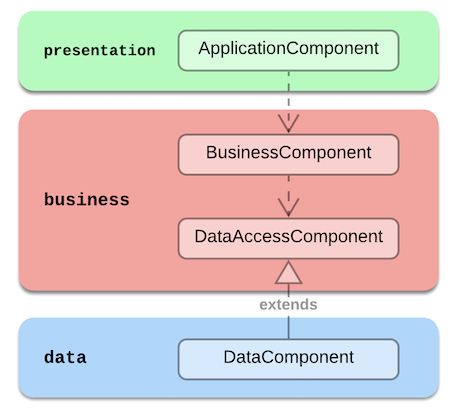
\includegraphics[width=0.7\textwidth]{clean_app_architecture_components.png}
  \caption[Dagger2 Component Graph Setup]{Dagger2 Component Graph Setup\cite{teamworkcleanarchitecture}}
  \label{fig:cleanarchitecturedicomponents}
\end{figure}

Shown in figure \ref{fig:cleanarchitecturedicomponents} is the setup for how Dagger2 will utilise multiple components in order to build a dependency graph across multiple modules

\subsubsection{AndroidX}

AndroidX refers to the Android support libraries which provide backwards compatibility to Android apps. It also encompasses Google's Android Jetpack suite of libraries.

AndroidX, despite officially being labelled as a group of support libraries, are a necessity in every Android project as many of the basic classes used in Android development come from it. There would therefore be far too much information to go into here if all AndroidX packages which are to be used were mentioned.

However, by leaving out the common uses of AndroidX which can be found in most, if not all, Android projects we can look at some of the more helpful features which come out of the Android Jetpack subset of libraries which will be used in this project.

\paragraph{Android KTX}

Android KTX acts as an add-on for the Kotlin language when used in Android. This library provides a set of extensions to Android classes which can replace verbose code with more concise versions which achieve the same functionality\cite{androidktx}.

\paragraph{Android Jetpack Navigation Component}

The Android Jetpack navigation component is a library which handles the boilerplate code associated with navigating between screens in an Android app.

While it makes up a minor part of mobile apps navigation in Android can often require a lot of boilerplate code to handle states. This code can often grow massive and lead it to be buggy and difficult to maintain.

The navigation component takes care of these problems as well as adding support for features which would normally be considered quite difficult to implement, such as deep linking.

In short the use of this library allows for a massive reduction in boilerplate code, handles difficult use cases and thus frees the developers time allowing them to focus on user facing features\cite{androidjetpacknavigation}.

There are many more helpful libraries available as part of the Android Jetpack suite. More information can be found on them at \url{https://developer.android.com/jetpack}.

The AndroidX libraries will be used heavily throughout this mobile app as they are now a standard in Android development and the exact uses are listed above.

\subsubsection{RxJava/RxAndroid}

RxJava is a library designed to allow for quick development of asynchronous and event-based programs using observable sequences\cite{rxjava}.

% This library uses an implementation of the Observer pattern to complete some background work then pass the result to a foreground thread.

By using RxJava and its RxAndroid extensions a lot of boilerplate code relating to threading can be avoided while also remaining conscious of the Android lifecycle with little effort on the part of the developer. 

% As RxJava is developed with asynchronous work in mind there is little for a developer to worry about in terms of race conditions or other common threading problems as these are handled by the library. 
\begin{figure}[ht]
  \centering
      
\includegraphics[width=0.7\textwidth]{rxjavabasicexample.png}
  \caption[RxJava Basic Observable Example]{RxJava Basic Observable Example\cite{rxjavamarblediagram}}
  \label{fig:rxjavamarblediagram}
\end{figure}

Figure \ref{fig:rxjavamarblediagram} shows one of the most basic examples of how RxJava emits items in an Observable. The arrow line indicates time passing. First the circle is emitted, then the pentagon, then the triangle and finally the thread terminates with an error. The thread can also continue on indefinitely or close without an error.

This is only one of the most basic examples with no other operations being performed on the items emitted. More detailed examples and diagrams can be found at \url{https://medium.com/@jshvarts/read-marble-diagrams-like-a-pro-3d72934d3ef5}.

The use of RxJava in this project will not be extensive as it is not anticipated for the use of separate threads to occur frequently. This is taking into account that Firebase, the main source of slow operations in this project, handles its own threads internally.

\subsubsection{Retrofit}

Retrofit is a library designed to turn a HTTP client into a Java interface. Retrofit essentially takes a remote REST API and by providing an interface which outlines the structure of the various request types the REST API uses, Retrofit handles generating the correct code for contacting the remote server with the query URL and all parameters formatted correctly\cite{retrofit}.

Retrofit will be playing a relatively small role in this project as it will only be used in interactions with the Ruby server which plays a limited role in this project.

Further information on Retrofit is used can be found at \url{https://square.github.io/retrofit/}.

\subsubsection{Butter Knife}

Butter Knife is a view binding library designed to reduce the boilerplate code associated with typical Android view binding by generating the necessary UI code at compile time\cite{butterknife}.

When a view exists but not in the same scope as the logic controller it is attached to, Android Studio will not recognise this mistake and allow a successful build despite the fact it won't work. By using Butter Knife an error is thrown at compile time which highlights this issue.

Butter Knife will be used quite extensively in this project as it will be in use in every screen presented to the user to bind all UI elements.

Further details on Butter Knife can be found at \url{https://jakewharton.github.io/butterknife/}.

\subsubsection{Glide}

Glide is an image loading and caching library for Android which handles all loading asynchronously. By using this library there is a massive reduction in boilerplate code and the developer can avoid working with difficult issues in regard to threading and background operations, as well as massively improving efficiency on the time-consuming and resource heavy task of image loading in Android.

Glide will not be used very much in this project as it is anticipated to be used mainly when loading images which are stored online, such as user profile pictures. All other images will be either packaged with the app or defined as vector images using XML.

Further details on the usage of Glide can be found at \url{https://github.com/bumptech/glide/blob/master/README.md}.

\subsubsection{Moshi}

Moshi is a library for converting JSON responses to POJO and vice versa.\cite{moshi}. It holds some significant improvements over similar libraries such as GSON in regards to speed and Kotlin support\cite{moshibettergson}.

Moshi will play a relatively small part in this project as it will be used only for interactions with the Ruby backend server and, as stated previously, this server will have a limited role in comparison to the Firebase backend.

\subsection{Firebase Technologies Used}
\label{section:firebasetechused}

\begin{figure}[ht]
  \centering
      
\includegraphics[width=0.7\textwidth]{Firebase_Logo.png}
  \caption[Firebase Logo]{Firebase Logo\cite{firebaselogo}}
  \label{fig:firebaselogo}
\end{figure}

While Firebase is technically a single technology provider, it encompasses many different types of features so it is still worth outlining here which of these will be used in this project.

\subsubsection{Firebase Authentication}

Firebase Authentication provides a drop-in UI solution for including a complete register and login flow in a mobile app. There are a lot of built in options such as allowing sign-in through Twitter, Google and other sites but for this project the default email and password sign-in will be used.

A detailed overview of Firebase Authentication can be found at \url{https://firebase.google.com/docs/auth}.

Firebase Authentication will form the one and only register and login procedure for users in this project. The Firebase UI for registering or logging in will be the first screen presented to the user on startup of the app. Once signed in, it is expected that this screen will rarely, if ever, be used again by the user. As with most services requiring authentication it is expected that once signed in a user will not sign out again for the sake of convenience.

\subsubsection{Firebase Cloud Firestore}

Firebase Cloud Firestore is a realtime NoSQL cloud based storage solution which allows for many clients to quickly access up-to-date information.

\begin{figure}[ht]
  \centering
      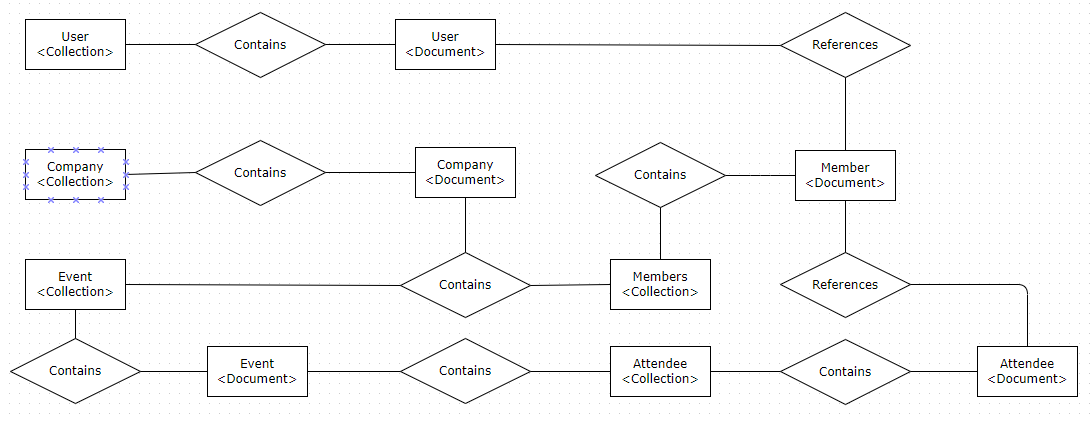
\includegraphics[width=0.7\textwidth]{DBDesign.PNG}
  \caption[Proposed Database Design]{Proposed Database Design}
  \label{fig:databasedesign}
\end{figure}

In Figure \ref{fig:databasedesign} is the proposed design of the Firestore NoSQL database. 

The structure of the Firestore database is a document-based NoSQL database, each document is made up of key-value pairs for the data and subcollections which contain further collections of documents. 

In this diagram we can see collections contain documents and documents, in turn, may contain collections. Unfortunately, due to the lack of a strictly enforced data structure as with SQL databases, many modelling tools for NoSQL databases do not seem to contain the tools for detailing key-value pairs of data.

The two main collections making up this database will be 'User' and 'Company'. These then contain documents of an individual User or Company in turn. While the User collection remains simplistic, the Company collection is more complicated due to the data points associated with a company in this project. 

Each Company document will contain the subcollections of 'Event' and 'Members'. Each Member document will reference an already existing User document. Each Event document will contain a further subcollection of 'Attendees' with each Attendee document referencing a company member.

Aside from any subcollections each document will also contain any other required information for its data. For example an Event document will contain event name, location and so forth on top of its Attendees subcollection. 

The exact features of Firestore are far too extensive to list here but details can be viewed at \url{https://firebase.google.com/docs/database/rtdb-vs-firestore}.

Firestore will be used extensively in almost every facet of this project as it will need to be accessed by the mobile app for every display of information as well as by the Ruby server to allow for the required database access.

\subsubsection{Firebase Cloud Messaging}

FCM is a component of Firebase which allows for sending messages reliably to connected client devices. In the case of mobile devices, these are almost always then shown as notifications.

Further details on FCM can be found at \url{https://firebase.google.com/docs/cloud-messaging}.

FCM will be used for all instances of notification delivery in this project.

\subsection{Ruby Server Technologies Used}
\label{section:rubytechused}

\subsubsection{Ruby on Rails}

\begin{figure}[ht]
  \centering
      
\includegraphics[width=0.7\textwidth]{railslogo2.png}
  \caption[Ruby on Rails Logo]{Ruby on Rails Logo\cite{rubyonrailslogo}}
  \label{fig:rubyonrailslogo}
\end{figure}

Ruby on Rails is a library for the Ruby language which provides an easy to setup environment and quick development of applications\cite{rubyonrails}.

As this project will be using the Ruby server in a limited number of cases and purely as an API, Ruby on Rails is chosen as it provides built-in tools for creating exactly this kind of setup quickly\cite{rubyonrailsapi}.

Rails applications also come with a default database using SQLite. In this project the data storage will be handled primarily by Firebase, however as the ruby server is required to generate a human readable ID for each new company created, this SQLite database will be used as a convenient way to auto-generate an ID for new companies. This will then be stored by Firebase with all other data\cite{rubydatabase}.

Rails also gives the benefit of strictly enforcing an MVC code architecture which in turn tends to produce more robust code\cite{rubycodestructure}.

Further details on Ruby on Rails can be found at \url{https://rubyonrails.org/}. Details on specifically the API features of Rails can be found at \url{https://guides.rubyonrails.org/api_app.html}.

Rails will form the entirety of the Ruby server in this project.

\subsection{How These Technologies Are Used}

The proposed use of the outlined technologies and the interactions between different parts of the system are as follows:

The mobile app code structure will be using Clean Architecture as detailed in section \ref{section:cleanarch}. In an effort to make code as reusable as possible and to increase adherence to the SOLID principles of Single Responsibility and Dependency Inversion, Dagger2 will be used to provide instances of all possible classes throughout the project.

The mobile app will need to have means of communication with both Firebase and the Ruby server. Firebase includes all networking and threading operations as part of its libraries but connection with the Ruby server will need to be handled by the developer. In this scenario RxJava, Retrofit and Moshi are all used. Retrofit is the means of connecting to the server and receiving a response, Moshi will parse that response into usable objects in code and RxJava will handle the threading operations which come with networking functionality.

As listed in section \ref{section:mobiletechused} other libraries such as Glide and the AndroidX suite will be used. The AndroidX libraries will be used extensively for various pieces of functionality throughout the app. Glide will be used in far more limited cases. In order to avoid too much repetition here on what functionality these libraries offer details can be found above in section \ref{section:mobiletechused} giving an overview of their benefits.

The Firebase backend will provide most of the server side functionality for this project, most heavily used will be Firebase Cloud Firestore for storing user data.

The separate Firebase components listed in section \ref{section:firebasetechused} will not actually have any direct interaction with one another in this project.

Most interactions with the Firebase backend will come from the mobile app through the use of the various Firebase libraries. Firebase Cloud Storage will be in charge of providing the data on events, people and companies. Firebase authentication will provide the means of new users registering and logging into the mobile app and FCM will provide the mechanism for sending notifications to users at the appropriate times, such as for event invitations, reminders and so forth.

Finally the Ruby server will provide some limited functionality which Firebase does not support currently. Within the scope of this part of the system is creating a new company ID and scheduling when notifications are to be sent.

The Ruby server is in charge of creating a new company ID as it provides a convenient way of generating unique human readable IDs for each company whereas Firebase Cloud Storage does not. By default Ruby on Rails comes will an SQLite database. This database will not be used for data storage but by creating a new entry for each new company the auto-generated ID created by the database gives a simple unique value which can then be passed onto Firebase.

Firebase does not currently support sending a notification at a specific time but by including the Ruby server in the notification process a workaround can be found. When some action is taken which results in notifications being sent sometime in the future the Ruby server can schedule when to connect to Firebase and send the notification.

For these purposes there will also e a direct means of interaction between the Ruby server and the Firebase backend.

\section{Risk Assessment}
\label{section:risks}
% Identify any potential risk precluding you from successfully complete your project. This section is really important and often neglected by students resulting in fatal risks occurring in some projects. Make sure to give this section the time it requires. Classify the risk according to their importance, possibility of arising and enumerate the decisions you can make to anticipate them or mitigate them (in case they finally arise). Table \ref{tab:ProjRisks} may help with this classification. This section should include your mitigation approach for any critical risks.

% \begin{table}[h]
% \centering
% \scriptsize
% \caption{Initial risk matrix}
% \begin{tabular}{|p{2cm}|p{2cm}|p{2cm}| p{2cm} |p{2cm}| p{2cm}|}
% \hline \bf Frequency/ Consequence & \bf 1-Rare & \bf 2-Remote & \bf 3-Occasional & \bf 4-Probable & \bf 5-Frequent\\ [10pt]

% \hline \bf 4-Fatal & \cellcolor{yellow!50} & \cellcolor{red!50} & \cellcolor{red!50} & \cellcolor{red!50} &\cellcolor{red!50} \\ [10pt]

% \hline \bf 3-Critical &\cellcolor{green!50} & \cellcolor{yellow!50} & \cellcolor{yellow!50} & \cellcolor{red!50} &\cellcolor{red!50} \\ [10pt]

% \hline \bf 2-Major & \cellcolor{green!50} & \cellcolor{green!50} & \cellcolor{yellow!50} &\cellcolor{yellow!50} &\cellcolor{red!50} \\ [10pt]

% \hline \bf 1-Minor & \cellcolor{green!50} & \cellcolor{green!50} & \cellcolor{green!50} &\cellcolor{yellow!50} &\cellcolor{yellow!50} \\ [10pt]
% \hline
% \end{tabular} \\
% \label{tab:ProjRisks}
% \end{table}

\subsection{Risk No. 1}

\textbf{Description}

Firebase backend goes down.

\textbf{Consequences}

Newly entered information from Firestore will not be made available to users.

\textbf{Severity}

Critical

\textbf{Possibility of Occurring}

Rare

\textbf{Risk Mitigations}

Unfortunately not much can be done in the event that Firestore somehow becomes unresponsive as this is the backbone of the app. However as Firebase is owned and backed by Google the odds of the service becoming unresponsive are incredibly rare. 

Besides this the Firestore library for Android comes with caching functionality built in. In such an event users will still be able to view the latest cached information on their device, also any newly entered data will be cached until such time as it can be persisted to the cloud based backend.

\subsection{Risk No. 2}

\textbf{Description}

Unable to complete sprints due to time constraints

\textbf{Consequences}

In such a case the app will be missing planned features and bugs may not be fixed.

\textbf{Severity}

Major

\textbf{Probability of Occurring}

Probable

\textbf{Risk Mitigations}

The chances of this occurring in the development of the Ruby backend or the Firebase setup is very unlikely given the limited functionality and ease of setup of these two parts of this project. This risk is therefore almost entirely a risk for the mobile app development.

The only mitigation in this scenario is to consistently follow the sprint outline devised in section \ref{section:implementationplan} and, when possible, get to work on the next sprint early.

By doing this and strictly following the concept of the MVP of this app, the project development phase can still end with an app which provides a high degree of value despite missing some planned features/functionality.

\subsection{Risk No. 3}

\textbf{Description}

Functionality differences between Android OS versions

\textbf{Consequences}

Users on different Android OS versions, particularly older versions, may experience non-typical or unexpected behaviour when using the app.

\textbf{Severity}

Minor

\textbf{Possibility of Occurring}

Probable

\textbf{Risk Mitigations}

While this is an issue known to occur in Android apps it is incredibly rare that this will affect the actual logic of the app. What is far more common is that UI elements are affected by this issue in that styling may not be applied correctly and thus UI elements which employ certain known troublesome classes can appear differently depending on the OS version.

While this risk is probable in its likelihood to happen, the chances of it adversely affecting  a user and preventing them from using the app is practically non-existent. 

These issues most commonly occur on devices running Android OS version 22 or lower. Therefore to mitigate this issue, and to allow reduction in handling various edge cases which come with older Android versions, this project will set Android version 23 as the minimum OS version the app can be used on.

Furthermore there are also well known workarounds for these styling issues which should be employed consistently over the standard classes provided for styling which in turn will yield consistent results across devices.

\section{Methodology}
\label{section:methodology}
% Describe your personal approach on how to tackle the different parts of this project, including:
% \begin{itemize}
%     \item How to tackle the needed research to fulfill the background chapter. 
%     \item How to set up your Computer Science skills to the project needs (e.g., describe your plan to learn any new technology involved on the project that you are not familiar with). 
%     \item What core project managing approach will you follow (e.g., Waterfall, Scrum, etc).
% \end{itemize}

\subsection{Learning New Technologies}

In regard to learning new technologies I am already somewhat well experienced in working with Android including each of the libraries listed in section \ref{section:mobiletechused}. I have also used each of the Firebase features listed in section \ref{section:firebasetechused} quite extensively in the past.

The main part of this project implementation requiring practice and research is the use of Ruby on Rails for the server backend. Due to the relatively limited scope of the Ruby server and the expected time constraints by the time the implementation phase of this project comes about, the plan for learning how to use this technology will focus only on learning what is absolutely needed rather than obtaining a broad knowledge. 

I have already taken steps in reviewing how to setup a Ruby on Rails server which acts only as an API interface. 

From this initial learning I believe the Ruby aspect of this project will be relatively short as Rails provides a quick setup tool for this exact use case. Further to this the Firebase documentation provides various examples of using Firebase in Ruby. Given these factors the Ruby part of this project is expected to be short and, relative to everything else, quite simple.

\subsection{Project Management Approach}

The development approach to be taken in this project will be Scrum with a sprint time of 2 weeks.

\section{Implementation Plan Schedule}
\label{section:implementationplan}
% Come up with a schedule for the remaining time (including second semester), so as to describe how do you envision to achieve the implementation of your project by the end of semester 2. This plan SHOULD be ambitious but MUST be realistic and SHOULD be informed by early prototyping and MUST be discussed with your term 1 supervisor.

\begin{longtable}{ |p{4cm}|p{10cm}|  }
		\hline
		\hline
		\textbf{Starting Date} & \textbf{Working On} \\
		\hline
		January 6th & 
		\begin{itemize}
		    \item Setup FirebaseAuth
		    \item Setup Firebase Cloud Storage
		    \item Setup FCM
		    \item Setup clean architecture mobile project structure
		    \item Setup Ruby on Rails for Ruby backend
		\end{itemize}\\
		\hline
		January 20th & 
		\begin{itemize}
		    \item Add FirebaseAuth to mobile app to allow for sign up/sign in
		    \item Create Ruby API for adding a new company
		    \item Add new company to Firebase Cloud Storage from Ruby server
		    \item Create mobile frontend for adding a new company
		    \item Create mobile frontend for users to join a new company
		    \item Create mobile frontend for users to view the events they are invited to
		\end{itemize}\\
		\hline
		February 3rd & 
		\begin{itemize}
		    \item Create mobile frontend for an admin to create a new event
		    \item An admin can set event-specific user details
		    \item Allow users to view the list of members of their company
		\end{itemize}\\
		\hline
		February 17th & 
		\begin{itemize}
		    \item Allow users to respond to an event invite
		    \item A user will receive a notification when invited to an event
		    \item A user can respond to event invites directly from the notification
		    \item A user will receive a notification for an upcoming event
		\end{itemize}\\
		\hline
		March 2nd & 
		\begin{itemize}
		    \item Update event details screen to show event location on a map
		    \item Implement app rating to allow users to give feedback on ease of use and reduction in difficulties experienced
		    \item Add mobile frontend to allow a user to view their own profile
		    \item Allow a user to view another user's profile
		\end{itemize}\\
		\hline
		March 16th &
		\begin{itemize}
		    \item Create mobile frontend for admins to view membership requests
		    \item Update join company functionality to now make a request rather than immediately join
		    \item Allow a user can edit their own profile
		\end{itemize}\\
		\hline
		April 6th &
		\begin{itemize}
		    \item An admin can set times for event reminders
		    \item An admin can make another user an admin
		\end{itemize}\\
		\hline
    \caption{Sprint Schedule}
	\label{table:sprints}
\end{longtable}

The remainder of the project implementation phase will be dedicated to working on any bug fixes or improvements which should be made to the system. The remaining time is also partially set aside for working on the implementation report.

\section{Evaluation}
\label{section:evaluation}
% Come up with an evaluation plan that allows you to measure how much have you actually achieved the goals of your project. This again is a section that is often neglected where students loose marks. How do you plan to measure the output of your project? A binary it works/does not work is insufficient. You need to be able to quantify the success against both the functional requirements and the initial idea. These are not the same as you may meet all function requirements outlined but not solve the overall problem because you have failed to revisit these and update them with new information which you learn as you are developing the project.

As shown in section \ref{section:implementationplan}, in the sprint beginning February 17th, one of the goals for this sprint is to implement user feedback.

This will be the way in which users can give a rating on the app, the usual 1 - 5 stars, as well as include any comments they have to give. As this app is the only user facing portion of the project any issues which occur due to problems in the Ruby or Firebase backends will also be reflected in this rating.

The top apps on the Google Play Store tend to have a rating of roughly 4 stars\cite{appstorerating}. Quite often 4 stars tends to be the minimum rating which apps aim to achieve therefore the same idea will be applied here. by taking the in-app star rating as a percentage, a score of 80\% or more will be taken to mean the project has been successful in achieving its goals.

Despite referencing Google Play Store ratings here the proposed user feedback will be separate. It will follow a very similar concept but by making this an in-app rating, customisations can be made on the type of feedback given. Feedback can be requested on very specific metrics, such as ease of event creation, reduction in organisation difficulties compared to previously used event management systems and so forth. This kind of feedback would prove far more useful than the generic good or bad review which is typically left on the Play Store. This feedback can then also be aggregated in Firebase to more easily allow for any desired data analysis.

\section{Prototype}
\label{section:prototype}
% Although you do not have a fully functional project yet, you should show wireframes, snapshots or representation on how do you envision your project to look once the implementation phase has been completed. The nature of this section will vary significantly from project to project and can include anything from code snippets to snapshots of service deployments. Any prototyping you have done during the term should be summarized here that has not been captured in earlier sections. For example if you are planning to host your project using AWS in an EC2 instance you should have at least created a "hello world" setup to determine the basics, this probably should have been discussed in section \ref{sec:Arch}.

This section gives a general idea on the look and functionality of the finished project. A prototype for the Firebase implementation is not included in this section as Firebase is a third party backend implementation which requires a client to work. Therefore the results of data stored by Firebase or notifications sent are shown as part of the mobile app prototype. 

All features in the mobile app prototype are shown but some of these will be unavailable if the user is not an admin. These will be highlighted in section \ref{section:mobileappprototype} when appropriate.

\subsection{Mobile App Prototype}
\label{section:mobileappprototype}

\begin{figure}[ht]
  \centering
      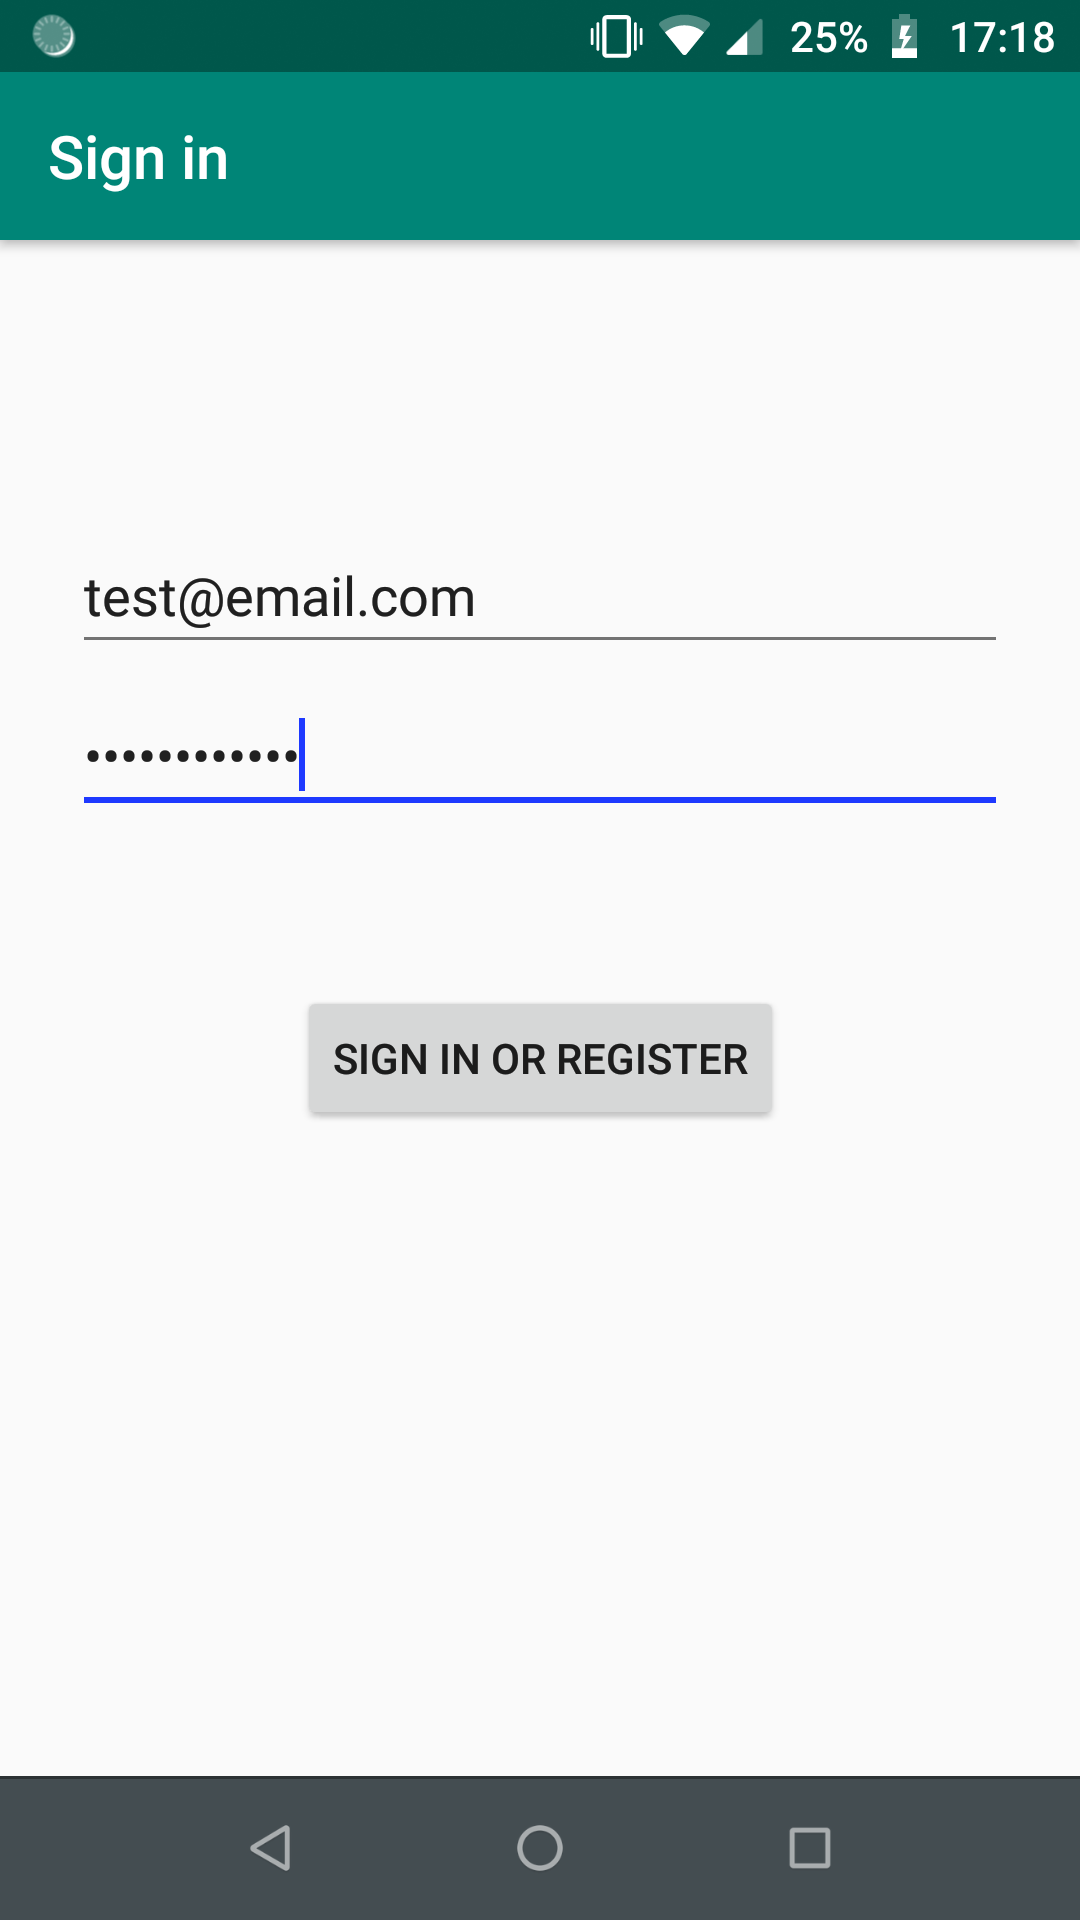
\includegraphics[width=0.7\textwidth]{SignInRegister.png}
  \caption[Mobile App Prototype Sign In/Register Screen]{Mobile App Prototype Sign In/Register Screen}
  \label{fig:signInRegister}
\end{figure}

Shown in Figure \ref{fig:signInRegister} is the outline of the Sign In/ Register screen for users to create an account for themselves or sign into an existing account. In the final project this screen will be handled by Firebase Authentication which provides a built-in sign in and register UI.

\clearpage
\begin{figure}[ht]
  \centering
      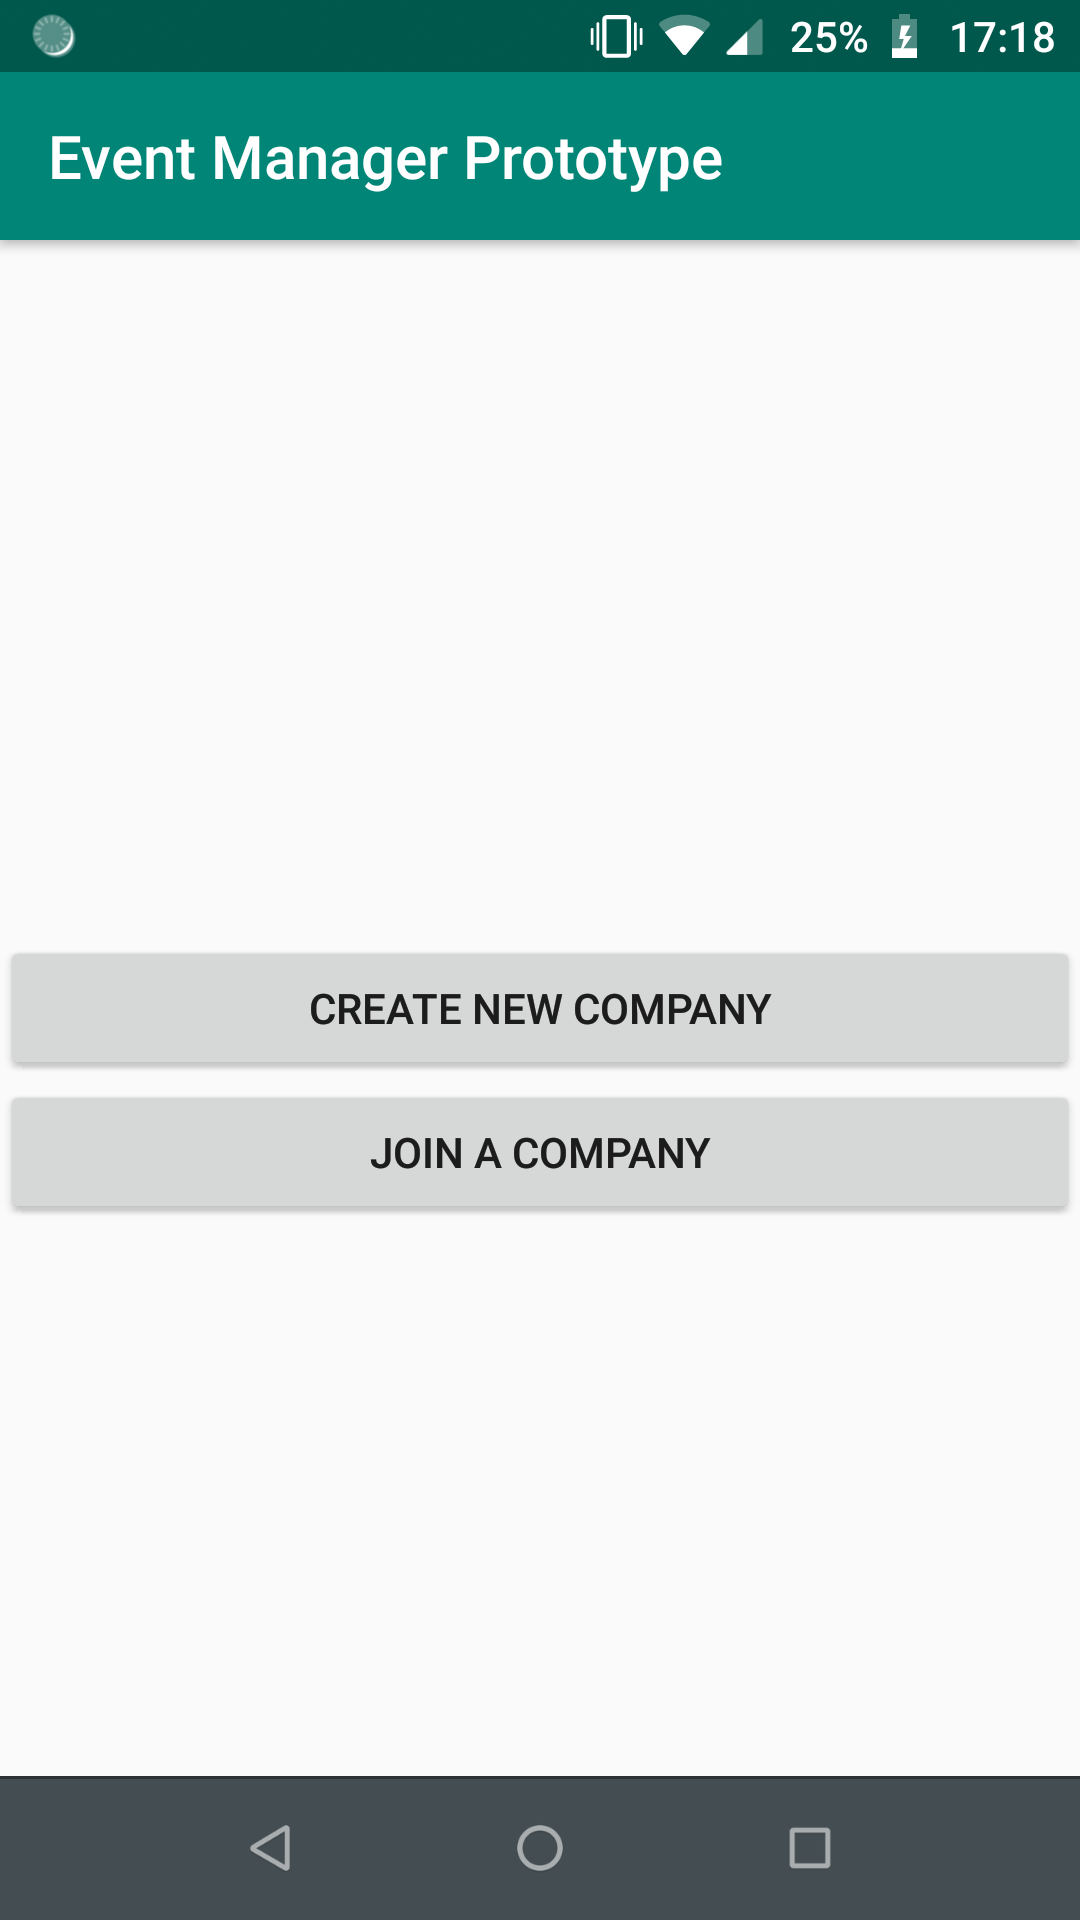
\includegraphics[width=0.7\textwidth]{CreateJoinCompany.png}
  \caption[Mobile App Prototype Create/Join Company Screen]{Mobile App Prototype Create/Join Company Screen}
  \label{fig:CreateJoinCompany}
\end{figure}

Once a user has created their account they will be presented with the screen shown in Figure \ref{fig:CreateJoinCompany}. Here they will be presented with the option of either creating a new company or joining an already existing company.

\clearpage
\begin{figure}
\centering     %%% not \center
\subfigure[Create Company Screen]{\label{fig:a}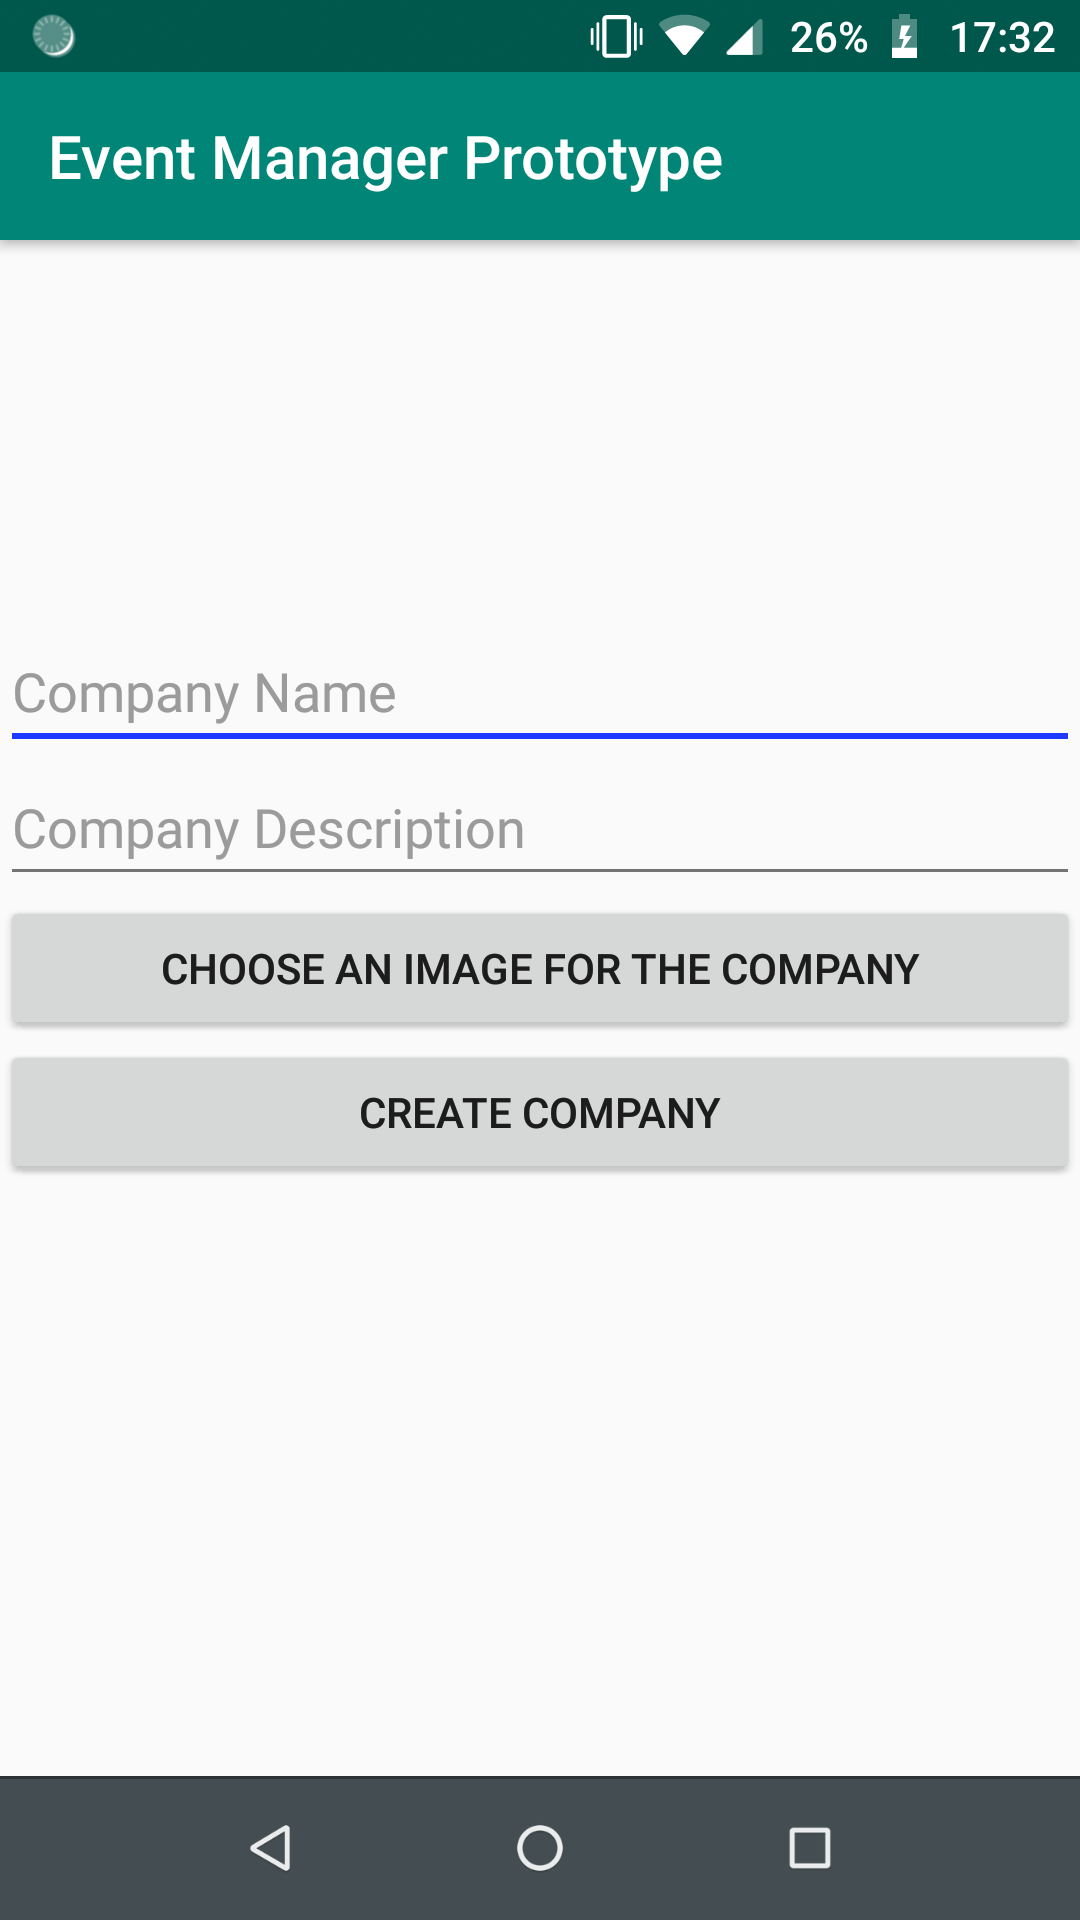
\includegraphics[width=0.48\textwidth]{CreateCompany.png}}
\subfigure[Join Company Screen]{\label{fig:b}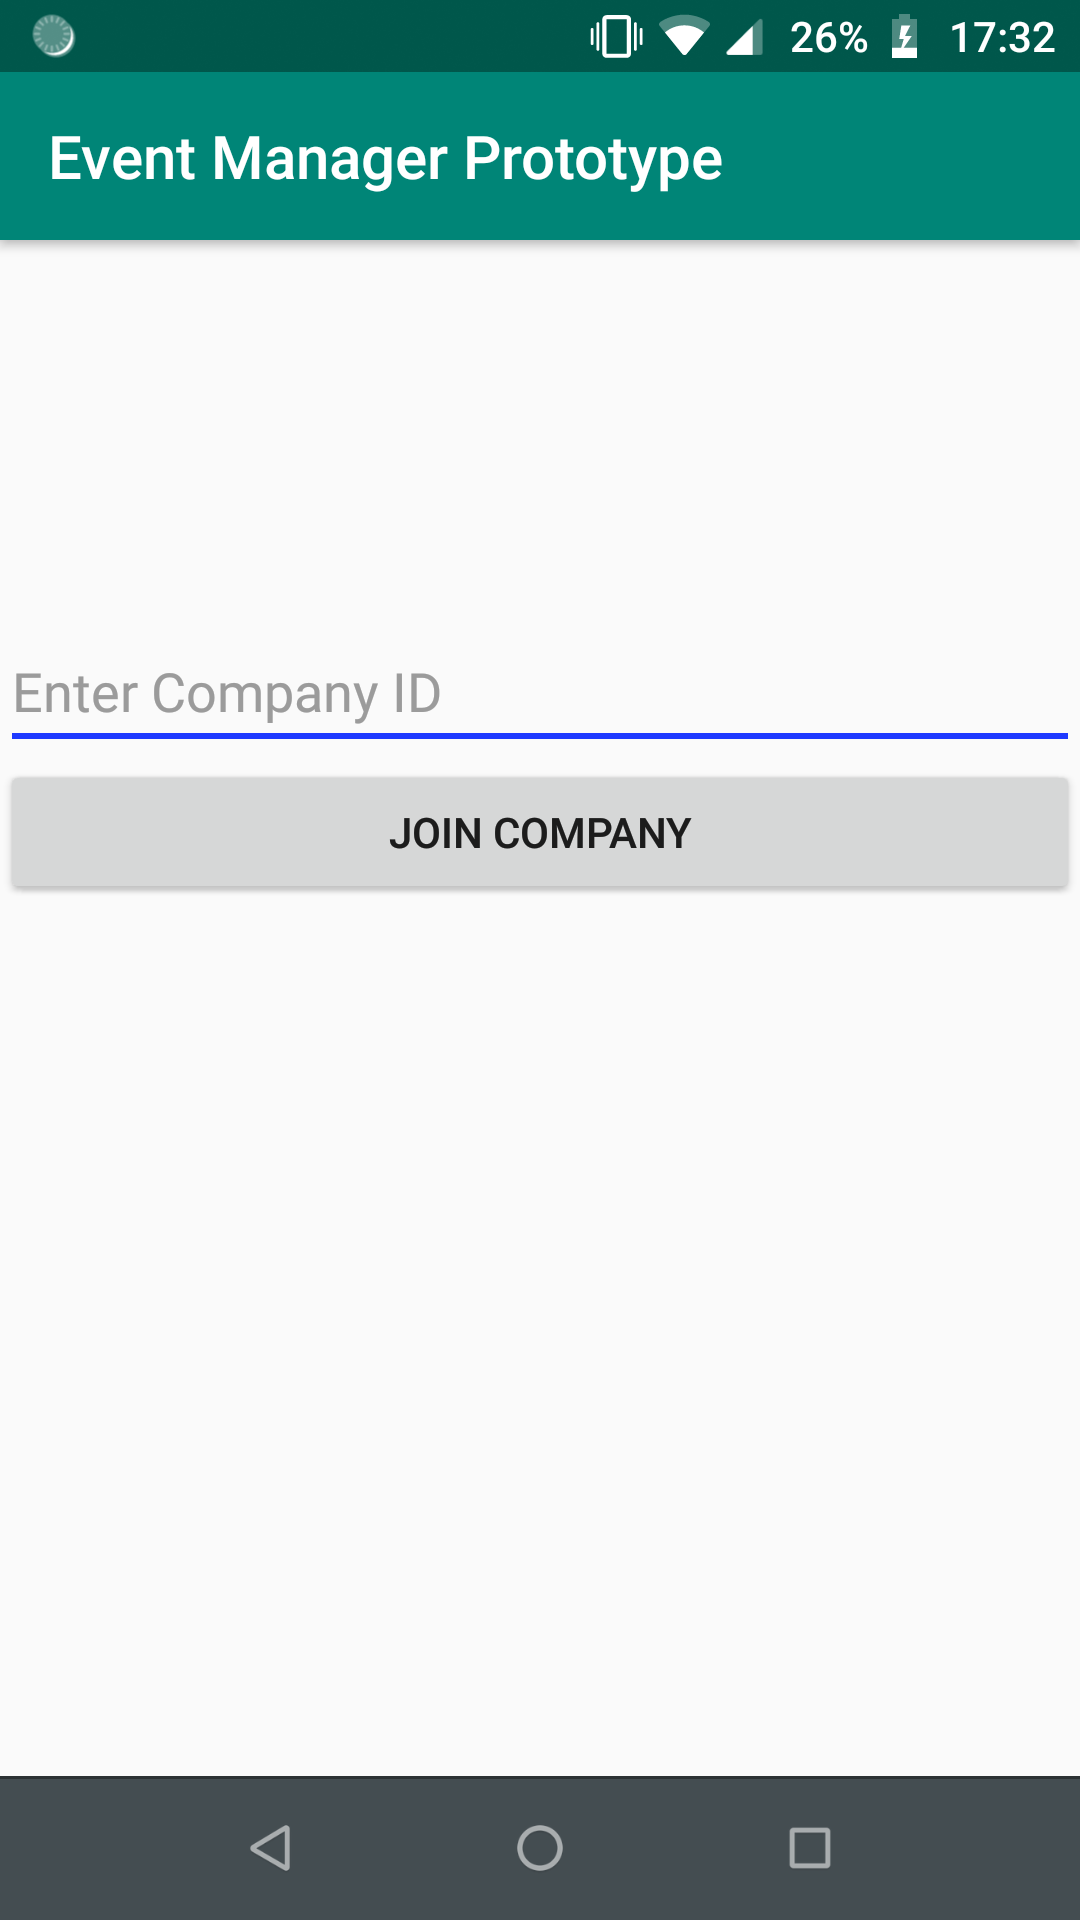
\includegraphics[width=0.48\textwidth]{JoinCompany.png}}
\caption{Mobile App Prototype Create and Join Company Screens}
\label{fig:CreateAndJoinCompanyScreens}
\end{figure}

Following on from the options presented in Figure \ref{fig:CreateJoinCompany}, in Figure \ref{fig:CreateAndJoinCompanyScreens} is shown the new options presented depending whether a user has chosen to create a new company or join an existing one. 

For creating a company the user can enter the company name, a description of the company and choose a company image. When joining a company a user must simply enter the company ID to make a membership request.

\clearpage
\begin{figure}[ht]
  \centering
      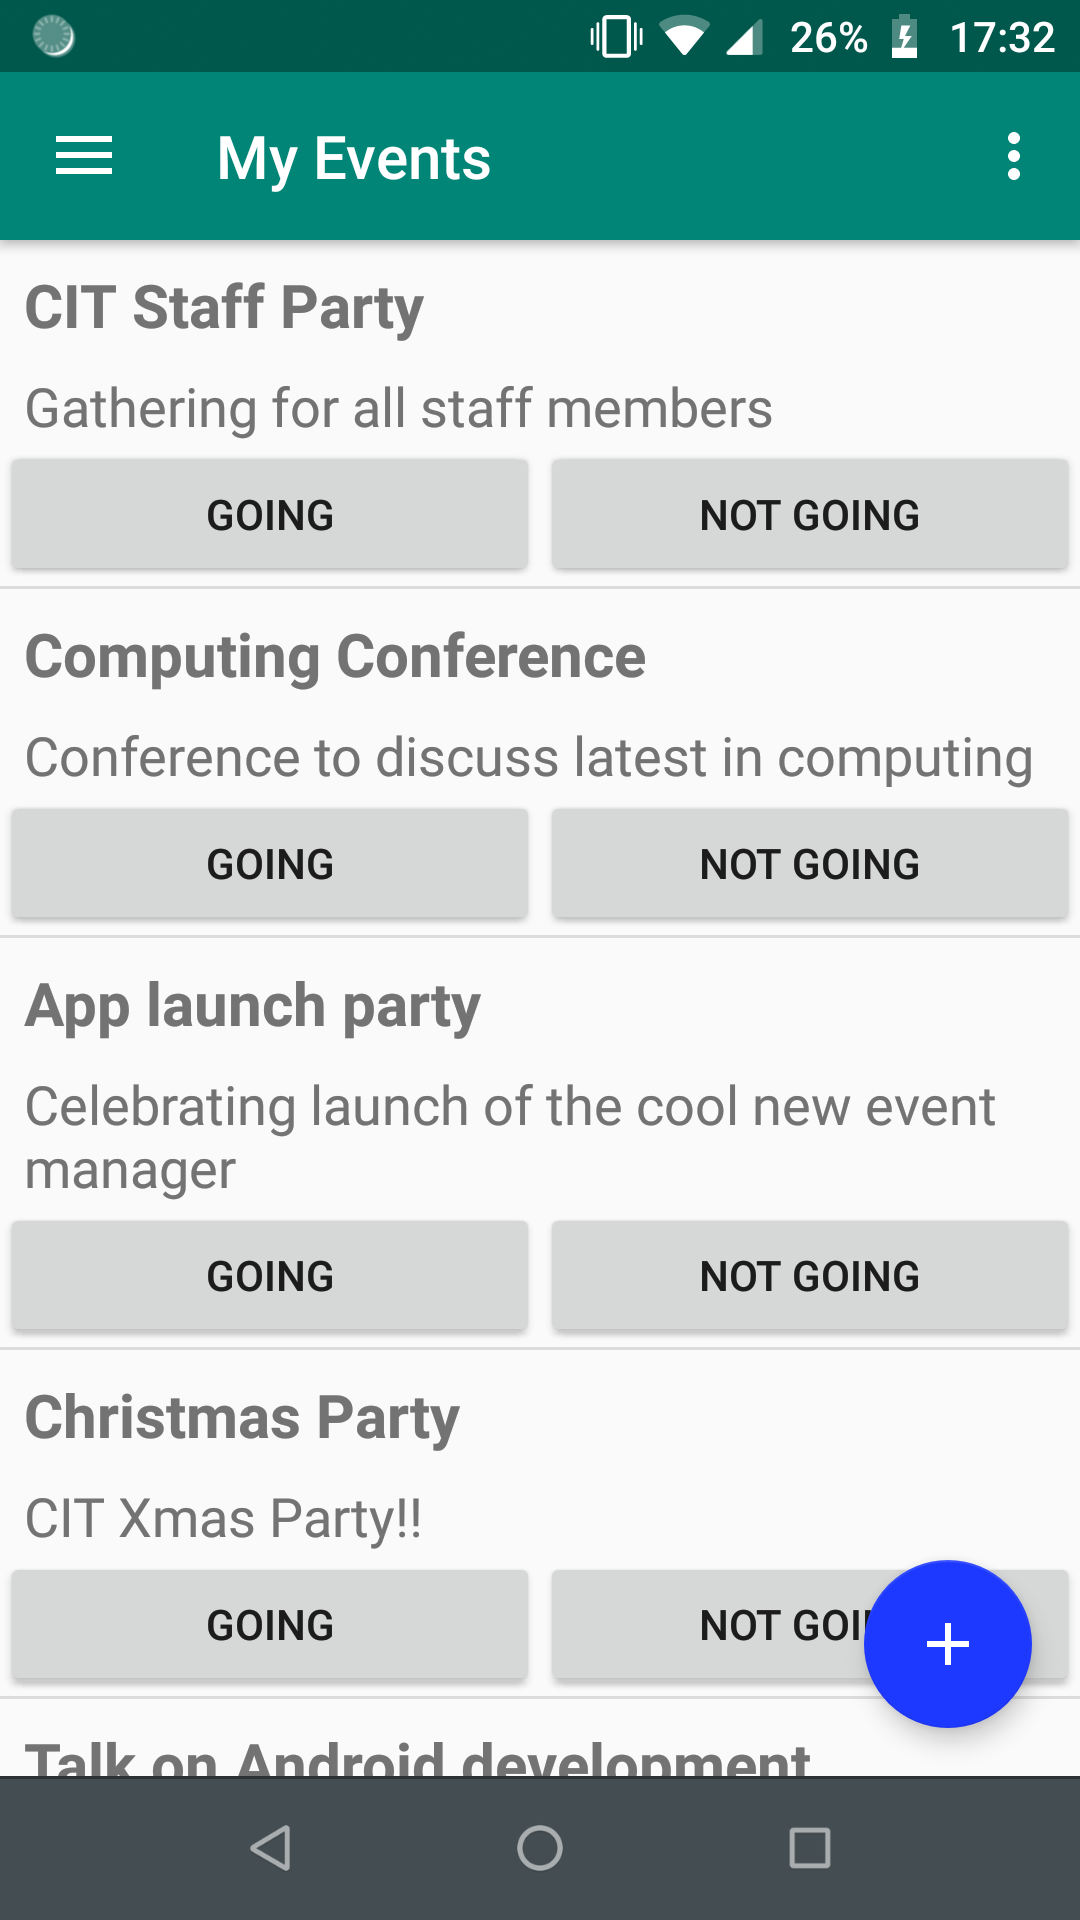
\includegraphics[width=0.7\textwidth]{EventList.png}
  \caption[Mobile App Prototype Event List]{Mobile App Prototype Event List}
  \label{fig:EventList}
\end{figure}

After completing the sign in and company creation process a user is able to gain full access to the app's features. First to be shown is the list of events as shown in Figure \ref{fig:EventList}. This screen shows the list of events the user is invited to and provides options for responding to those invites.

Also provided in this screen is a means of creating a new event through the blue '+' button in the lower right hand corner. This is a feature available to admins only. For users who are not admins this button will not be shown.

\begin{figure}[ht]
  \centering
      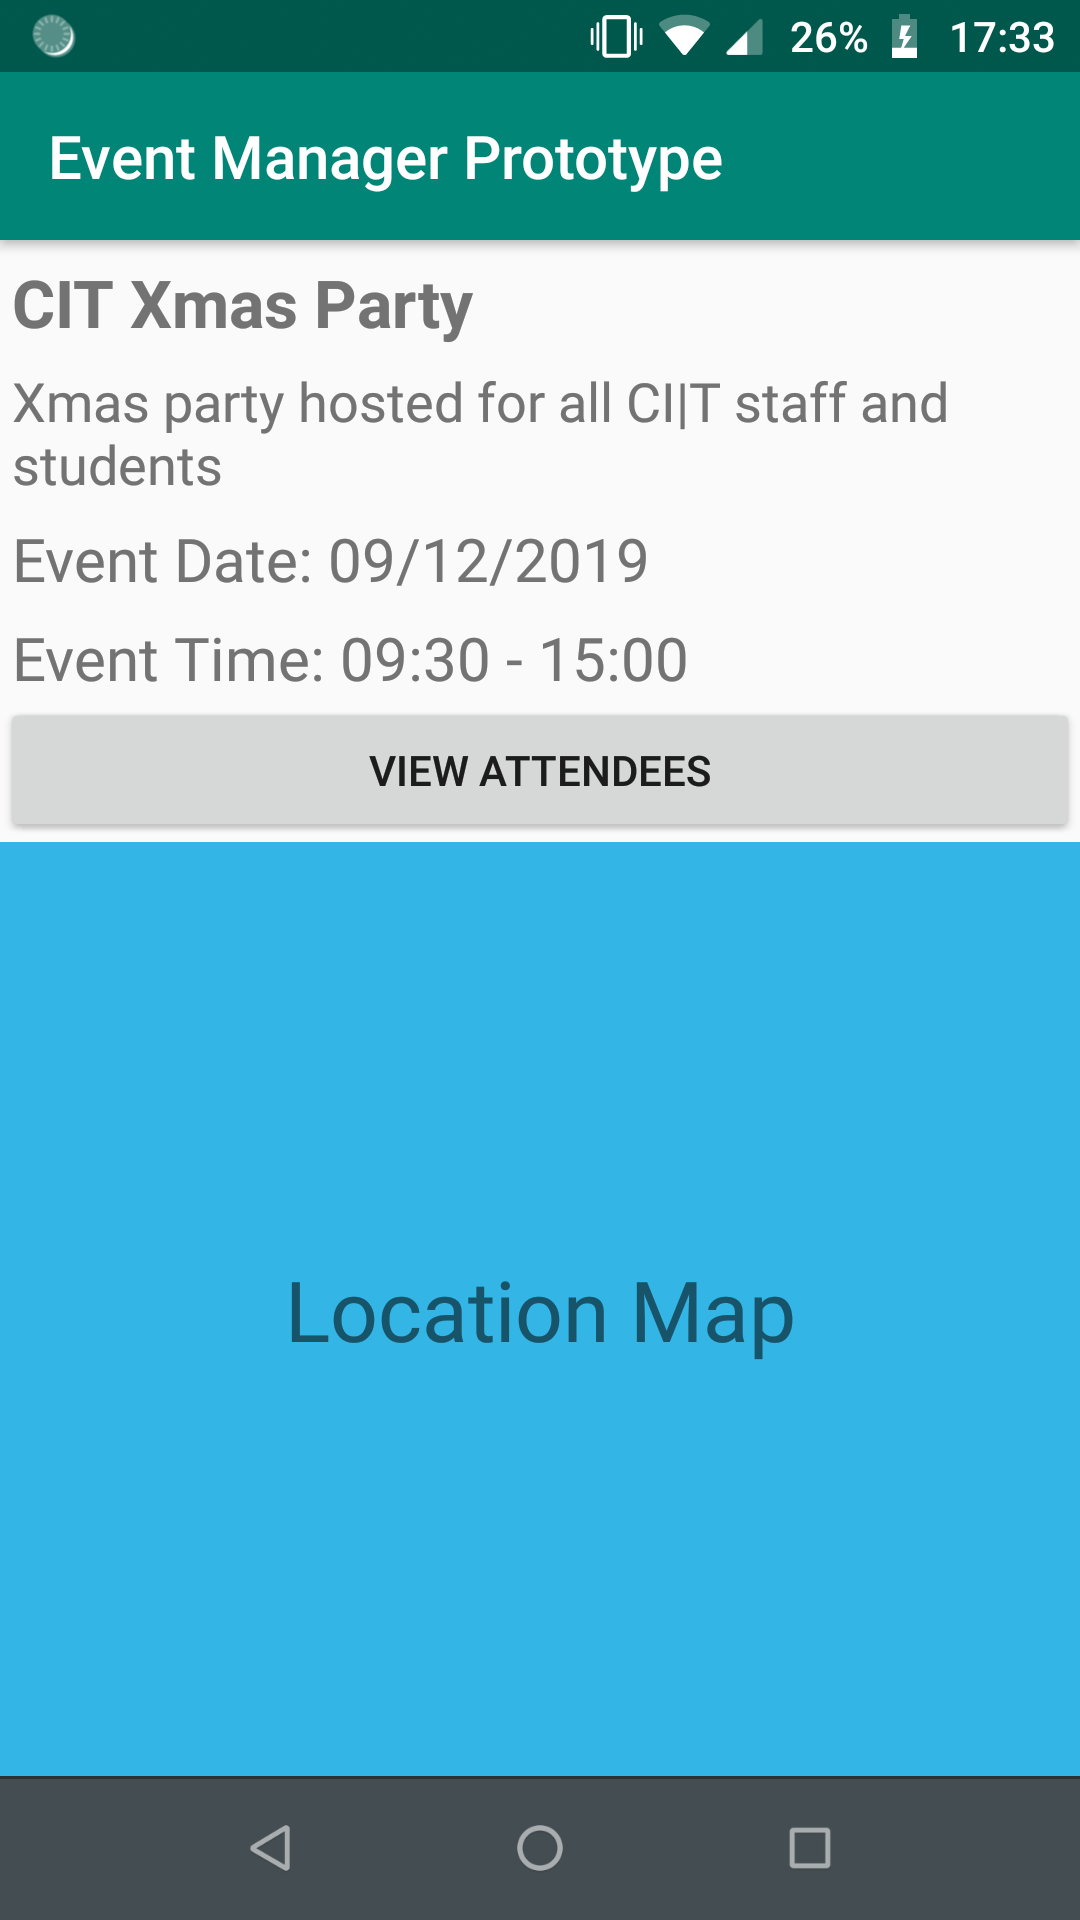
\includegraphics[width=0.7\textwidth]{EventDetail.png}
  \caption[Mobile App Prototype Event Details]{Mobile App Prototype Event Details}
  \label{fig:EventDetail}
\end{figure}

When the user clicks on an event from the events list they will then be provided with further details on that specific event as shown in Figure \ref{fig:EventDetail}. This allows the user to learn about the event in further detail such as viewing other attendees and seeing the event location on a map.

\clearpage
\begin{figure}[ht]
  \centering
      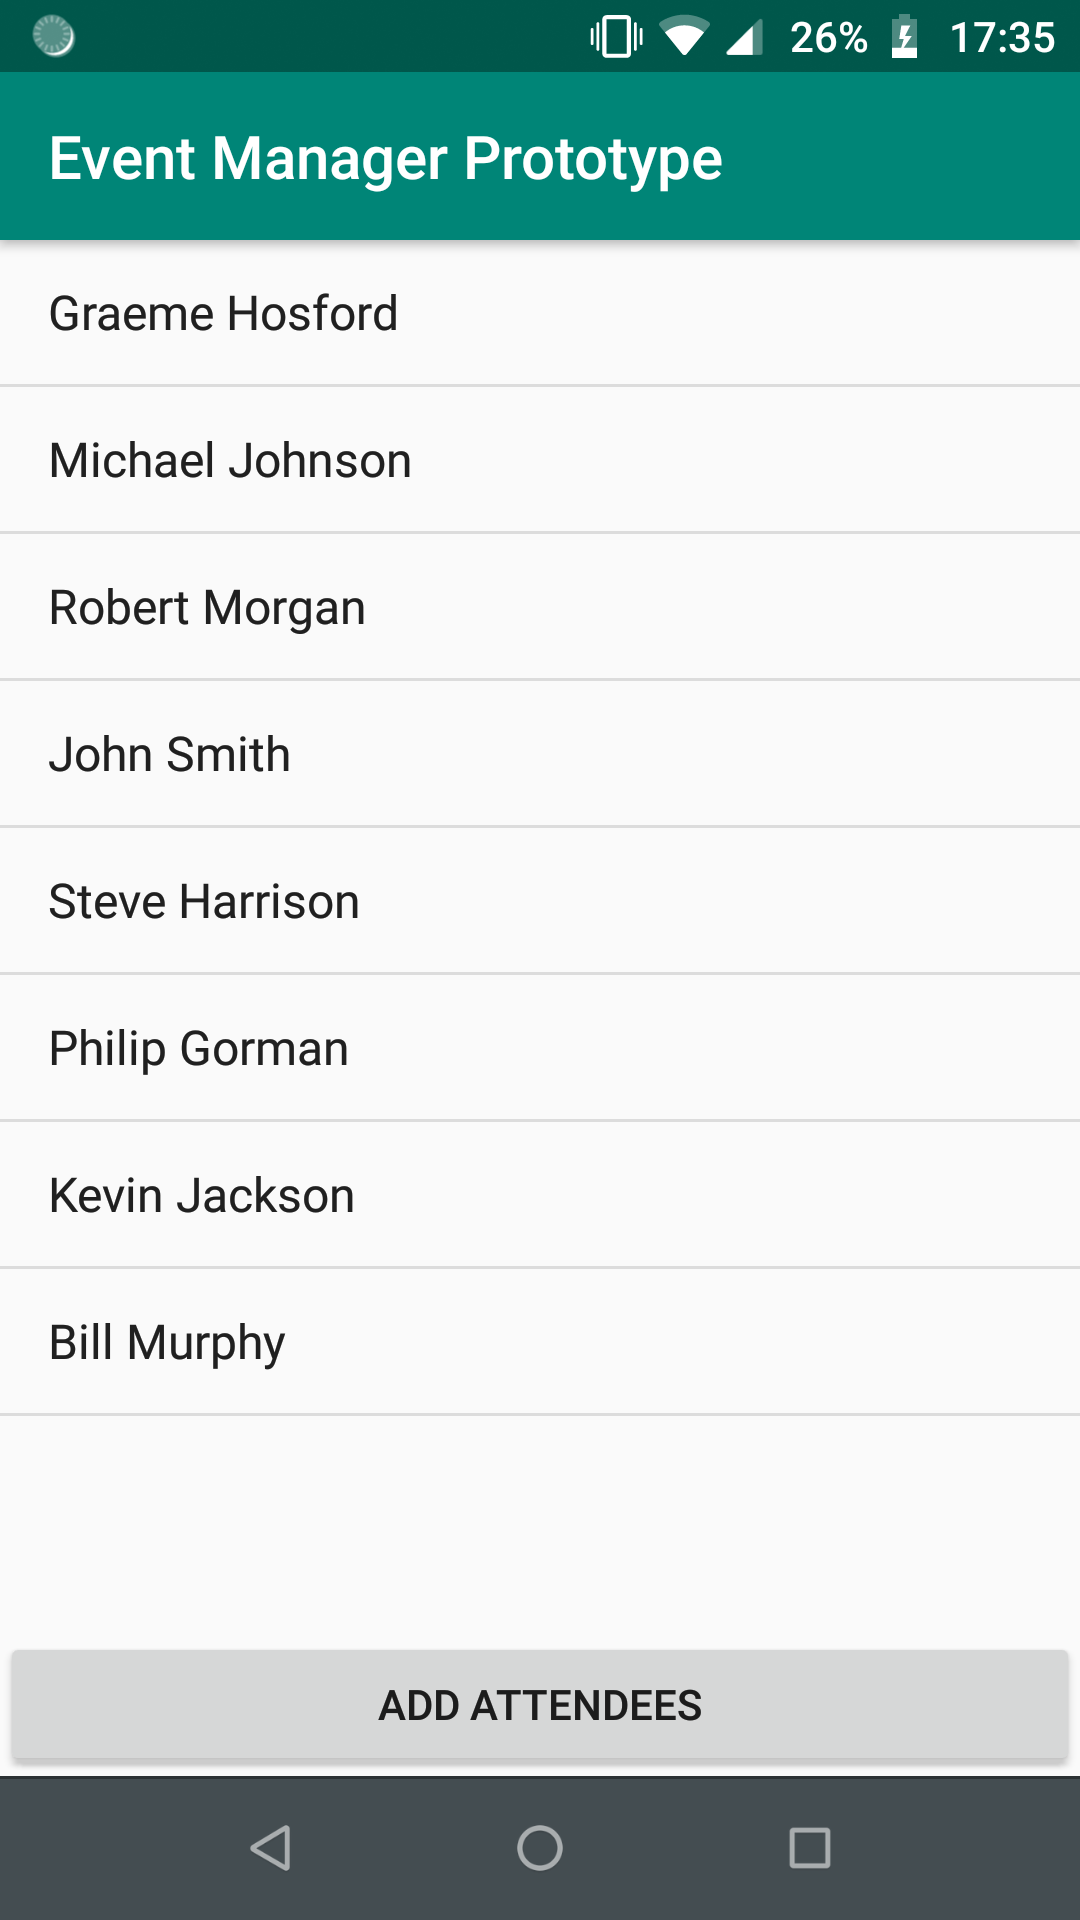
\includegraphics[width=0.7\textwidth]{Attendees.png}
  \caption[Mobile App Prototype Attendees List]{Mobile App Prototype Attendees List}
  \label{fig:AttendeesList}
\end{figure}

The list of attendees for an event can be viewed as shown in Figure \ref{fig:AttendeesList}.

Also provided on this attendees screen is an option to invite more users, this will be an admin-only option and for other users will not be shown.

\clearpage
\begin{figure}[ht]
  \centering
      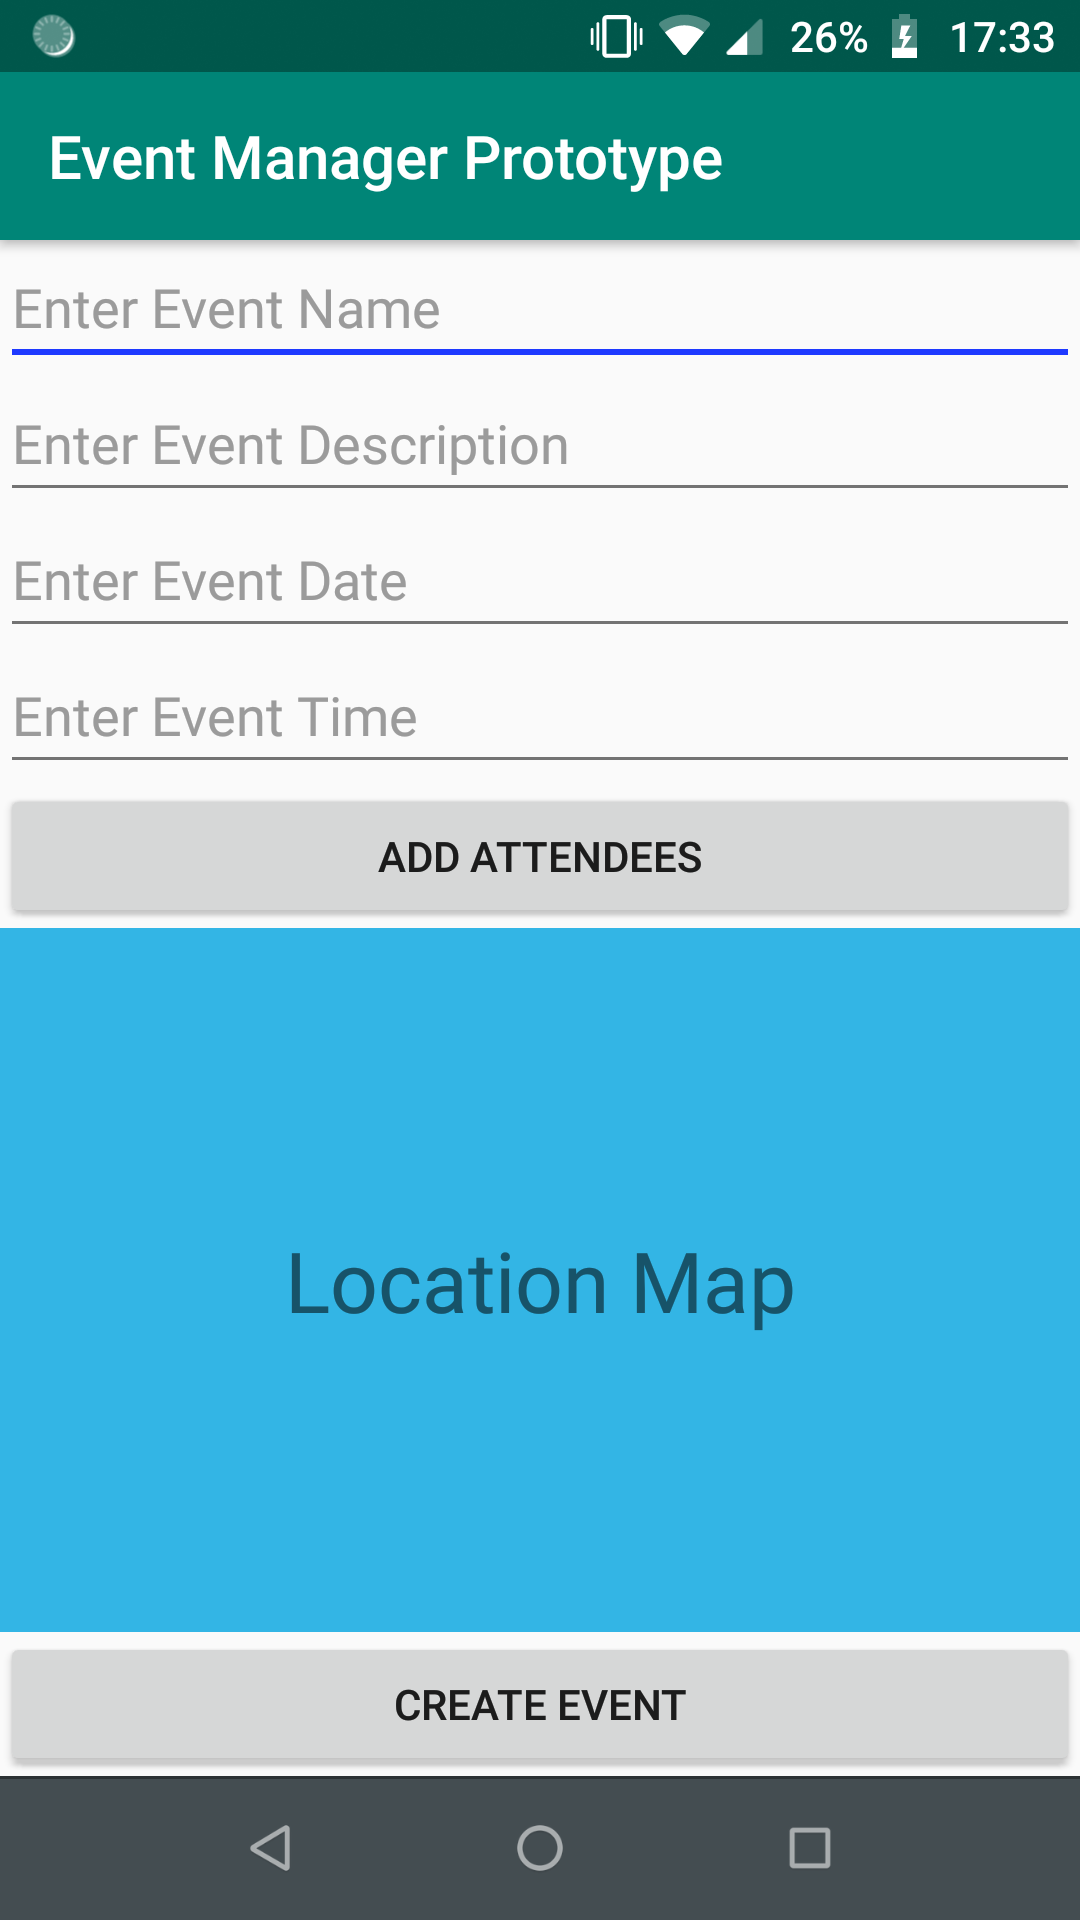
\includegraphics[width=0.7\textwidth]{CreateEvent.png}
  \caption[Mobile App Prototype Create Event Screen]{Mobile App Prototype Create Event Screen}
  \label{fig:CreateEvent}
\end{figure}

When creating an event the screen shown in Figure \ref{fig:CreateEvent} will be presented. This allows the admin to enter the event information which, in turn, will be shown to attendees as in Figure \ref{fig:EventDetail}. The option to add attendees will lead to the same screen as in Figure \ref{fig:AttendeesList}.

\clearpage
\begin{figure}[ht]
  \centering
      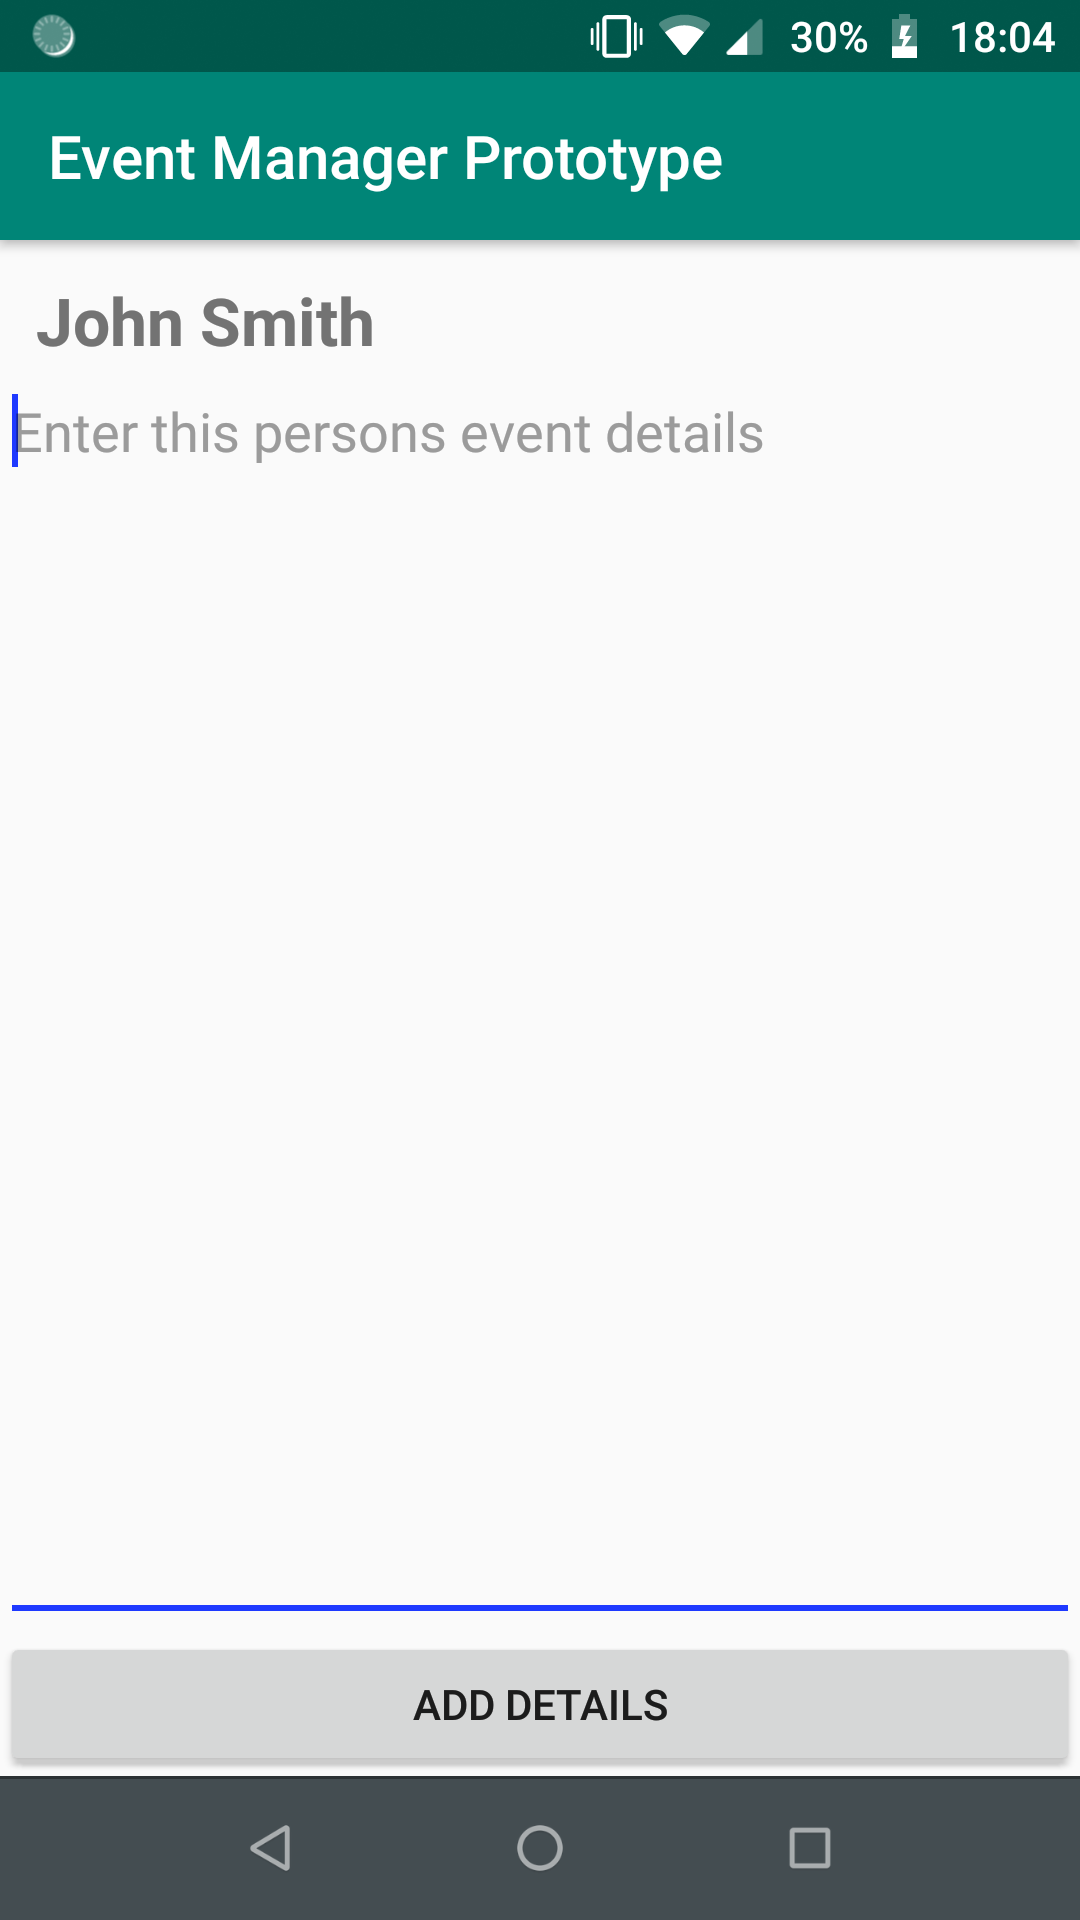
\includegraphics[width=0.7\textwidth]{PersonEventDetails.png}
  \caption[Mobile App Prototype Add Person Event Details Screen]{Mobile App Prototype Add Person Event Details Screen}
  \label{fig:PersonEventDetails}
\end{figure}

When on the attendees list screen as shown in Figure \ref{fig:AttendeesList} an admin may choose to add event specific details to that attendee as shown in Figure \ref{fig:PersonEventDetails}. As there are far too many variable options that an event organiser could add it is deemed easiest to allow a free input through a textbox as shown here rather than trying to create a UI which covers all of the many possibilities.

\clearpage
\begin{figure}[ht]
  \centering
      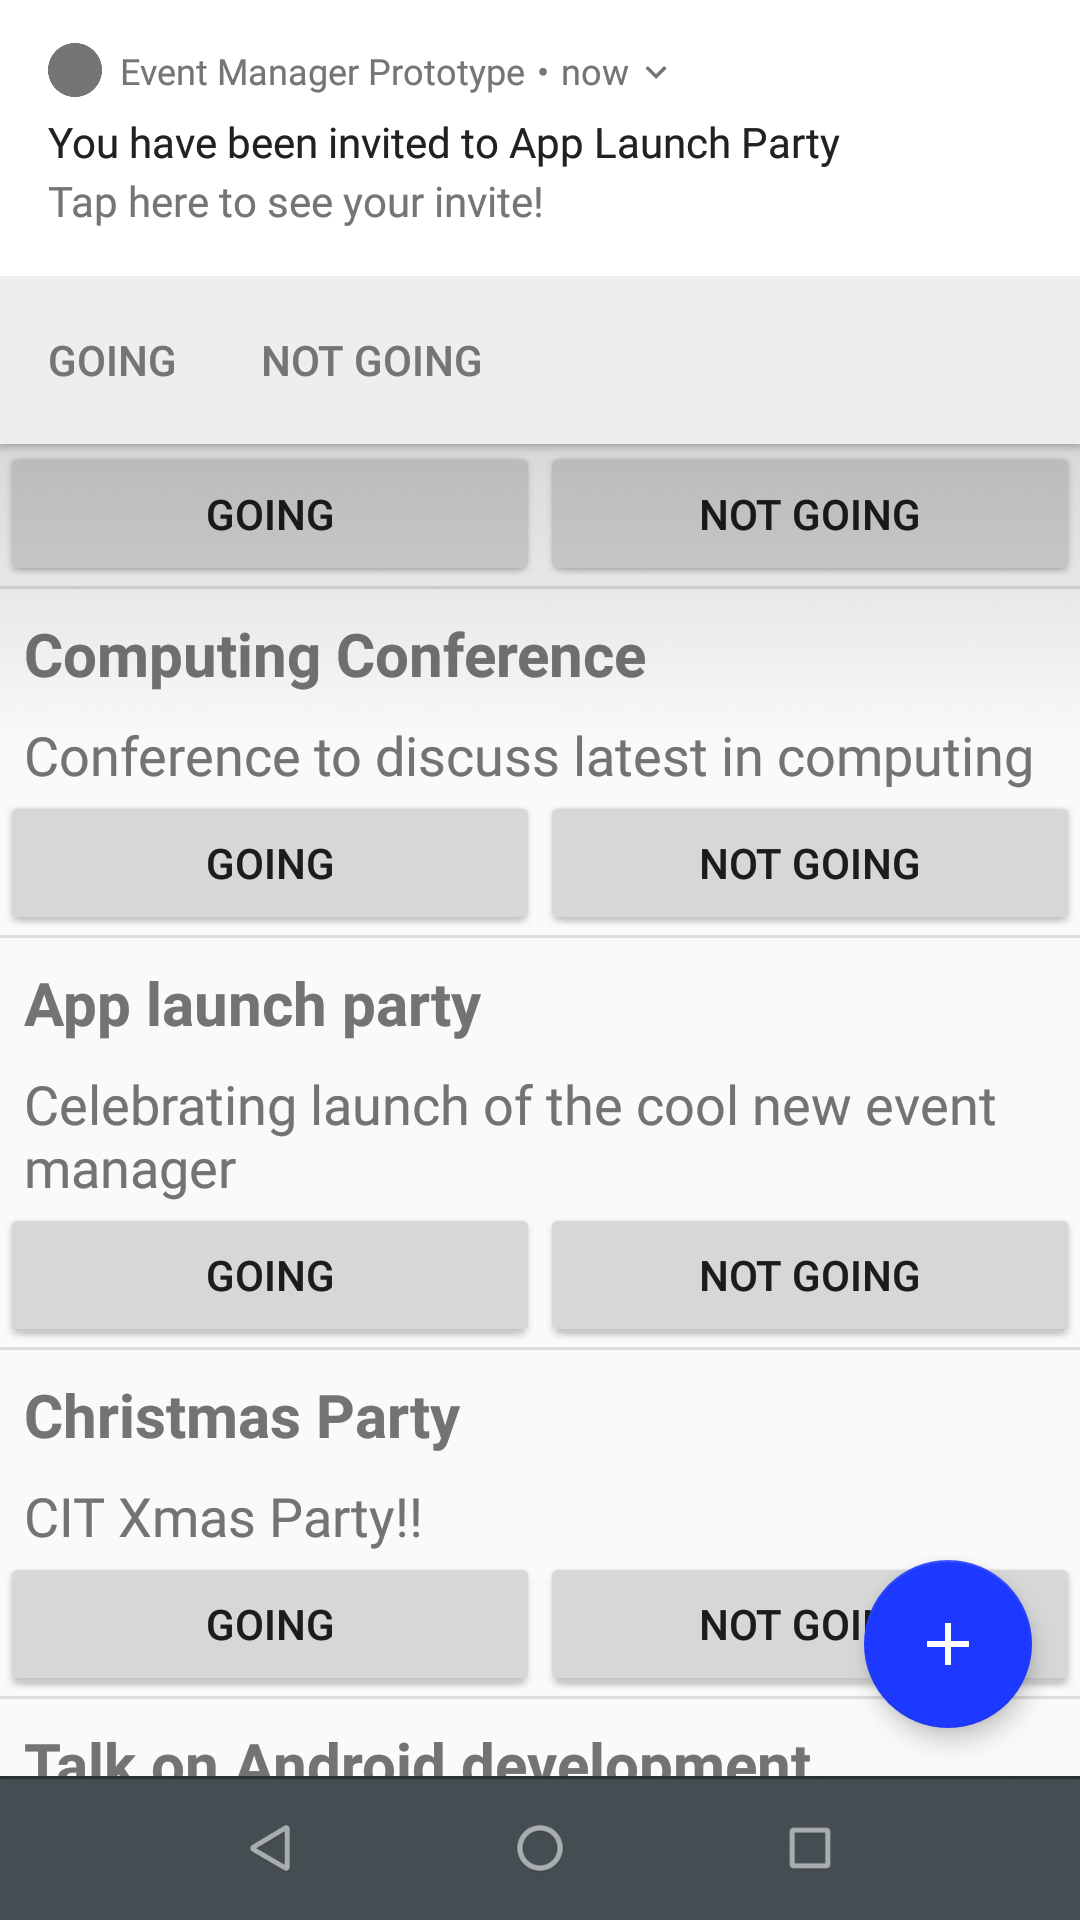
\includegraphics[width=0.7\textwidth]{EventNotification.png}
  \caption[Mobile App Prototype Event Notification Example]{Mobile App Prototype Event Notification Example}
  \label{fig:EventNotification}
\end{figure}

An example of the notifications sent by Firebase when invited to an event is shown in Figure \ref{fig:EventNotification}. A similar notification will be sent when an event thee user has responded to as 'Going' is sent shortly before the event starts as a reminder.

Tapping on the main body of this notification will take the user to view the event details as outlined in Figure \ref{fig:EventDetail}. Also included are shortcut actions to quickly respond to an invite.

\clearpage
\begin{figure}[ht]
  \centering
      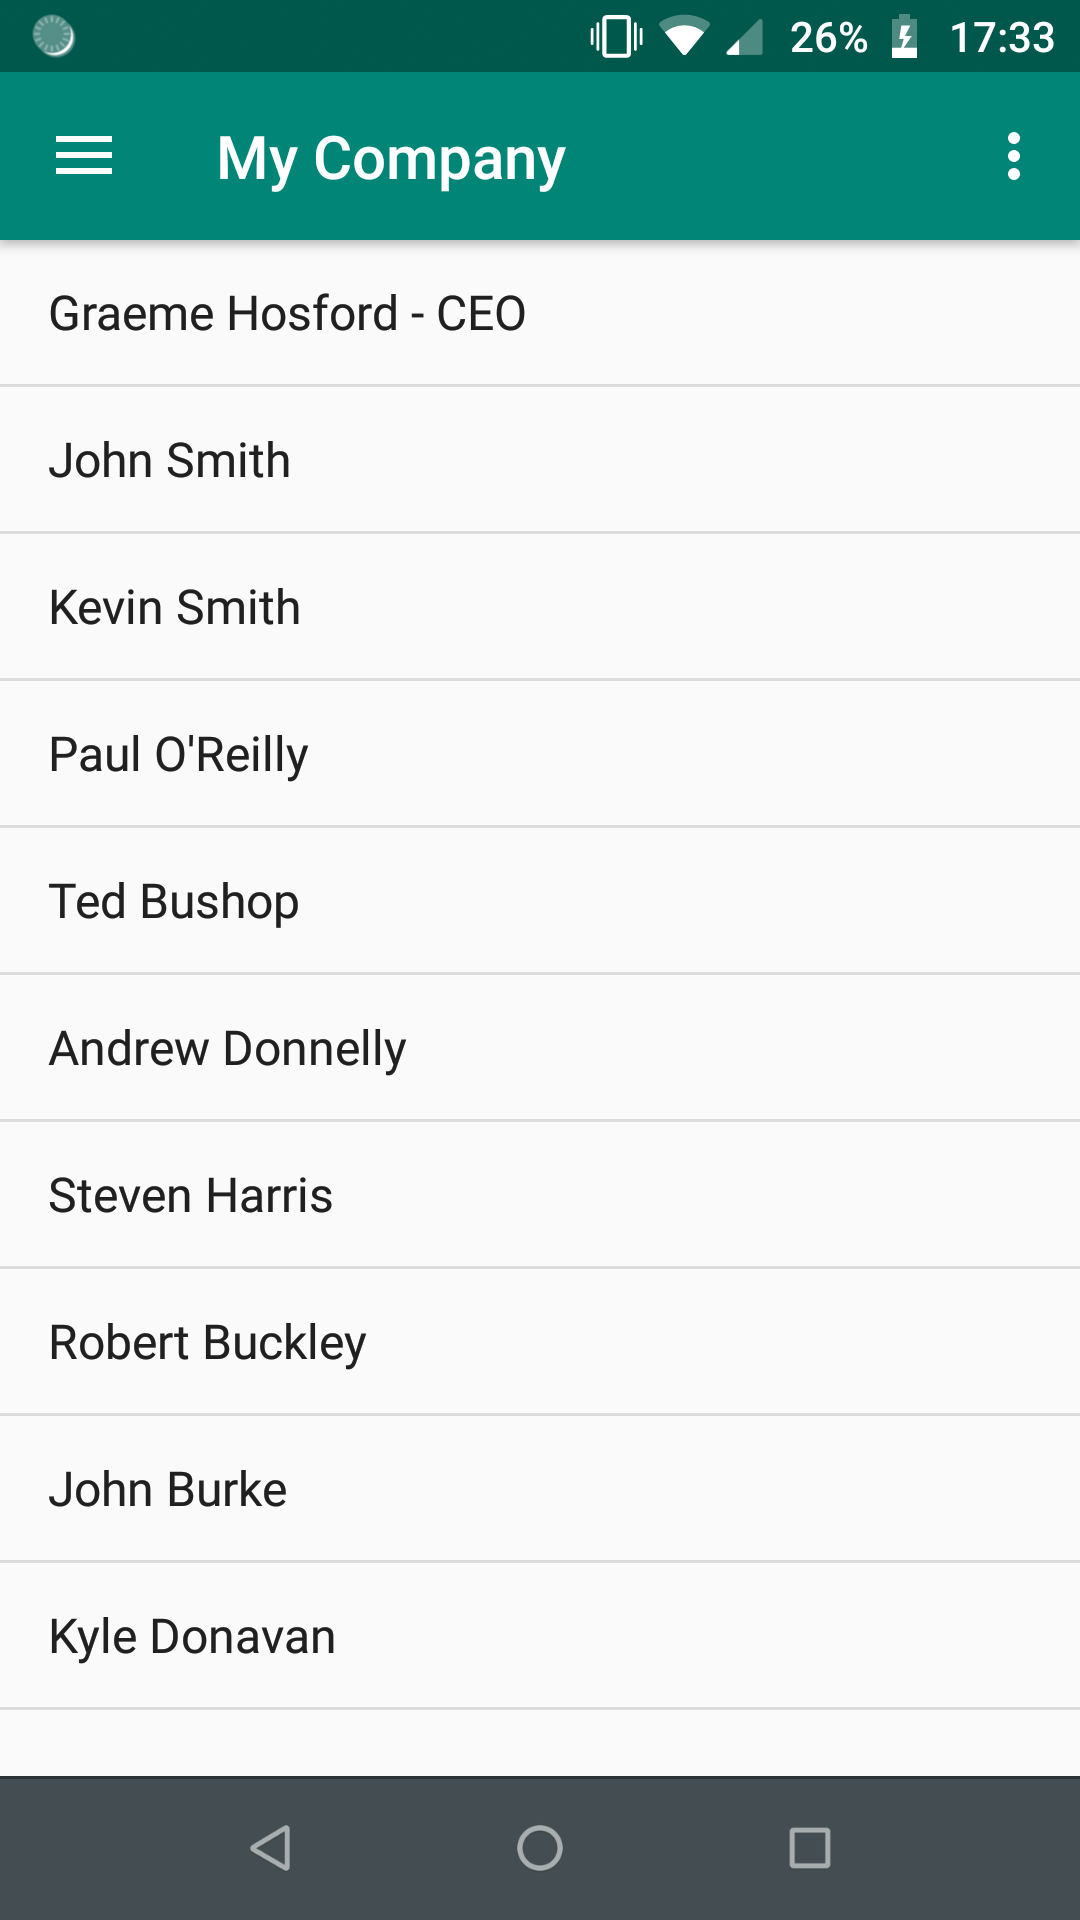
\includegraphics[width=0.7\textwidth]{CompanyMembers.png}
  \caption[Mobile App Prototype Company Details Screen]{Mobile App Prototype Create Company Details Screen}
  \label{fig:CompanyDetails}
\end{figure}

As shown in Figure \ref{fig:CompanyDetails} the user can view the list of members of their own company.

\clearpage
\begin{figure}[ht]
  \centering
      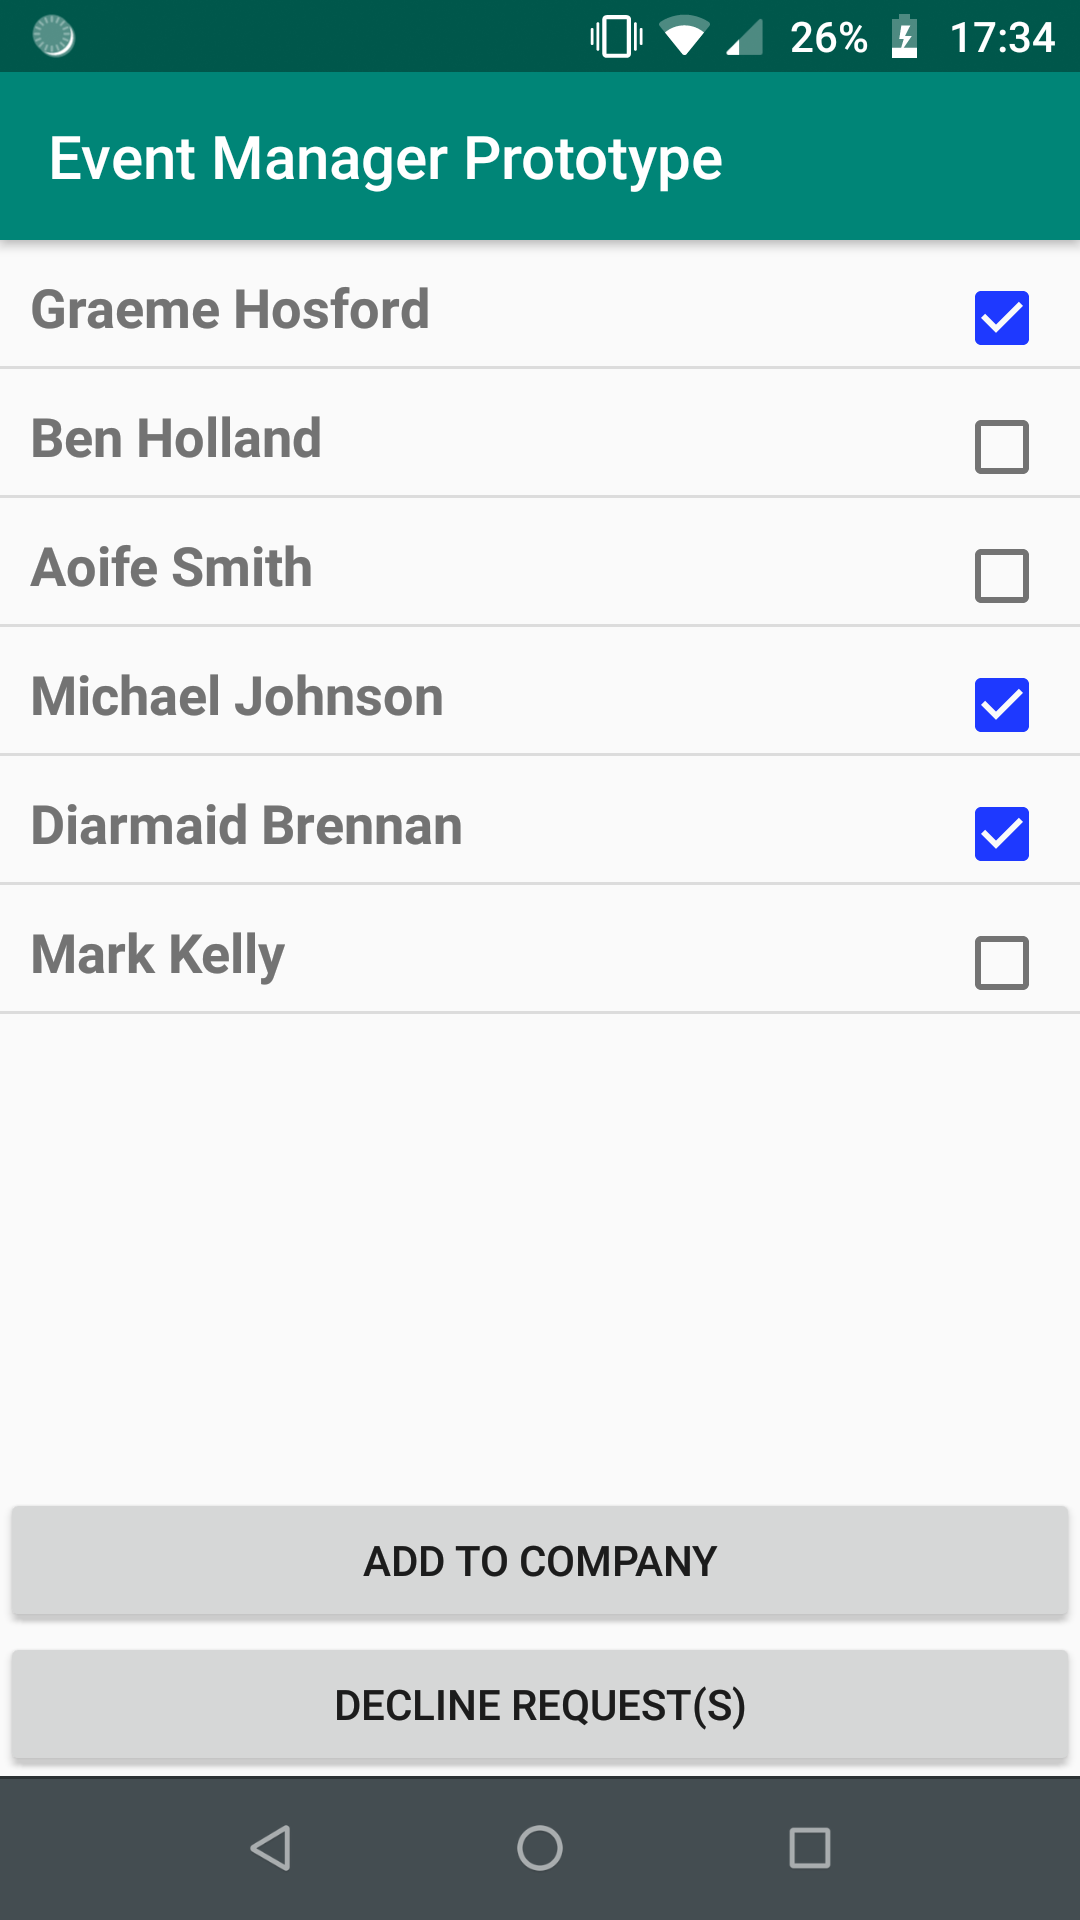
\includegraphics[width=0.7\textwidth]{MemberRequests.png}
  \caption[Mobile App Prototype Company Member Requests Screen]{Mobile App Prototype Company Member Requests Screen}
  \label{fig:MemberRequests}
\end{figure}

In Figure \ref{fig:MemberRequests} is the admin-only feature of approving or denying member requests for the company. Any users added from this list is able to view the company's events and members, and any user whose request is declined simply has their request removed from this list.

\clearpage
\begin{figure}[ht]
  \centering
      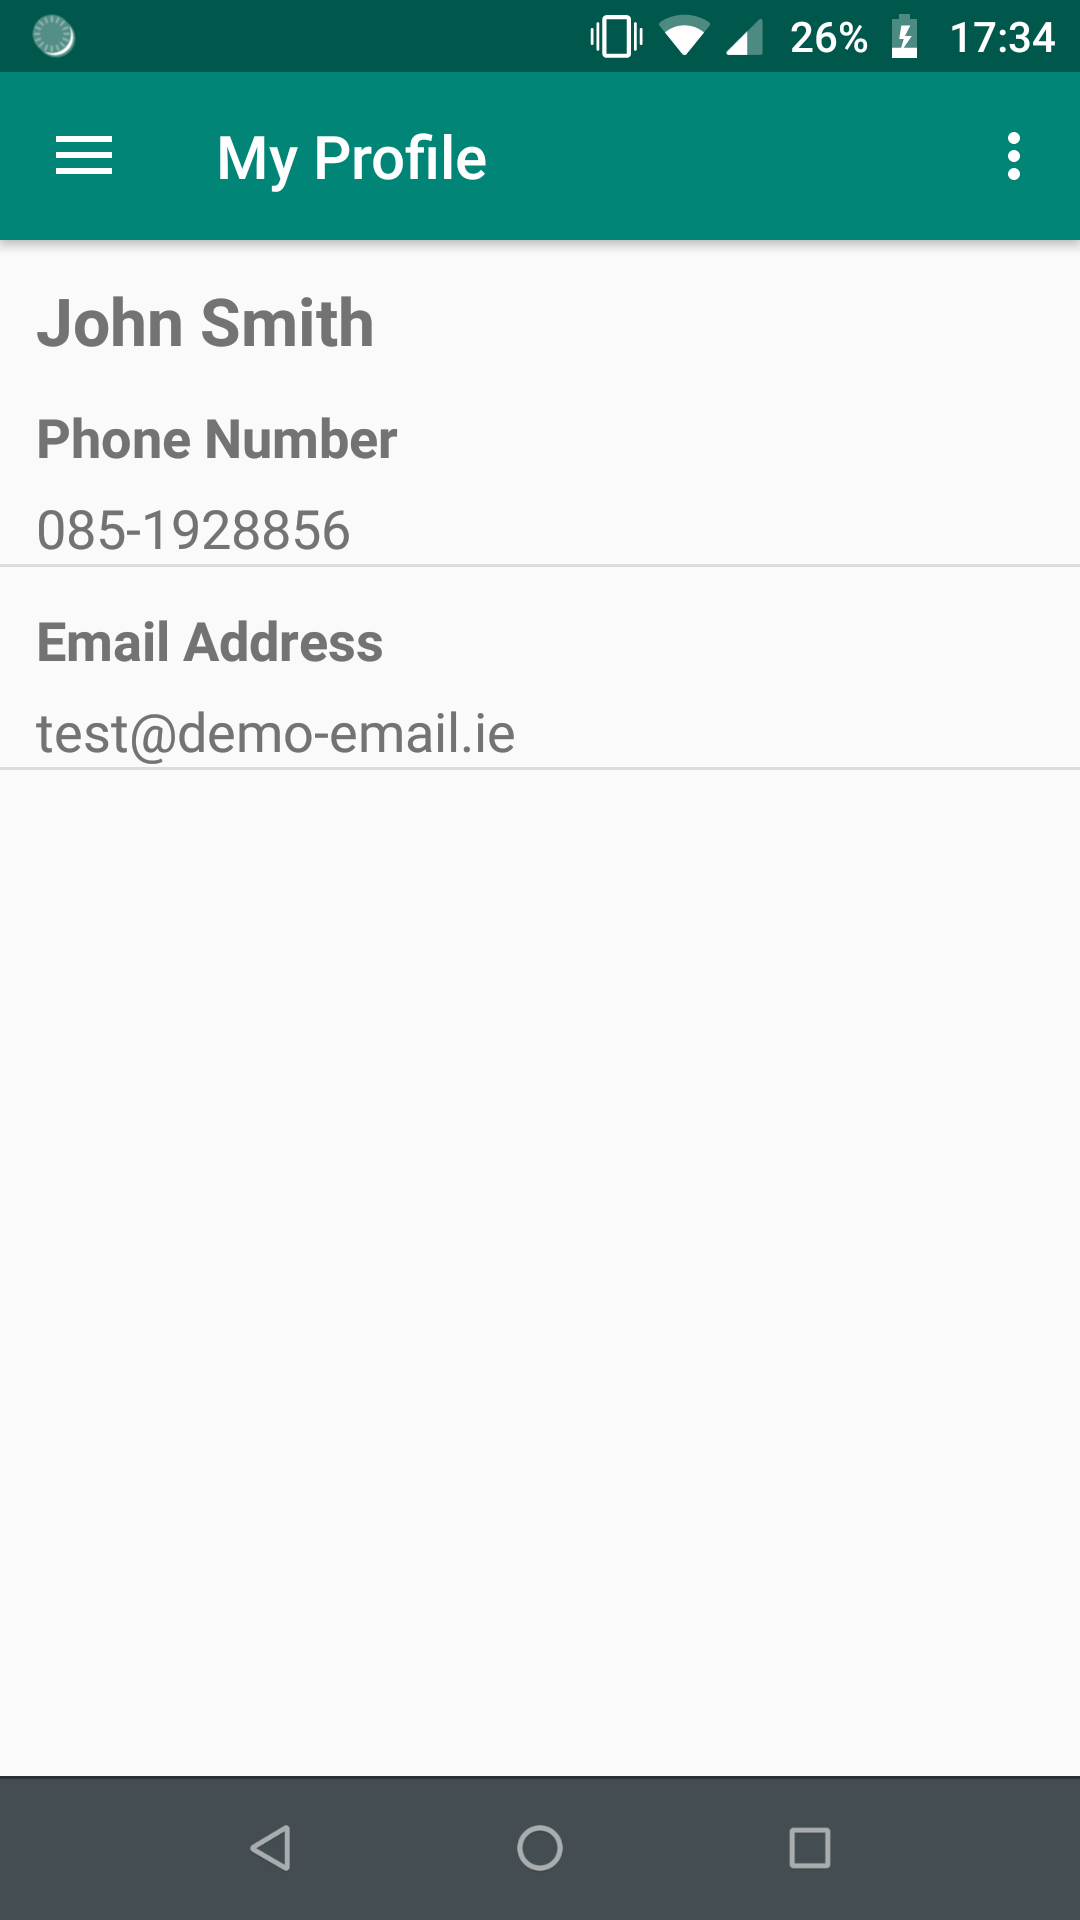
\includegraphics[width=0.7\textwidth]{Profile.png}
  \caption[Mobile App Prototype User Profile Screen]{Mobile App Prototype User Profile Screen}
  \label{fig:UserProfile}
\end{figure}

A user profile is shown in Figure \ref{fig:UserProfile}. A user can view their own profile through choosing the option from the main navigation menu or selecting their own name from the list of company members. The profiles of other users can also be accessed through the member list. 

When a user is on their own profile they also have the option of editing it to change and update the information shown there.

\clearpage % Forcing on to a new page to stop overlap between mobile app and ruby prototypes - Figures are very awkward :/
\subsection{Ruby Server Prototype}

In this section is just the prototype JSON responses for when a new company is created. Unfortunately it was not possible to prototype the notification scheduling here, as again this is mainly Firebase related. Also it was not possible to demonstrate a delayed action. Some prototype output for this however can be seen in Figure \ref{fig:EventNotification}.

\begin{figure}[ht]
  \centering
      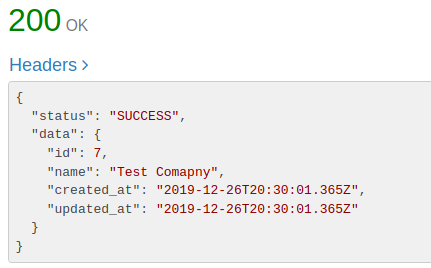
\includegraphics[width=0.7\textwidth]{CompanyPOSTExample.PNG}
  \caption[Ruby Server Prototype Create Company Response]{Ruby Server Prototype Create Company Response}
  \label{fig:CompanyPOST}
\end{figure}

Shown in Figure \ref{fig:CompanyPOST} is the response generated when a new company has been created by the Ruby on Rails server. The key part of this response is the "id" field. As mentioned before the default implementation of Ruby on Rails will automatically generate a simple human readable ID through its database implementation. This ID is then forever associated with the created company and can be entered by users to request to join a company as outlined in Figure \ref{fig:CreateJoinCompany}.

The other fields in this output are considered unnecessary. The company name is included as there must be some piece of data sent to the server to create a database entry and the 'created at' and 'updated at' fields are automatically generated by Rails. All required fields related to the company will instead be saved in Firestore. % Solution Approach

\ifimp
\chapter{Implementation}
\label{chap:imp}
\lhead{\emph{Project Implementation}}
This chapter should comprise 15 pages and enumerate your experience when doing what you wanted to do the way you wanted to do it.

\section{Difficulties Encountered}
Enumerate the different difficulties you have found when developing your solution approach. Create three categories of difficulties:
\begin{itemize}
    \item \textbf{Easy}: You managed to solve the problem with little difficulty.
    \item \textbf{Medium}: It was not easy to solve, but you managed to develop a workaround or solution and still achieve the functionality you originally had in mind.
    \item \textbf{Hard}: The difficulty was so complicated that you didn’t managed to solve it. As a result, some functional requirement / non-functional requirement or use case from your solution approach was not achieved.
\end{itemize}

For each difficulty, classify it into easy, medium or hard. Then, provide the following info:
\begin{enumerate}
    \item Description of the difficulty: Brief description of the problem you found.
    \item How did it affect the original project design?: Indicate how this difficulty affected:
    \begin{enumerate}
        \item the architecture of your solution
        \item if it represented a risk to your project
        \item if it affected your methodology to develop your project
        \item if it changed your implementation schedule
        \item if it changed the evaluation plan
    \item What did you do to manage the difficulty arisen?: Brief description of your decision to overcome the difficulty.
    \end{enumerate}
\end{enumerate}

\section{Actual Solution Approach}
In December of last year, when writing the first version of the report, in Chapter 4 you came up with your original solution approach. On it, you presented (i) the architecture of your solution, (ii) your list of use cases, (iii) a risk assessment, (iv) a methodology to develop your solution approach, (v) your implementation schedule, (vi) your evaluation plan and (vii) some prototype of the resulting product. From January to April you have been developing your solution approach. Along the way you have encountered difficulties (the ones listed in Section 5.1) which might have modified your original plan so that you can come up with an actual developed project.

This section is effectively the production of "as built" specification where you compare your original design to the final finished project. Please go section by section (the ones listed from (i) to (vii) in the last paragraph. For each section, enumerate any difference between the original design and the final project, and justify the difficulty forcing you to make such this change. Do not fret if some of these changes are radical, what is important here is that there is a clear rationale for changes made. % Conclusions and Term 2 work
\chapter{Testing and Evaluation}
\label{chap:eval}
\lhead{\emph{Project Testing}}
The goal of this chapter is an objective evaluation of the final system. The evaluation must be quantitative and not qualitative. You may perform qualitative evaluation but this should not form the basis of the main conclusions you derive from the evaluation. This evaluation, where possible, should be comparative, i.e. you should evaluate your system against a commercially available system and/or system detailed in a research publication. You should demonstrate operational testing of the project using real or contrived data sets to evaluate aspects of the project not encompassed in the software testing (e.g. quantify how well does your project achieved the overall goal). 
\begin{itemize}
    \item For software based projects this will include, but should not be limited to, evaluation of non-functional requirements.
    \item For infrastructural projects this testing should include system/network KPI analysis.
    \item For analysis based projects (ML, malware or other) this may include model evaluation or YARA rule validation, for example.
    \item For management projects, where software testing or infrastructure testing may not be in scope, the test process for the system is expected to be more rigorous and well described than a project incorporating significant development work.
\end{itemize} 

Some suggested sections (the nature of this chapter should be discussed in detail with your term 2 supervisor):

\section{Metrics}
Identify and describe the metrics you used to evaluate your project. You should have identified some of these in the research phase report but will detail these as you progress through the design.

\section{System Testing}
Describe the experimental setup for each metric, and how you obtained the measurements. Describe the inputs for each experiment

\section{Results}
Summarise the output data, and the statistical or other techniques to deduce your results. Summarise your results, including tables or graphs as appropriate with a brief description of each. here possible, compare your results with other products/systems. Identify any possible threats to the validity of your results, and discuss each briefly here (you will discuss in more detail in the next chapter). % Conclusions and Term 2 work
\chapter{Discussion and Conclusions}
\label{chap:conclusions}
\lhead{\emph{Discussion and Conclusions}}
In this chapter, you should expand upon (and initially reflect upon) the discussion and conclusion of the research phase of the project. The expectation here is that you should discuss the results presented in the previous evaluation section of the project in their totality (i.e. as a whole) from which you will then draw clear conclusions both on the quantitative and qualitative aspects of the overall project. This chapter should be a about 2000 words long (5 pages of text - 1600 words of discussion and 400 words of conclusion). This may vary depending on quality. The conclusion section of this report should conclude the project.

Some suggested sections (the nature of this chapter should be discussed in detail with your term 2 supervisor):

\section{Solution Review}
Discuss how well your solution solves the problem, based on your results from the evaluation chapter.

\section{Project Review}
Discuss how well you addressed the project, and what you might do differently if you were to do it again. Make sure to identify how you handled any problems that arose during the project. Identify key skills that you learnt during the project, and clearly describe how you applied these, and how you might apply them differently if you were to do a similar project.

\section{Conclusion}
Enumerate the main conclusions you have got in terms of background, problem description and the solution approach you have come up with. Detail your primary and any secondary conclusions from your project.

\section{Future Work}
Discuss any proposals for completion of the project, or for enhancements, or for re-design of your solution or software. Enumerate all the things you would have wanted to do should you have more time to work on this project. % Conclusions and Term 2 work
\else
\chapter{Conclusions and Future Work}
\label{chap:conclusions}
\lhead{\emph{Conclusions}}
% This chapter should comprise 2-3 pages and enumerate conclusions of this phase of work. In your final report Discussions and Conclusions will form separate chapters and be significantly longer and more detailed.

\section{Discussion}
\label{section:discussion}
% A reflective discussion of some of the problems you encountered during this phase of the project and how that may influence how you proceed with the next phase.

In reflecting on difficulties encountered in this research phase I find that the only major issue I had was translating research down onto paper. However I believe this problem occurred due to attempting to write this report while doing research concurrently. I changed this approach relatively early during the semester and found progress was much smoother afterwards. 

In regards to implementation work I think the best way to translate this improvement in work process is to put report writing on the sidelines until I have entire parts of the implementation completed, rather than attempting to write parts of the report while the associated part of the implementation is only partway completed.

A very minor issue encountered during this phase was time management. While I was generally able to find ample time enough to invest into this report, unavoidable time constraints caused by assignments in other college modules often lead to not being able to invest the desired time into this report.

For the implementation phase I believe this will be less of an issue to begin with as I will be doing my best to strictly adhere to the sprint schedule outlined in section \ref{section:implementationplan}. Considering I have a sizable amount of experience working with Android for about 6 years now, both as a hobby and a job, I think it is likely I can finish most sprints a day or two early and invest that remaining time into report writing and completing other college work. This should in turn free up the schedule of future sprints a bit more to allow for more project focus.

Besides these, the only other problem faced was trying to find relevant sources for research. However this will not be a reoccurring point during implementation as research is completed.

\section{Conclusion}
\label{section:conclusion}
% Enumerate the main conclusions you have got in terms of background, problem description and the solution approach you have come up with.

With the research phase of this project now complete, there is now a good overview of the problem being tackled along with the proposed solution.

As stated at the beginning of this report the initial problem statement came to me during my time working in Teamwork where the HR department had several issues related to event organisation with large numbers of attendees.

While this project does not aim to tackle only these specific issues, the initial idea grew into the project as it is today which takes a slightly broader approach in addressing the problem. in effect meaning this is a more generic solution rather than a Teamwork specific solution.

Given the problems often associated with event management on a large scale, the proposed system will help to tackle many organisation related issues as this is where the majority of problems stem from.

\section{Future Work}
\label{section:futurework}
% Enumerate all the things you would have wanted to do should you have more time to work on this report.

In regard to further developing this report I briefly considered including a desktop application and its associated research in this project. However, I eventually decided that such an extra, major piece added to this proposed system would be unlikely to be completed and only further strain already limited time. I believe this would have been a great addition to this project but in hindsight I believe I made the right choice in leaving it out as I wouldn't have had the time to research it, and likely would not have the time either to develop it in the project implementation phase. 

I also wanted this to be a mobile-first project, as this is the way in which users are most increasingly accessing online services, and therefore a mobile-first approach lends to allowing greater access to the app being developed. Given this point I further felt that attempting to add in a desktop application would take time away from making the mobile app as well made as possible.

Aside from the desktop application I also very briefly considered a web-based application but I am very inexperienced in web development, having only a passing knowledge of some server side development. Any attempt to develop a frontend web app would most likely end with a poorly made product and again, time taken away from the mobile app thus lessening what can be accomplished there.

% Additional resources on the use of latex is below.

% Tutorials:
% \begin{itemize}
%     \item \url{https://www.latex-tutorial.com/tutorials/beginners/how-to-use-latex}
%     \item \url{https://en.wikibooks.org/wiki/LaTeX}
%     \item \url{https://www.sharelatex.com/learn/Main_Page}
%     \item \url{http://www.math.harvard.edu/texman}
%     \item \url{https://web.stevens.edu/hfslwiki/images/a/a0/ShareLatex_Tutorial.pdf}
% \end{itemize}

% Presentations:
% \begin{itemize}
%     \item \url{http://www.iu.hio.no/~frodes/rm/ppt/latex.ppt}
%     \item \url{https://classes.soe.ucsc.edu/ams200/Fall09/Latex_intro.ppt}
%     \item \url{http://www.menet.umn.edu/~blake/latexcourse/courseslides.ppt}
% \end{itemize}
 % Conclusions and Term 2 work
\fi
%% ----------------------------------------------------------------
\label{Bibliography}
\bibliographystyle{IEEEtranN}  % Use the "IEEE Transaction" BibTeX style for formatting the Bibliography
\bibliography{Bibliography}  % The references (bibliography) information are stored in the file named "Bibliography.bib"
\lhead{\emph{Bibliography}}  % Change the left side page header to "Bibliography"

%% ----------------------------------------------------------------
% Now begin the Appendices, including them as separate files

\addtocontents{toc}{\vspace{2em}} % Add a gap in the Contents, for aesthetics

\appendix % Cue to tell LaTeX that the following 'chapters' are Appendices

\chapter{Code Snippets}

Put appendix material in this section e.g. code snippets 

USE THE APPENDICES	% Appendix Title

\chapter{Wireframe Models} % Appendix Title

%\input{Appendices/AppendixC} % Appendix Title

\addtocontents{toc}{\vspace{2em}}  % Add a gap in the Contents, for aesthetics
\backmatter
\end{document}  % The End
%% ----------------------------------------------------------------